\documentclass[referee, pdflatex, sn-mathphys-num]{sn-jnl}

\usepackage{hyperref}
\usepackage{geometry} 
\usepackage{subfigure}
\usepackage{graphicx} 
\usepackage{amsmath,amsfonts,amssymb,amsthm,mathtools}
\usepackage{icomma}
\usepackage[english]{babel}
\usepackage{array,tabularx,tabulary,booktabs}
\usepackage{multirow}
\usepackage{diagbox}

\theoremstyle{definition}
\newtheorem{Def}{Definition}
\theoremstyle{plain}
\newtheorem{Lem}{Lemma}
\newtheorem{Th}{Theorem}
\newtheorem{Prop}{Property}

% article-specific symbols
\newcommand{\delayV}[1]{\overset{\leftarrow}{\mathbf{x}}_{#1}}
\newcommand{\delayM}[1]{\overset{\leftarrow}{X}_{#1}}

\begin{document}
	
	\title{Tensor decomposition and forecasting for multivariate time series}
	
	\author*[1]{\fnm{Kirill} \sur{Semkin}}\email{kirill.semkin32@mail.ru}
	\author*[2]{\fnm{Vadim} \sur{Strijov}}\email{strijov@ccas.ru}
	
	\affil*[1]{\orgname{Forecsys$^\text{{\footnotesize \textregistered}}$} \orgaddress{\city{Moscow}} \country{Russia}}
	\affil*[2]{\orgname{Forecsys$^\text{{\footnotesize \textregistered}}$} \orgaddress{\city{Moscow}} \country{Russia}}
	
	\keywords{time series, decomposition, forecast, SSA, CPD}
	
	\maketitle
	
	\begin{abstract}
		
		Processing of multidimensional time series is associated with an additional task of determining dependencies between signals. Its inclusion in models boosts the quality of forecasts. On the other hand, taking this dependency into account makes models more complex and less interpretable. The paper proposes a non-parametric method based on tensor data representation and Singular Spectrum Analysis (SSA). It derives a time series decomposition technique and an explicit forecast model. Finally, it applies an elaborated theory to electricity consumption and inertial measurement unit datasets. It compares the obtained quality of forecast with mSSA, VAR, and RNN models.
		
	\end{abstract}
	
	% TODO: series -> time series
	% TODO: Fig. 1, обозначение из рисунка вставить в текст
	% TODO: Приклеить формулы к тексту
	% TODO: 
	% TODO: 
	% TODO: 
	
	\section{Introduction}\label{Intro}
	
	The main object of the paper is multivariate time series. It is a set of $ m $ series $ \{x_i(t)\}_{i=1}^m $ observed in discrete time $ t \in 1 , \ldots , N $.	We state two problems concerning them. First, to make a \emph{forecast} is to estimate future values $ \{x_i(T)\}_{i=1}^m $ of the series at time $ T > N $. Second, to build an additive \emph{decomposition} is to represent each signal in a set as a sum of several components: $ x_i(t) = c_1(t) + \ldots + c_s(t), \ \forall i \in 1, \ldots , m $.
	
	For the decomposition in a single-variate time series case, the papers~\cite{enders2010applied, x11, cleveland90} introduce seasonal-trend-cycle techniques. For the forecast, the authors in~\cite{Box_Jenkins_methodology} propose autoregressive methods as well as works~\cite{3b1355aedd1041f1853e609a410576f3, enders2010applied} suggest exponential smoothing, regression models, and neural networks. However, these methods can not be transferred to the multivariate series straightforwardly if they are interdependent. The paper~\cite{Volterra:1928} models the size of prey-and-predator populations as a coupled system of differential equations. The dynamics of one population depends directly on the other's and vice-versa. Therefore the forecast can not be made separately. 
	
	Some methods both take into account multivariate time series interdependence and make the forecast. First, \emph{recurrent neural network} (RNN)~\cite{neco} connects series and their past values through several layers of nonlinear transformations. Information from the past values is encapsulated in the hidden state vector at each time step. It is used to forecast future values~\cite{TEALAB2018334}.
	
	Second, the	\emph{vector autoregression} (VAR)~\cite{VAR_model1, doi:10.1080/01621459.1962.10480664} is a linear stochastic model for multivariate series. Denote vector $ \mathbf{x}_t = (x_1(t) \ldots x_m(t))^{\mathsf{T}} $ as a series realizations at time $ t $, their further dynamics
	
	\begin{equation*}
		\mathbf{x}_t = \boldsymbol{\mu} + \sum\limits_{i = 1}^p A_i \mathbf{x}_{t - i} + \mathbf{u}_t.
	\end{equation*}

	
	Here  $ \boldsymbol{\mu} $ is a constant vector, $ A_i $ are $ m \times m $ matrices, $ \mathbf{u}_t $ is a random vector (e.g. white noise $ \text{WN}(t) $). The time series interdependence is defined by $ A_i $ matrices, so each series depends on each other and their past linearly.
	
	The RNN and VAR methods are able to make the forecast, but, firstly, have a large number of learnable and structural parameters. That means their underlying models have an extensive complexity. Their architecture needs to be picked over and tuned. Secondly, the methods' structure does not contain an explicit way of building series decomposition.
	
	To rectify the listed disadvantages, we have developed a new method called the \emph{tensor SSA} (tSSA). It has only two adjustable parameters. The tSSA extends the SSA method~\cite{ecfb9dc578be43ae9ee8fc88b8ff9151} for the multivariate time series and implies using dynamical systems theory. The Takens theorem~\cite{citeulike:2735031} is the theoretical foundation of the tSSA. \emph{Hankel} matrices and their properties are involved in the decomposition problem. It is a matrix with equal elements on each anti-diagonal. Such matrices are tightly connected with Toeplitz and circulant matrices.
	
	The main task of the paper is to find the shared \emph{phase subspace}~\cite{1572261550523548160, ignatov2016human} for all observed time series. This is a low-dimensional linear subspace where all the system's trajectories can be mapped into isomorphically. Finding it enables us to obtain phase representation of the observed series. Fig.~\ref{pic:phase_traj} illustrates this idea. We use a single time series to build phase space and the specific trajectory of the dynamical system that generated the given series. The forecast then is found upon the fact that the continuation of the trajectory lies in the very same phase space. Partitioning basis vectors of this space into several groups builds the decomposition of the series. The paper develops named conceptions in the next sections.
	
	\begin{figure}[!htbp]
		\centering
		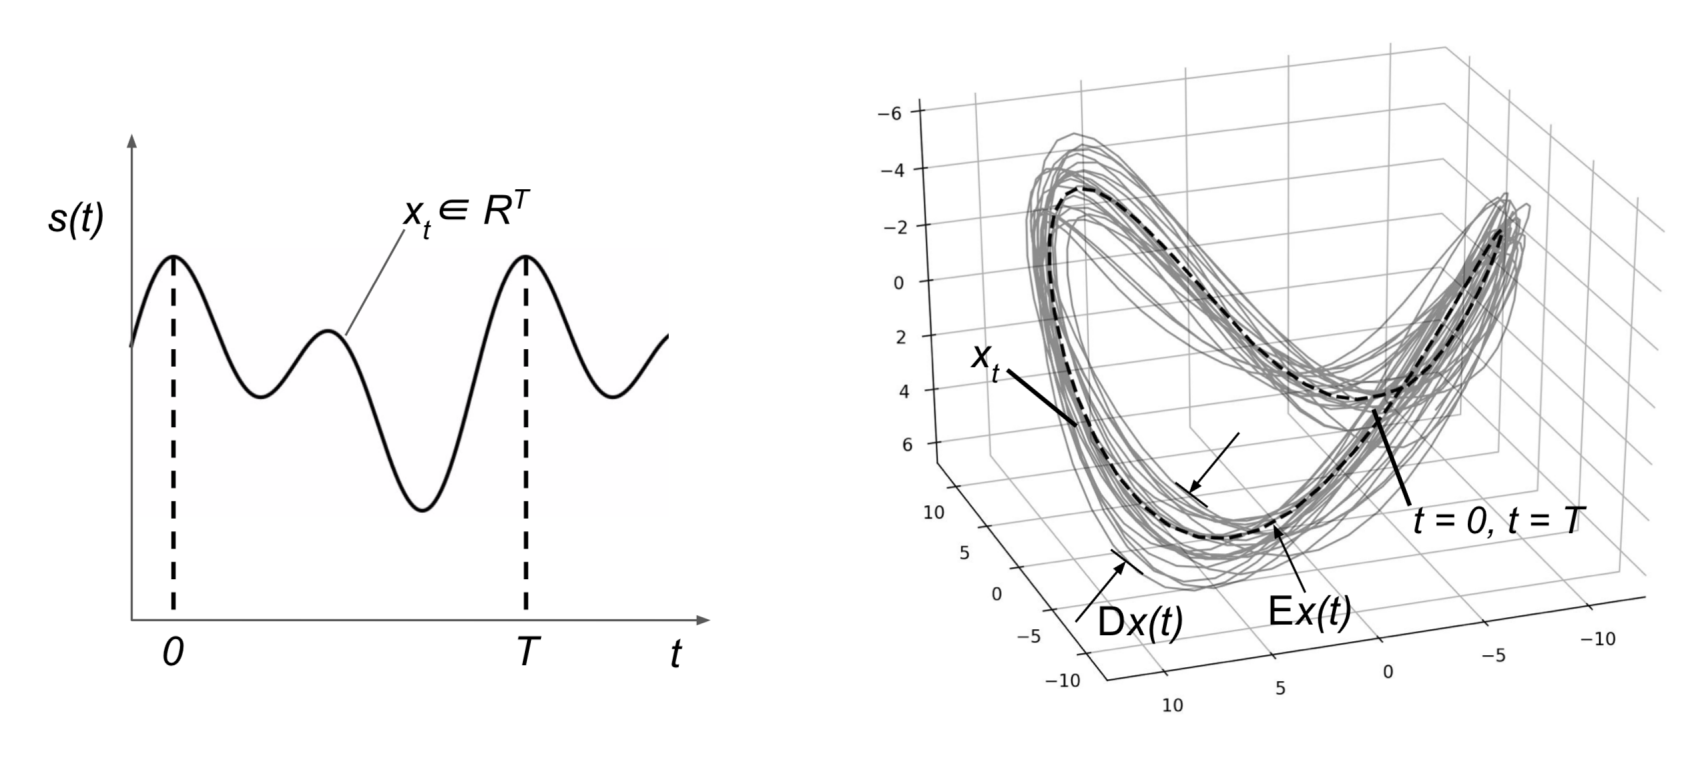
\includegraphics[width=0.9\textwidth, keepaspectratio]{phase_traj.png}
		\caption{Time series's phase trajectory visualization }\label{pic:phase_traj}
	\end{figure}
	
	Our method captures autocorrelation and multilinearity of the time series via tensor data representation. \emph{Canonical polyadic decomposition} (CPD) is used to build the phase space of the series. Another solution is to use matrix data representation and matrix decompositions. Such method is called matrix SSA (mSSA)~\cite{mSSA_overview}. It is the second extension of the SSA method for the forecast and the decomposition of the multivariate time series. The tSSA is compared with the mSSA in the computational experiment section.
	
	The rest of the paper covers the theory and application of our method to real data. Firstly, the dynamical systems model is introduced and the problem of basis search in the phase space is stated and resolved. These results enable us to propose a way of decomposing the series and to make the forecast. Simultaneously, features of obtained solutions are examined and two associated theorems are formulated. Finally, tSSA and mentioned methods are applied to two datasets: electricity consumption and accelerometer/gyroscope observations. We obtain their forecast and additive decompositions. For the latter, a special quality metric is introduced.
	
	\section{Problem statement}\label{sec:problem_statement}
	
	Suppose a \emph{dynamical system} defined on $ X $, with the evolution function $ f $ and the initial state $ \mathbf{y}_0 $. Time space is discrete
	
	\begin{gather*}
		\mathbf{y}(t + 1) = f \bigl( \mathbf{y}(t) \bigr), \quad \ t \in \mathbb{N}, \\
		\mathbf{y}(0) = \mathbf{y}_0 .
	\end{gather*}
	
	Generally, $ X $ is a high-dimensional smooth manifold. Then unknown mapping $ \boldsymbol{\phi}: X \to \mathbb{R}^m $ takes each trajectory point $ \mathbf{y}(t) $ to the multivariate time series realization $ \mathbf{x}_t $
	
	\begin{equation*}
		\boldsymbol{\phi} \bigl( \mathbf{y}(t) \bigr) = \mathbf{x}_t. \text{ Coordinately:} \begin{cases}
			\phi_1 \bigl( \mathbf{y}(t) \bigr) = x_1(t), \\
			\ldots \\
			\phi_m \bigl( \mathbf{y}(t) \bigr) = x_m(t). \\
		\end{cases}
	\end{equation*}
	
	Assume that the trajectories $ \mathbf{y}(t) $ belong to the smaller dimension manifold $ M \subset X $. Now the problem is to find an embedding of the $ M $ into $ \mathbb{R}^{L} $ for some $ L $. The second problem is to build a basis in the image of the embedding. Having done that, the initial dynamical system will be described in terms of the standard linear space. The same will hold to all time series $ x_i(t) $.

	\section{Single-variate series case}\label{sec:one_series}
	
	The tSSA relies on the SSA method and the Takens theorem. The theorem provides the needed embedding in the single-variate series case. Any point $ \mathbf{y}(t) \in M $ corresponds to the following vector:
	
	\begin{equation*}
		\bigl( \, \boldsymbol{\phi} \circ f^{t - L + 1} \bigl( \mathbf{y}(t) \bigr), \ldots , \boldsymbol{\phi} \circ f \bigl( \mathbf{y}(t) \bigr), \boldsymbol{\phi} \circ \mathbf{y}(t) \, \bigr)^{\mathsf{T}} = \bigl( x(t - L + 1), \ldots , x(t-1), x(t) \bigr)^{\mathsf{T}}.
	\end{equation*}
	
	
	It is called the \emph{delay vector} at time $ t $ and is denoted as $ \delayV{t} $. The vector's dimension $ L $ must satisfy condition $ L > 2 \cdot \dim(M) $. The function $ \phi(\cdot) $ must satisfy several regularity conditions. They are omitted here and considered fulfilled.
	
	Now the time series $ x(t) $ with the length $ N $ gives $ N - L + 1 $ delay vectors. Therefore image of the embedding is $ \text{Lin}(\{\delayV{t}\}) $. It represents the \emph{individual} phase space of the series and must be low dimensional. This means $ \text{Lin}(\{\delayV{t}\}) \subset \mathbb{R}^L $. Finally, the orthonormal basis is an $ U $-component of the Singular value decomposition (SVD) on the \emph{trajectory matrix} $ H_x $. It is a stacking of the delay vectors
	
	\[
		H_x = [ \delayV{1} \ldots  \delayV{N - L + 1}].
	\]
	
	\section{Multivariate series case and the tSSA method}\label{sec:tssa_method}
	
	Now there given multivariate time series. Let $ m $ be their number. Hence, the $ \boldsymbol{\phi}(\cdot) $ is a multidimensional map. This means that instead of the single delay vector we have $ m $ of them at any time $ t $. Let $ \delayM{t} $ be a matrix $ [ \delayV{1_t} \ldots \delayV{m_t} ] $ called the \emph{delay matrix}. Then, the embedding image is a linear span of all $ \delayM{t} $. It is also called the \emph{shared} phase space of the multivariate time series.
	
	\begin{figure}[!htbp]
		\centering
		\subfigure{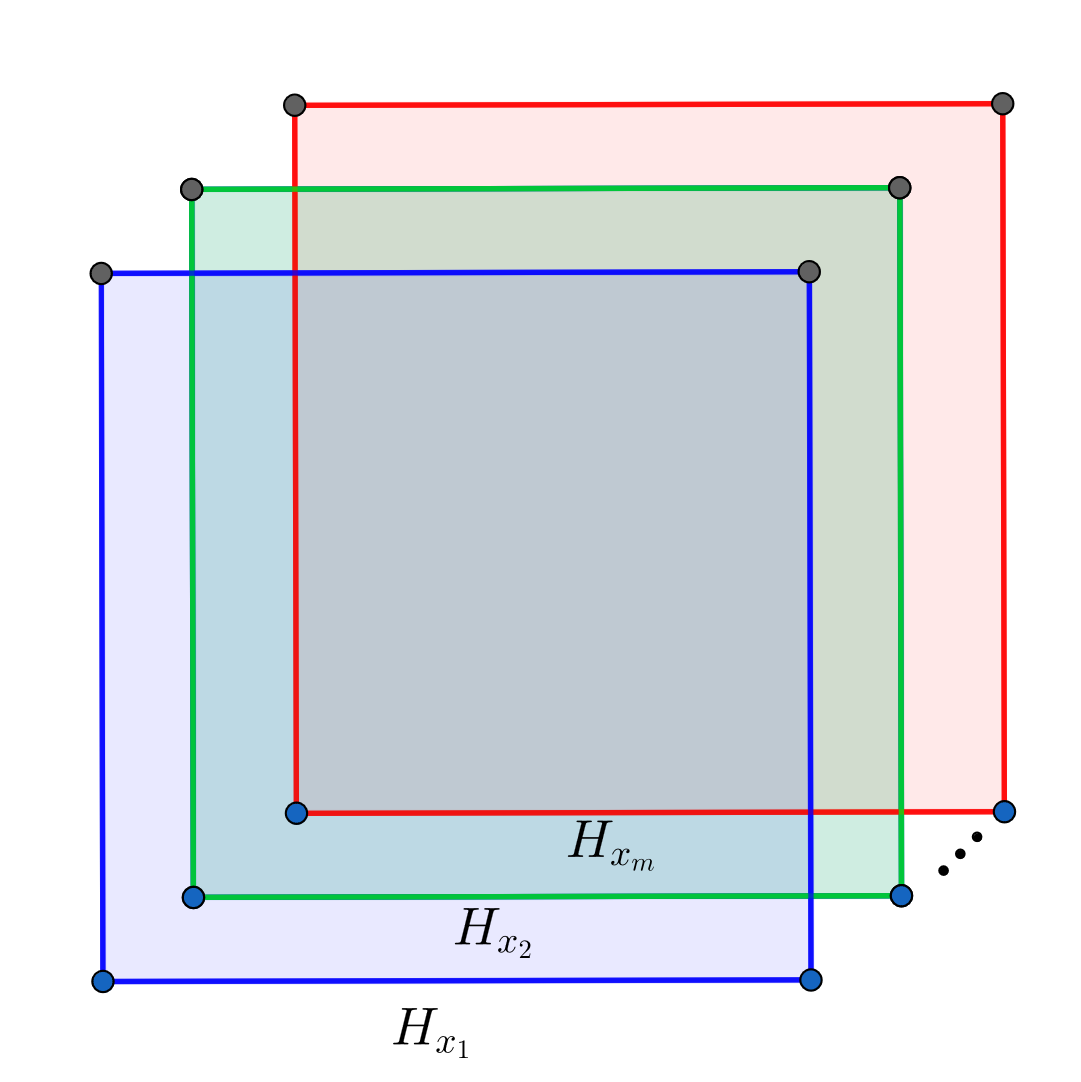
\includegraphics[width=0.4\textwidth, keepaspectratio]{Trajectory_Tensor_1}}
		\subfigure{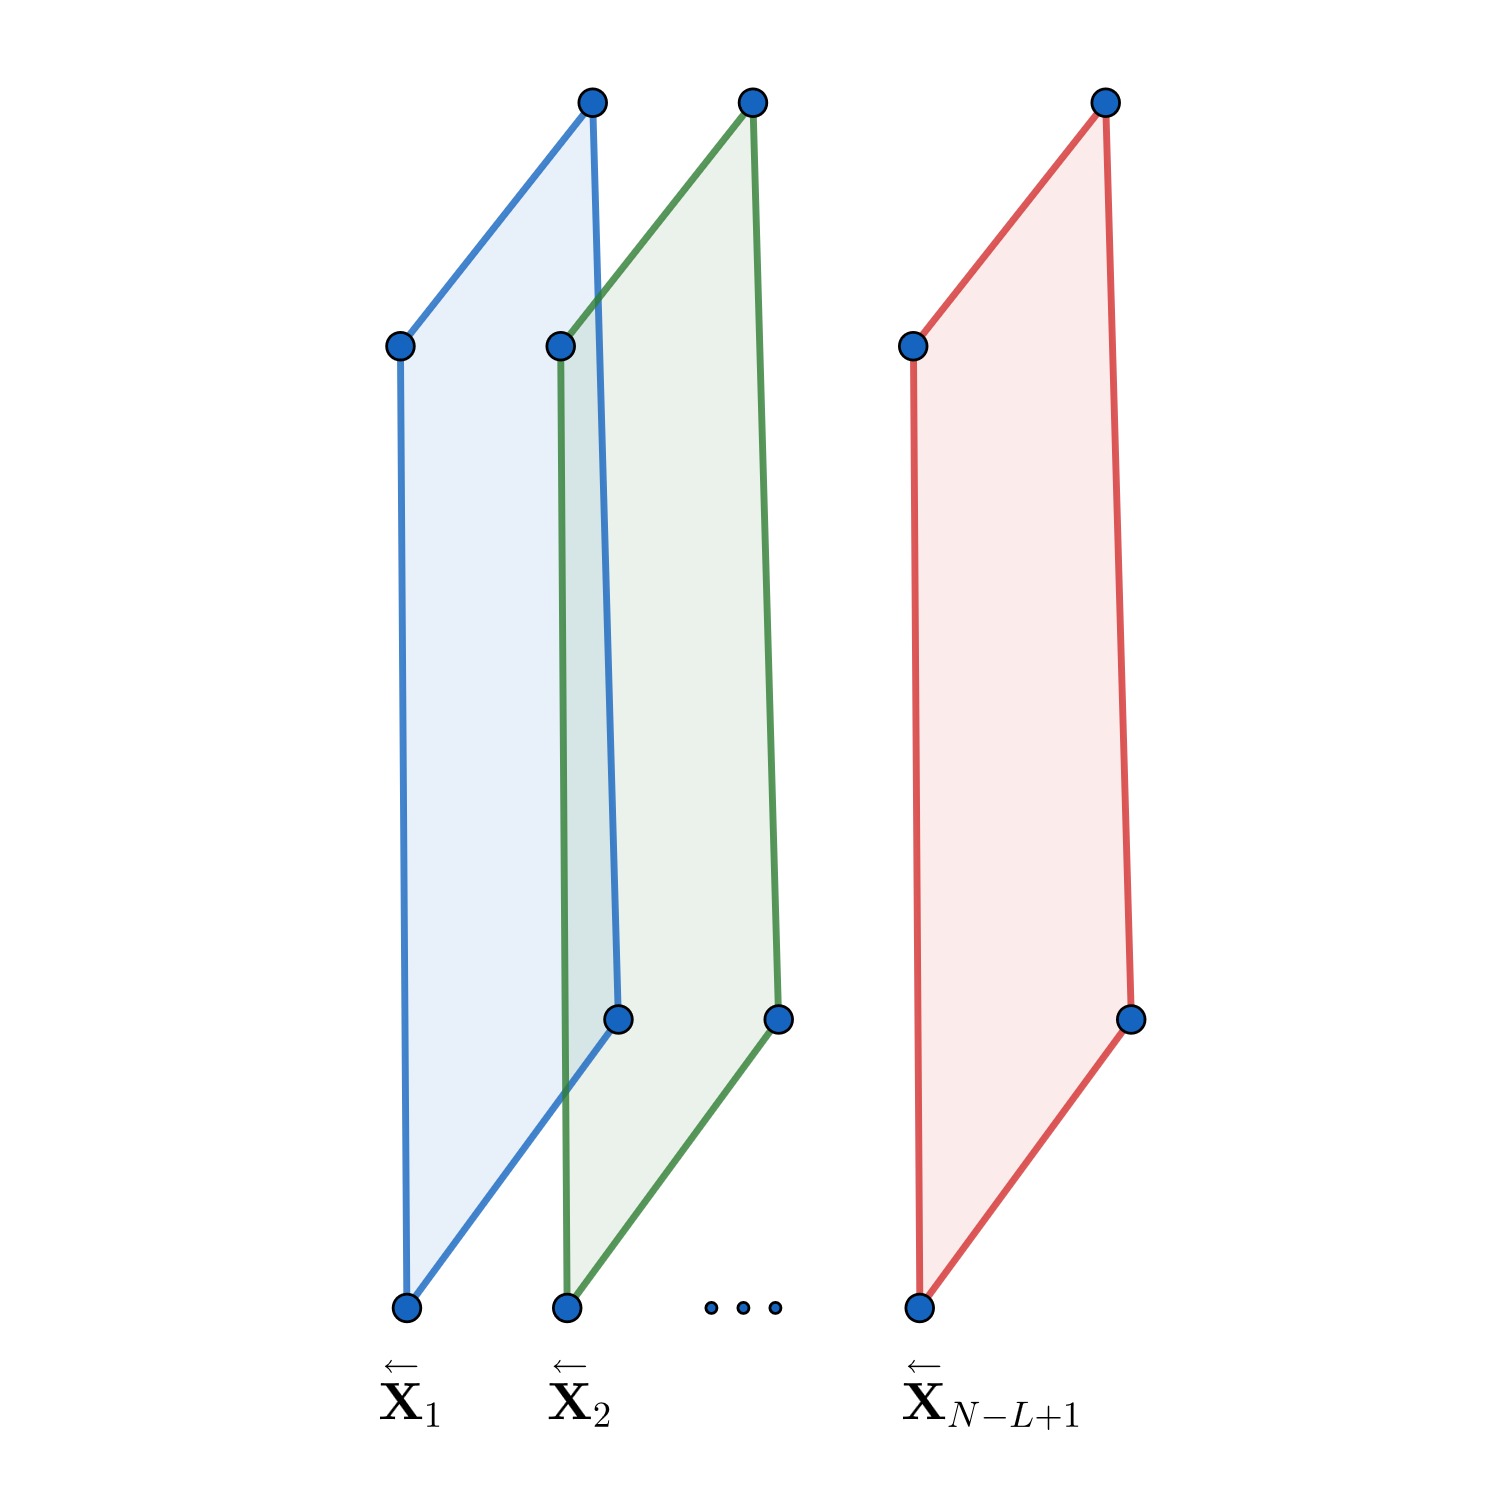
\includegraphics[width=0.4\textwidth, keepaspectratio]{Trajectory_Tensor_2}}
		
		\caption{Two views on trajectory tensor. The left is in terms of signals' trajectory matrices $ \{x_i(t)\}_{i=1}^m $. The right is in terms of delay matrices.}\label{pic:traj_tensor}
	\end{figure}
	
	Similarly to the trajectory matrix introduce the \textit{trajectory tensor} denoted by $ \mathbf{T} $. It stacks delay matrices along the second index of the tensor, Fig.~\ref{pic:traj_tensor} (left). From the definition it follows that each tensor slice along the second index is the trajectory matrix. Then, the $ \mathbf{T} $ is also the trajectory matrices $ H_{x_i} $ stacked along the third index, Fig.~\ref{pic:traj_tensor} (right). Therefore, the shared phase space of the series is equal to a linear span of all $ H_{x_i} $. As discussed in the Sec~\ref{sec:one_series}, each trajectory matrix also defines the individual phase space for the corresponding time series $ x_i(t) $. Finally, we give a 
	
	\begin{Def}\label{def:interdepend}	
		The multivariate time series are said to be \emph{interdependent} if they share the common phase space with the same basis.
	\end{Def}
	
	Assuming the observed series interdependence, it follows that each $ H_{x_i} $ has a matrix factorization with the same set of factors. Since the trajectory matrices constructs the trajectory tensor, it has a low-dimensional representation. Using these two corollaries, we apply the CP-decomposition to the $ \mathbf{T} $ and obtain
	
	\begin{equation}\label{eq:CPD}
		\mathbf{T} = \sum\limits_{i = 1}^{r} \mathbf{a}_i \otimes \mathbf{b}_i \otimes \mathbf{c}_i .
	\end{equation}
	The CPD is defined by the tensor rank $ r $ and a set of vectors. The vectors are usually composed in full-rank matrices 
	
	\begin{equation}\label{eq:cpd_matrices}
		A = [\mathbf{a}_1 \ldots \mathbf{a}_r], B = [\mathbf{b}_1 \ldots \mathbf{b}_r], C = [\mathbf{c}_1 \ldots \mathbf{c}_r] .
	\end{equation}
	Denote by $ \boldsymbol{\sigma}_{x_k} $ the $ k $-th row of the $ C $. Finally, with respect to the third-dimension slices of the $ \mathbf{T} $, CPD goes as
	
	\begin{equation}\label{eq:tSSA_decomp}
		\begin{cases}
			H_{x_1} = \sum\limits_{i = 1}^{r} \boldsymbol{\sigma}_{x_1}(i) \cdot \mathbf{a}_i  \mathbf{b}_i^{\mathsf{T}},  \\
			H_{x_2} = \sum\limits_{i = 1}^{r} \boldsymbol{\sigma}_{x_2}(i) \cdot \mathbf{a}_i  \mathbf{b}_i^{\mathsf{T}}, \\
			\ldots \\
			H_{x_m} = \sum\limits_{i = 1}^{r} \boldsymbol{\sigma}_{x_m}(i) \cdot \mathbf{a}_i  \mathbf{b}_i^{\mathsf{T}} .
		\end{cases}
	\end{equation}
	
	The CPD exists for any tensor. In case of the trajectory tensor three properties must hold.
	
	\begin{Th}\label{th:cpd_phase}
		Suppose that the given multivariate time series are interdependent. Then
		
		\begin{enumerate}
			\item Any $ \boldsymbol{\sigma}_{x_k} $ is a non-zero vector.
			\item The tensor rank $ r \le L $. It is equal to the dimension of the shared phase space.
			\item Transposition of the trajectory matrix is a a trajectory matrix. The shared phase space for the transposed matrices is the $ \text{Lin}(\{\mathbf{b}_i\}) $.
		\end{enumerate}
	\end{Th}
	
	\begin{proof}
		\begin{enumerate}
			\item Suppose some vector has a zero element at the position $ j $ and the other is non-zero in this position. Then two trajectory matrices factorize with a different set of factors. That violates the definition of the series interdependence. The other case is that all $ \boldsymbol{\sigma}_{x_k} $ have a zero element at the position $ j $. Then the matrix $ C $ has a zero row and is not full-ranked. It contradicts to the CPD definition.
			\item Since delay vectors are $ L $-dimensional, each time series has its phase space dimension $ \le L $. All delay vectors of every series also lie in the shared phase space $ \text{Lin}(\{\mathbf{a}_i\}) $. Therefore, dimensionality of the shared space can not be greater than $ L $. Then, the set of $ \{\mathbf{a}_i\}_{i=1}^r $ vectors is linear-independent as follows from the CPD definition. So the dimension of the shared phase space equals $ r $.
			\item Rows of the trajectory matrices are the delay vectors of size $ N - L + 1 $. Transpose all equalities in the (\ref{eq:tSSA_decomp}). Now it is clear that rows of any $ H_{x_i} $ belongs to the $ \text{Lin}(\{\mathbf{b}_i\}) $. This is the shared phase space for the new delay vectors.
		\end{enumerate}
	\end{proof}

	\section{Time series decomposition}\label{sec:decomposition}
	
	The series are decomposed into additive components using the following conception: \emph{factorization of the trajectory matrix $ H_{x_k} $ defines the decomposition of the related time series}. This idea comes from the SSA method. Since all $ H_{x_k} $ have a similar factorization, each time series is decomposed separately.
	
	Trajectory matrices of the series are \emph{hankel} by their definition. That means equal elements along each anti-diagonal of the matrix. It is trivial that any time series of length $ N $ bijectionly corresponds to a hankel matrix of size $ L \times (N - L + 1) $.
	
	Describe the decomposition algorithm. First, the factors of the $ H_{x_k} $ are arbitrary partitioned into $ s $ groups. The $ s $ is also a chosen number. Then all factors within each partition are summed up. As a result we obtain matrices $ C_1, \ldots, C_s $. If they are all hankel then each $ C $ matrix corresponds to the time series component of the $ x_i(t) $. However, it is almost infeasible even with the trivial series (see the \cite{ecfb9dc578be43ae9ee8fc88b8ff9151}). Therefore every $ C $ matrix is additionally \emph{hankelized}. This operator averages each matrix's anti-diagonals so the matrix becomes hankel. Denote it as $ \text{Hankel}(\cdot) $. Finally, the algorithm can be written as a chain of identical transformations
	
	\begin{gather}
		H_{x_k} = \\
		\sum\limits_{i = 1}^{r} \boldsymbol{\sigma}_{x_k}(i) \cdot \mathbf{a}_i  \mathbf{b}_i^{\mathsf{T}} = \label{eq:decomp_alg_first_step} \\
		\sum\limits_{i \in \mathbb{I}_1} \boldsymbol{\sigma}_{x_k}(i) \cdot \mathbf{a}_i  \mathbf{b}_i^{\mathsf{T}} + \ldots + \sum\limits_{i \in \mathbb{I}_s} \boldsymbol{\sigma}_{x_k}(i) \cdot \mathbf{a}_i  \mathbf{b}_i^{\mathsf{T}} = \\
		C_1 + \ldots + C_s = \label{eq:hankelization_step} \\
	    \text{Hankel}(C_1) + \ldots + \text{Hankel}(C_s). \nonumber \\
	    \text{Final expression corresponds to the } x_k(t) = c_1(t) + \ldots c_s(t). \nonumber
	\end{gather}
    
	Here $ \mathbb{I}_1 \sqcup \ldots \sqcup \mathbb{I}_s = \{1, \ldots, r\} $ are chosen groups of indices. $ c_1(t), \ldots , c_s(t) $ are the time series extracted from the $ \text{Hankel}(C_1), \ldots , \text{Hankel}(C_s) $ (see the second paragraph of this section). The (\ref{eq:hankelization_step}) step requires a proof. But first, consider a hankel operator's property:
	
	\begin{Lem}
		The $ \text{Hankel}(\cdot) $ is a linear operator.
	\end{Lem}
	
	\begin{proof}		
		Having matrices $ A $ and $ B $ with the same size, take their elements from any anti-diagonal. Denote them by $ a_1, \ldots, a_n $ and $ b_1, \ldots, b_n $. Then this anti-diagonal in $ \text{Hankel}(A + B) $ is
		\begin{equation*}
			 \dfrac{1}{n} \sum\limits^n (a_i + b_i) = \dfrac{1}{n} \sum\limits^n a_i + \dfrac{1}{n} \sum\limits^n b_i.
		\end{equation*}
		It exactly results in a sum of the $ \text{Hankel}(A) $'s and $ \text{Hankel}(B) $'s anti-diagonals.
		
		Secondly, having the scalar $ \alpha $, it is trivial that 
		\begin{equation*}
			 \dfrac{1}{n} \sum\limits^n \alpha \cdot a_i = \alpha \dfrac{1}{n} \sum\limits^n a_i.
		\end{equation*}
		Hence, we derive $ \text{Hankel}(\alpha A) = \alpha \text{Hankel}(A) $.
	\end{proof}
	
	Now recall that the $ H_{x_k} $ is hankel. Combining it with the previous lemma, apply $ \text{Hankel}(\cdot) $ to the $ H_{x_k} = C_1 + \ldots + C_s $ from the algorithm. This proofs the (\ref{eq:hankelization_step}). Therefore, we have shown the correctness of the decomposition algorithm.
	
	\section{Optimal decomposition problem}\label{sec:optimal_decomp}
	
	To eliminate ambiguity in the partitioning of the $ H_{x_k} $ factors, we restrict $ C_j $ matrices to be hankel. Thus, the (\ref{eq:hankelization_step}) step of the decomposition algorithm becomes unnecessary. In addition, such partitioning completely fulfills the decomposition concept. 
	
	Formulate the decomposition problem as a system of matrix equations. Take the (\ref{eq:decomp_alg_first_step}) equality and apply the hankel operator to both sides. Recall that the $ H_{x_k} $ is hankel. Also take the very same equality as it is. We obtain
	\begin{equation*}
		\begin{cases*}
			H_{x_k} = \sum\limits_{i = 1}^{r} \boldsymbol{\sigma}_{x_k}(i) \cdot \mathbf{a}_i  \mathbf{b}_i^{\mathsf{T}}, \\
			H_{x_k} = \sum\limits_{i = 1}^{r} \text{Hankel}(\boldsymbol{\sigma}_{x_k}(i) \cdot \mathbf{a}_i  \mathbf{b}_i^{\mathsf{T}}).
		\end{cases*}
	\end{equation*}
	Then, subtract the second from the first and introduce
	\begin{equation*}
		H_i = \boldsymbol{\sigma}_{x_k}(i) \cdot \mathbf{a}_i  \mathbf{b}_i^{\mathsf{T}} - Hankel(\boldsymbol{\sigma}_{x_k}(i) \cdot \mathbf{a}_i  \mathbf{b}_i^{\mathsf{T}})
	\end{equation*}
	It is called the \emph{hankel residual matrix} of the $ i $-th factor. Therefore we get \begin{equation}\label{eq:residuals_equation}
		H_1 + \ldots + H_r = 0. \quad \text{Or equally } H_r = - \sum\limits_{j = 1}^{r - 1} H_j.
	\end{equation}
	The condition on the $ C_i $ to be hankel is reformulated as the residual matrices sum up to zero within each partition group. The problem is to find the non-intersecting sets $ \mathbb{I}_1, \ldots , \mathbb{I}_s $ such that
	
	\begin{gather}\label{eq:decomp_opt_init}
		\sum_{k \in \mathbb{I}_i} H_k = 0, \ i \in 1, \ldots, s , \\
		\mathbb{I}_1 \sqcup \ldots \sqcup \mathbb{I}_s = \{1, \ldots, r\} . \nonumber
	\end{gather}
	
	Without loss of generality, we set $ s $ equals two. Only $ \mathbb{I}_1, \mathbb{I}_2 $ must be found. If (~\ref{eq:decomp_opt_init}~) is solved in such setting, then $ \mathbb{I}_1 $ and $ \mathbb{I}_2 $ can be further partitioned separately. Hence, any number of the time series components can be obtained. Moreover, for any $ H_{x_k} $ its residual matrices are linearly dependent as follows from the (\ref{eq:residuals_equation}). Thus, the partition group for the $ H_r $ is uniquely defined if all other residuals are already partitioned. This matrix can be discarded. We also assume all $ H_j $ to be non-zero matrices. Otherwise, the zero residual matrix alone and all the rest make the desired partition on two groups. This assumption implies each of the groups to have at least two residual matrices. Finally, for any $ H_j $ matrix introduce an indicator-variable $ \beta_j \in \{0, 1\} $. It shows what group the residual matrix belongs to. Denote by $ \boldsymbol{\beta} $ a vector $ [\beta_1 \ldots \beta_{r-1}]^{\text{T}} $. The decomposition problem is to find $ \boldsymbol{\beta} $ such that
	
	\begin{equation}\label{eq:first_optimal_decomp}
		\begin{cases*}
			\sum\limits_{j = 1}^{r - 1} \beta_j H_j = 0, \\
			\beta_j \in \{0, 1\} \ \forall j \in 1 \ldots r, \\
			\sum\limits_{i = 1}^{r - 1} \beta_j \ge 2.
		\end{cases*}
	\end{equation}
	
	The \cite{ecfb9dc578be43ae9ee8fc88b8ff9151} shows that even for trivial time series such a problem is infeasible. Now we transform it into a feasible one. First, vectorize each $ H_i $ and stack resulting vectors into the matrix denoted by $ \Lambda $. Then the first equation in the (\ref{eq:first_optimal_decomp}) is equivalent to the $ \Lambda \boldsymbol{\beta} = 0 $. Second, change the problem of solving the system of equations to an optimization problem. Let's find such $ \boldsymbol{\beta} $ that delivers minimum to the norm of the $ \Lambda \boldsymbol{\beta} $. The changed problem is
	\begin{equation}\label{eq:decomp_search_final}
		\begin{cases*}
			\lVert \Lambda \boldsymbol{\beta} \rVert \to \underset{\boldsymbol{\beta}}{\min}, \\
			\beta_j \in \{0, 1\} \ \forall j \in 1 \ldots r, \\
			\sum\limits_{i = 1}^{r - 1} \beta_j \ge 2.
		\end{cases*}
	\end{equation}
	Call solution of the (\ref{eq:decomp_search_final}) the \emph{optimal series decomposition}. The problem itself is an Integer Least Squares (ILS) problem, which is proved to be NP-hard~\cite{van1981another}. Therefore, \emph{the optimal series decomposition is an NP-hard problem}.
	
	In spite of the complexity, methods and heuristics exist to reduce the ILS to computationally effective problems, see \cite{Grafarend2022}.
	
	\section{Time series forecasting}\label{sec:tssa_forecast}
	
	Using the build shared phase space each time series is forecast individually. We make a one-step forecast to estimate $ x(N + 1) $. Phase trajectory of the series is a sequence of the delay vectors $ \{ \delayV{t} \} $. The whole trajectory belongs to the phase space $ \text{Lin}(\{\mathbf{a}_i\}) $. Continuation of the trajectory is the $ \delayV{N + 1} $. Therefore $ \delayV{N + 1} \in \text{Lin}(\{\mathbf{a}_i\}) $. At the same time $ x(N + 1) $ is the last component of the $ \delayV{N + 1} $. Now, recall the $ A $ matrix from the (\ref{eq:cpd_matrices}). The system of linear equation to find $ x(N + 1) $ is
	
	\begin{align}\label{eq:main_pred_for_A}
		\delayV{N + 1} = A \boldsymbol{\lambda} \text{ or equally } &\begin{cases}
			\mathbf{x} = \tilde{A} \boldsymbol{\lambda}  \\
			x(N + 1) = \mathbf{a}^{\mathsf{T}} \boldsymbol{\lambda}
		\end{cases}, \text{ where } \\
		A &= \left( \dfrac{\tilde{A}}{\mathbf{a}^{\mathsf{T}}} \right), \label{eq:A_split} \\
		\delayV{N + 1} &= (\mathbf{x} \  x(N + 1))^{\mathsf{T}}. \label{eq:del_vec_split}
	\end{align}
	
	The delay vector $ \delayV{N + 1} $ and the matrix $ A $ are split into two blocks, see (\ref{eq:A_split}) and (\ref{eq:del_vec_split}). The blocks are associated with the known and predicted part of the series. The forecast comes from the second equation in the~(\ref{eq:main_pred_for_A}). Therefore, the vector $ \boldsymbol{\lambda} \in \mathbb{R}^r $ is to be found from the first equation in the (\ref{eq:main_pred_for_A}). It is a system of linear equations with the matrix $ \tilde{A} $. The matrix has a rank at least $ r - 1 $ since $ A $ matrix is full-ranked. However, we assume $ \tilde{A} $ to have rank $ r $, too. As experiments show this is not burdensome. In addition, the linear system is overdetermined since $ r \le L $, see  Sec~\ref{sec:tssa_method}. Therefore its solution is given by the least-squares formula $ \boldsymbol{\lambda} = (\tilde{A}^{\mathsf{T}} \tilde{A})^{-1} \tilde{A}^{\mathsf{T}} \mathbf{x} $. After replacing it in (\ref{eq:main_pred_for_A}) we obtain the forecast
	
	\begin{equation}\label{eq:tssa_pred}
		x(N + 1) = \mathbf{a}^{\mathsf{T}} (\tilde{A}^{\mathsf{T}} \tilde{A})^{-1} \tilde{A}^{\mathsf{T}} \mathbf{x}.
	\end{equation}
	
	Denote by $ \mathbf{d} $ the vector $ \mathbf{a}^{\mathsf{T}} (\tilde{A}^{\mathsf{T}} \tilde{A})^{-1} \tilde{A}^{\mathsf{T}} $. Once computed, it is used to make the forecast for further steps. Rewrite the (\ref{eq:tssa_pred}) in terms of $ x(t) $:
	
	\begin{equation*}\label{eq:autoregr}
		x(t) = \sum\limits_{i = 1}^{L - 1} d_i \cdot x(t - i)
	\end{equation*}
	This expression reveals the property of the forecast sequence $ \{x(N + i)\} $.
	
	\begin{Th}\label{th:forecast}		
		The model of the tSSA's forecast is \emph{autoregressive} $ AR(L - 1) $. The coefficients $ d_i $ found in the (\ref{eq:tssa_pred}), completely define behavior of the forecast sequence.
	\end{Th}
	
	\section{Computational experiment}	
	
	Analyze forecast and decomposition quality of the tSSA on sample multivariate time series. Also compare the tSSA with the other methods: the mSSA, the VAR, and the RNN. The RNN and VAR methods are able to make the forecast, but do not contain an explicit way of building series decomposition.
	
	To measure quality of the decomposition we introduce special metrics. They are motivated by the corresponding analysis in the Sec~\ref{sec:decomposition}.
	
	\begin{Def}
		The \emph{absolute hankel error} of the matrix $ M $ is 
		
		\[
		\text{AHE} = \lVert M - \text{Hankel}(M) \rVert_F.
		\] 
		
	\end{Def}	
	
	\begin{Def}		
		
		The \emph{relative hankel error} of the matrix $ M $ is 
		
		\[
		\text{RHE} = \frac{\text{AHE}}{\lVert M \rVert_F}.
		\] 		
		
	\end{Def}
	
	The AHE is proportional to the total variance of matrix's anti-diagonals. The RHE is AHE's more interpretable modification. Recall the decomposition algorithm (\ref{eq:decomp_alg_first_step}). It introduced the $ C_i $ matrices corresponded to the $ c_i(t) $ components of the time series $ x(t) $. The~(\ref{eq:decomp_search_final}) is the optimal decomposition problem. It is basically AHE minimizing for the $ C_i $ matrices. Hence, the AHE and the RHE are computed for the $ C_i $ in the further experiments. Denote by $ \overline{\text{RHE}}_{\text{ts}} $ the mean RHE across all $ C_i $ of the time series named "ts". Denote by $ \overline{\text{RHE}} $ the mean $ \overline{\text{RHE}}_{\text{ts}} $ across time series of this computational experiment.
	
	To measure forecast quality for the time series named "ts", use: the \emph{mean squared error} $ \text{MSE}_{\text{ts}} $ and the \emph{mean absolute percentage error} $ \text{MAPE}_{\text{ts}} $. Denote by $ \overline{\text{MSE}} $ and $ \overline{\text{MAPE}} $ the mean $ \text{MSE}_{\text{ts}} $ and $ \text{MAPE}_{\text{ts}} $ across time series of this computational experiment.
	
	Two sample multivariate time series are involved in the experiment. First, the electricity consumption and price, Fig. \ref{fig:electr_data}. Second, the inertial unit measurements~\cite{accelerometryData}: three time series are from an accelerometer and three from a gyroscope, Fig. \ref{fig:motion_data}. The measurements represent walking movements. We assume the multivariate time series have shared phase space, see Def.~\ref{def:interdepend}. For the electricity series it is related to the law of demand and supply. For the inertial unit series it is related to coupled dynamical system describing the motion. The sample series have the length $ 3 \cdot 10^3 $ time ticks. About $ 20\% $ of them are deferred test samples for the forecast quality evaluation.
	
	\begin{figure}[!htbp]
		\centering
		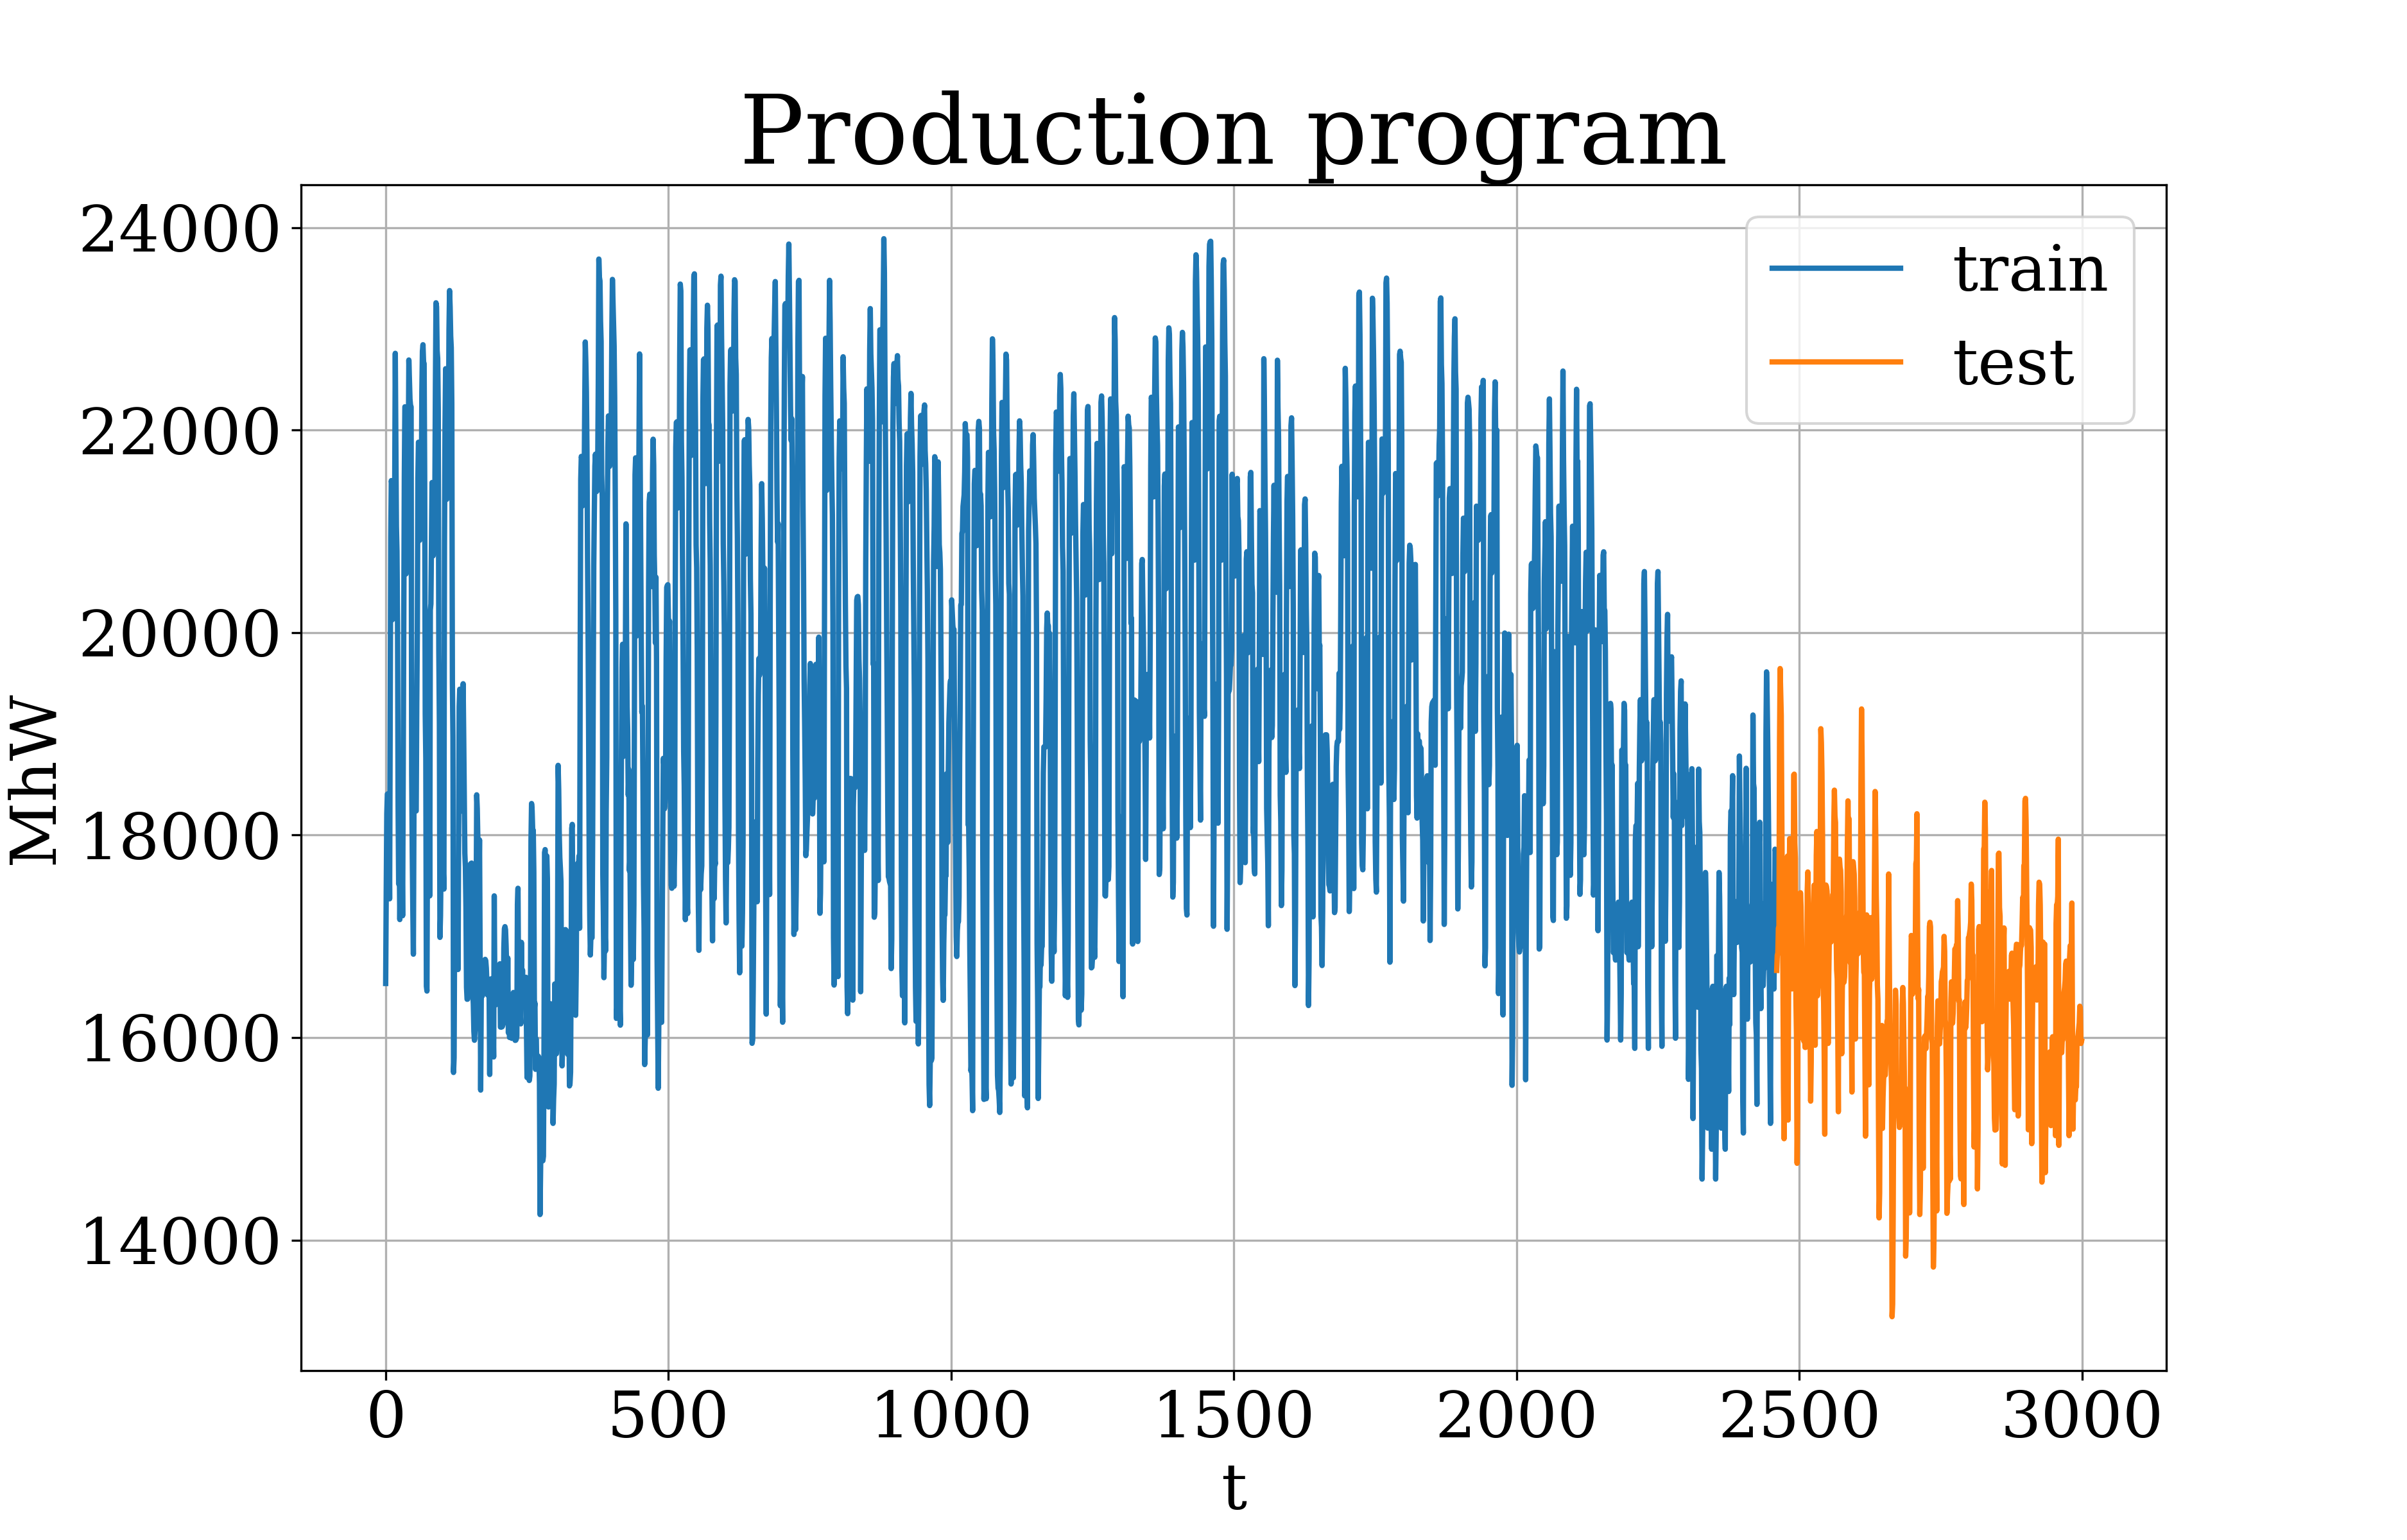
\includegraphics[width=0.48\textwidth, keepaspectratio]{Electricity_Production}
		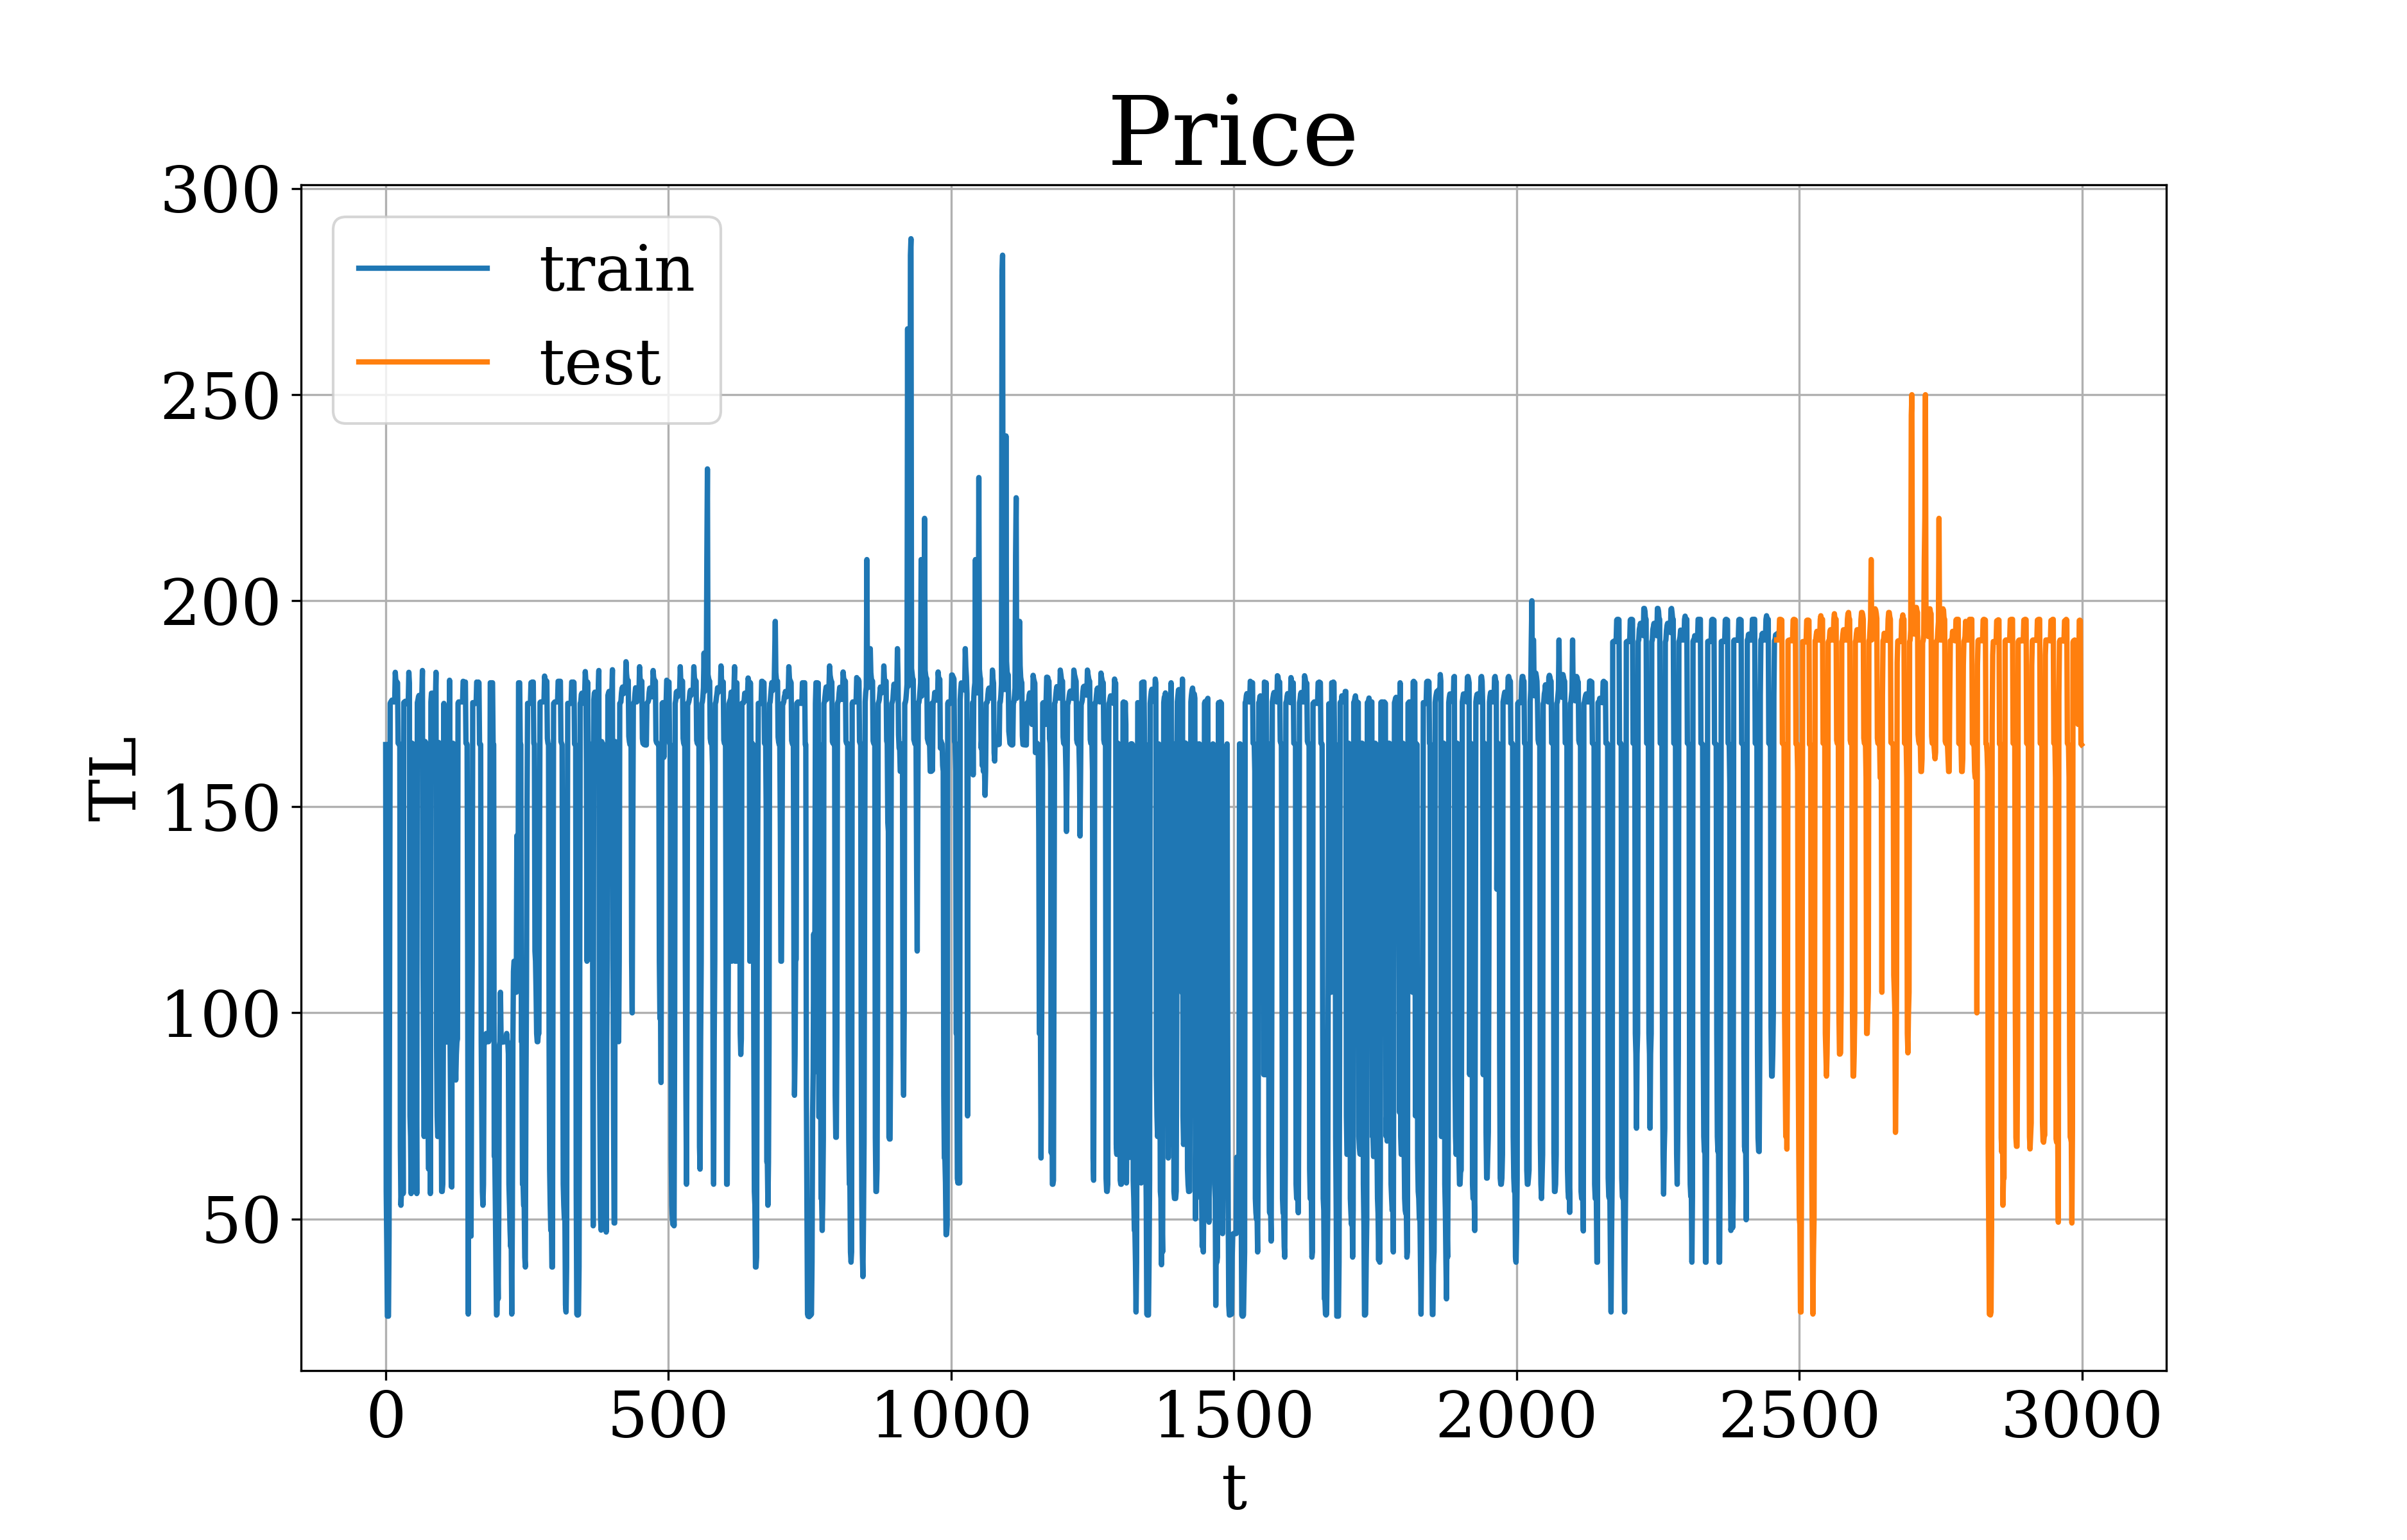
\includegraphics[width=0.48\textwidth, keepaspectratio]{Electricity_Price}
		\caption{Time series for the electricity consumption and price}\label{fig:electr_data}
	\end{figure}
	
	\begin{figure}[!htbp]
		\centering
		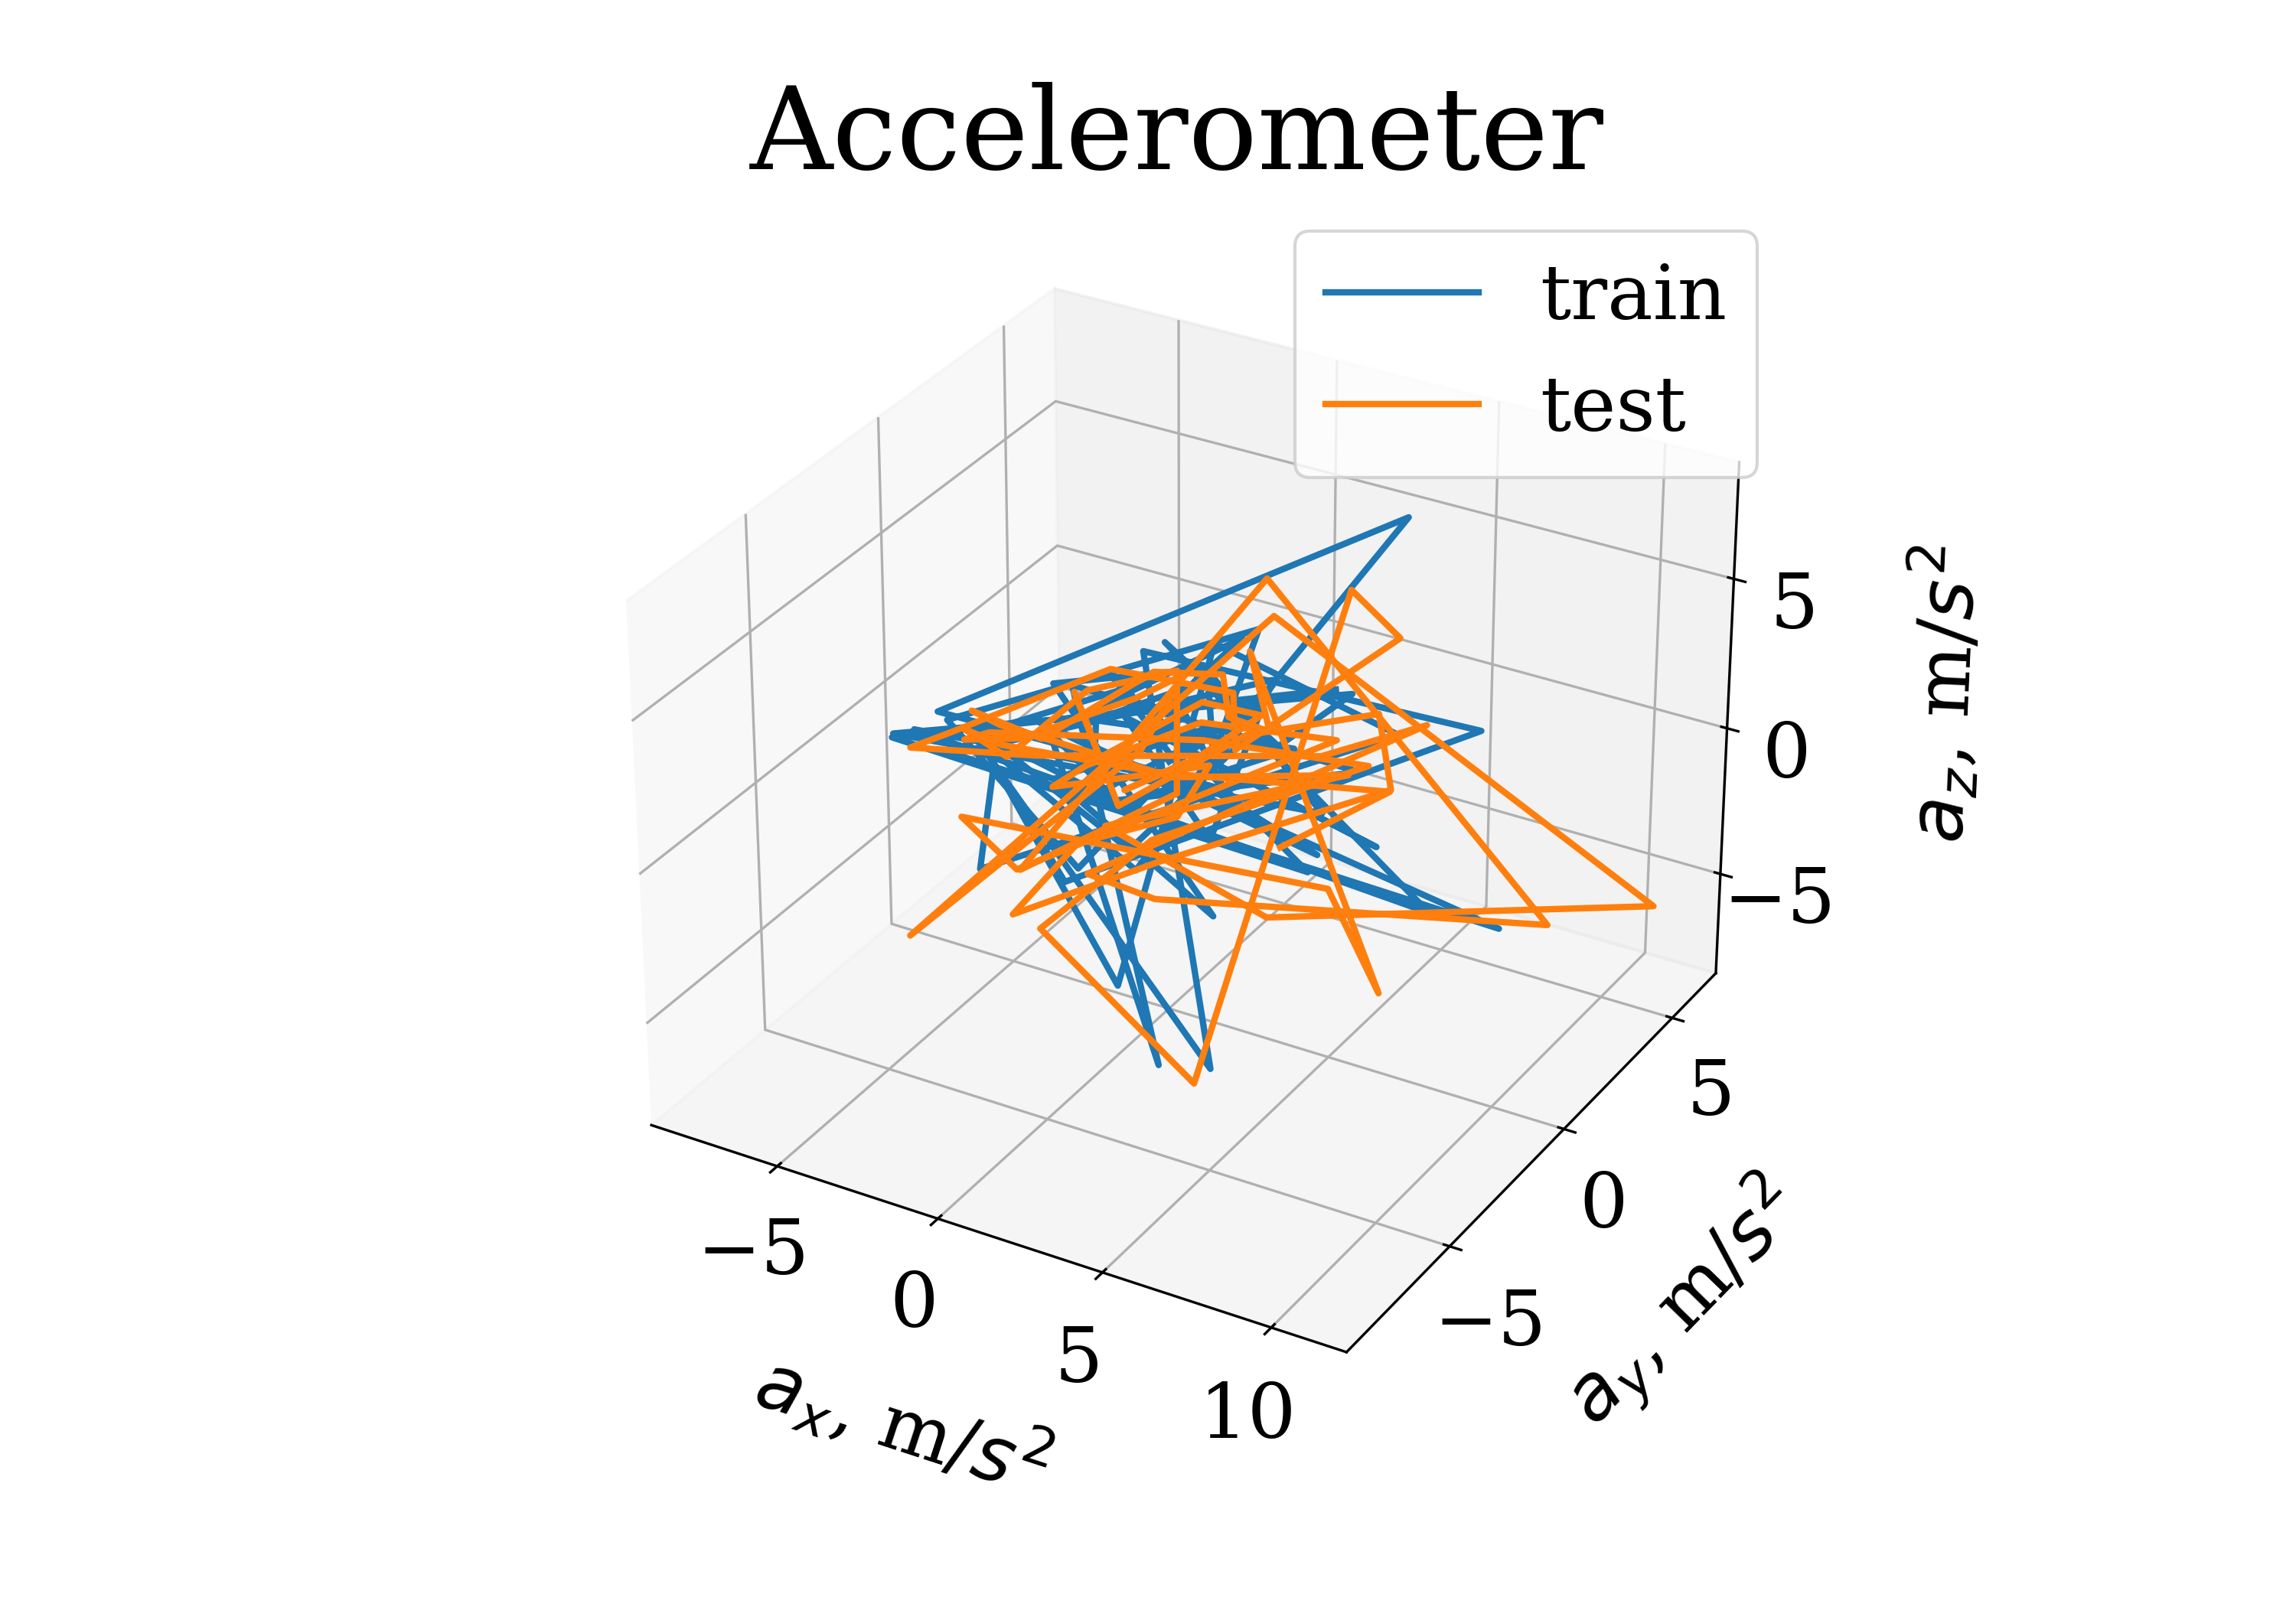
\includegraphics[width=0.48\textwidth, keepaspectratio]{acceleromter_example.png}
		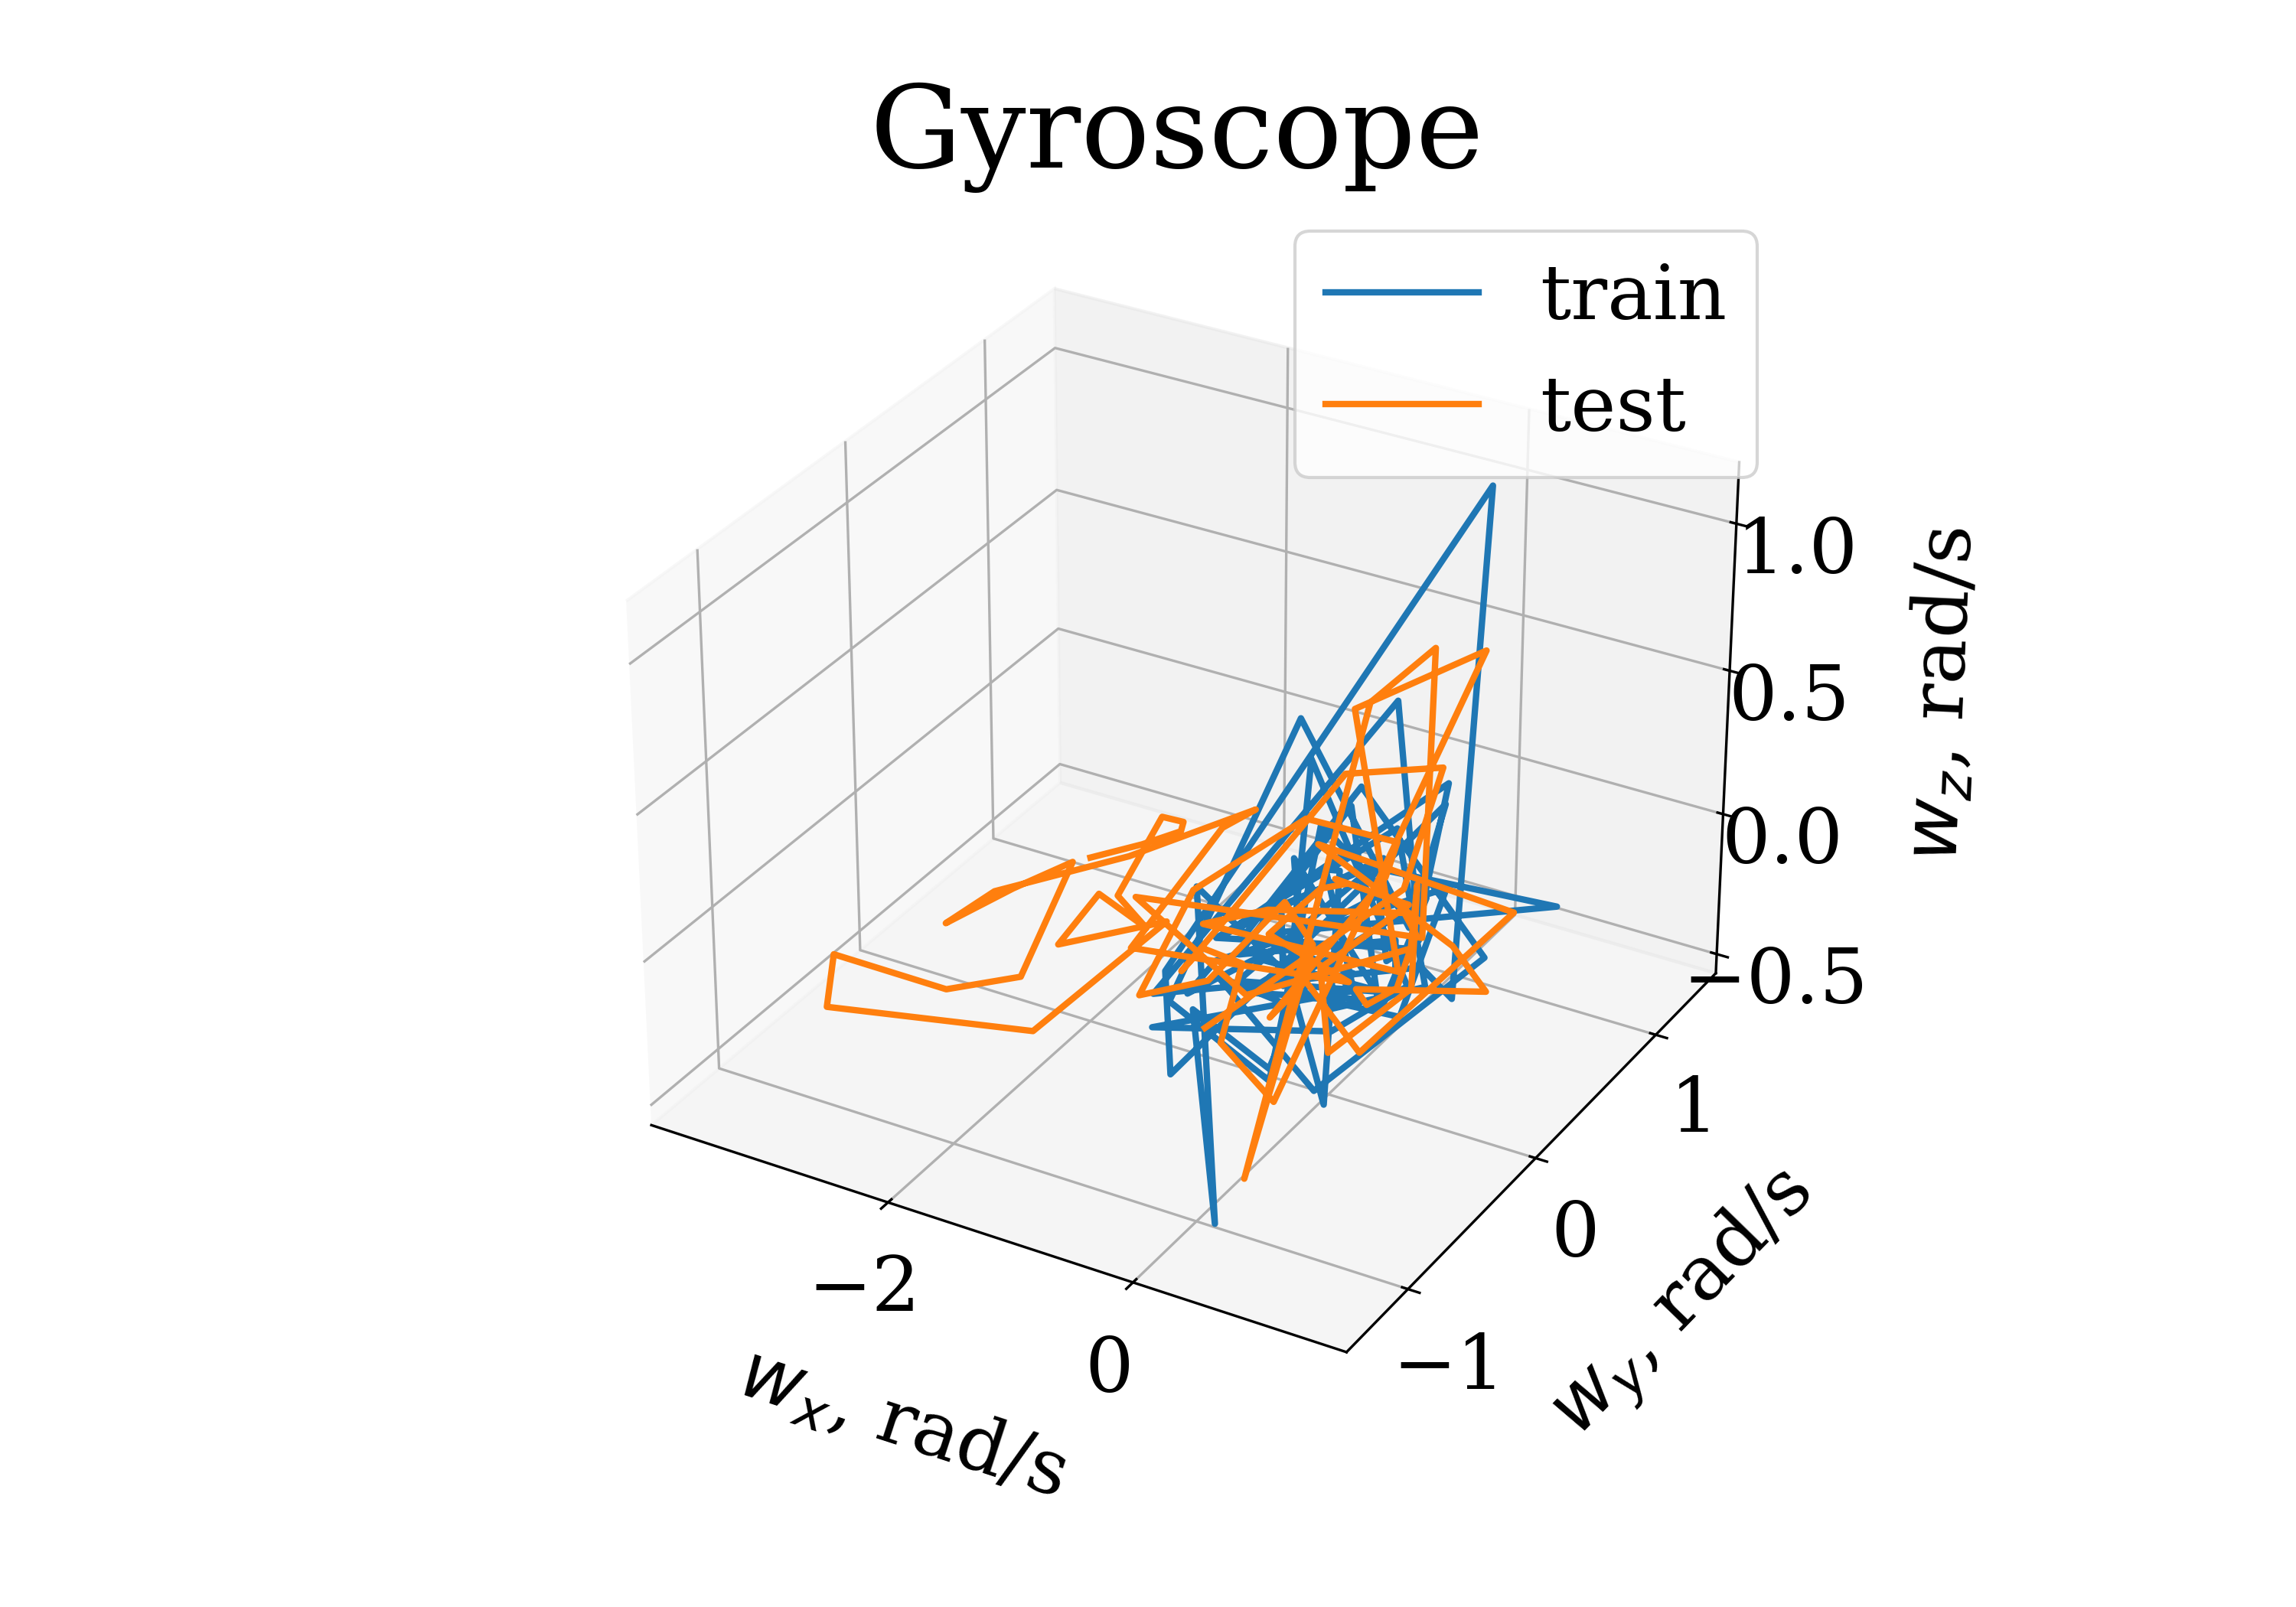
\includegraphics[width=0.48\textwidth, keepaspectratio]{gyro_example.png}
		\caption{Time series for the inertial unit measurements}\label{fig:motion_data}
	\end{figure}
	
	The tSSA's parameter $ L $ is set to $ 500 $ for the electricity series and to $ 1000 $ for the inertial unit series. This is also a parameter for the other models. For the RNN it is the minimum length of series. For the VAR it is a maximal lag number. For the mSSA it is similar to the tSSA.
	
	\section{Data availability}
	
	The electricity consumption data is available at \url{https://sourceforge.net/p/mvr/code/HEAD/tree/data/TurkElectricityConsumption.csv}. The inertial unit data is available at \url{https://data.mendeley.com/datasets/45f952y38r/5}.
	
	\section{Results and discussion}
	
	\paragraph{The forecast}
	
	The trajectory tensor rank is equal to the forecast model's order, see Th.~\ref{th:forecast}. Since efficient computation of tensor rank is impossible, the rank becomes tSSA's parameter. Fig. \ref{fig:mse_mape_electr} and \ref{fig:mse_mape_motion} show the forecast quality decreases with the greater ranks for the MAPE and MSE. Optimal rank value is 30. Nonetheless, the CPD computation error decreases monotonously with greater ranks, see Fig. \ref{fig:cpd_errors}. This error is an estimation of how close the computed CPD is to the true one (\ref{eq:CPD}). As a result, the small-order forecast model delivers the best quality. 

	\begin{figure}[!htbp]
		\centering
		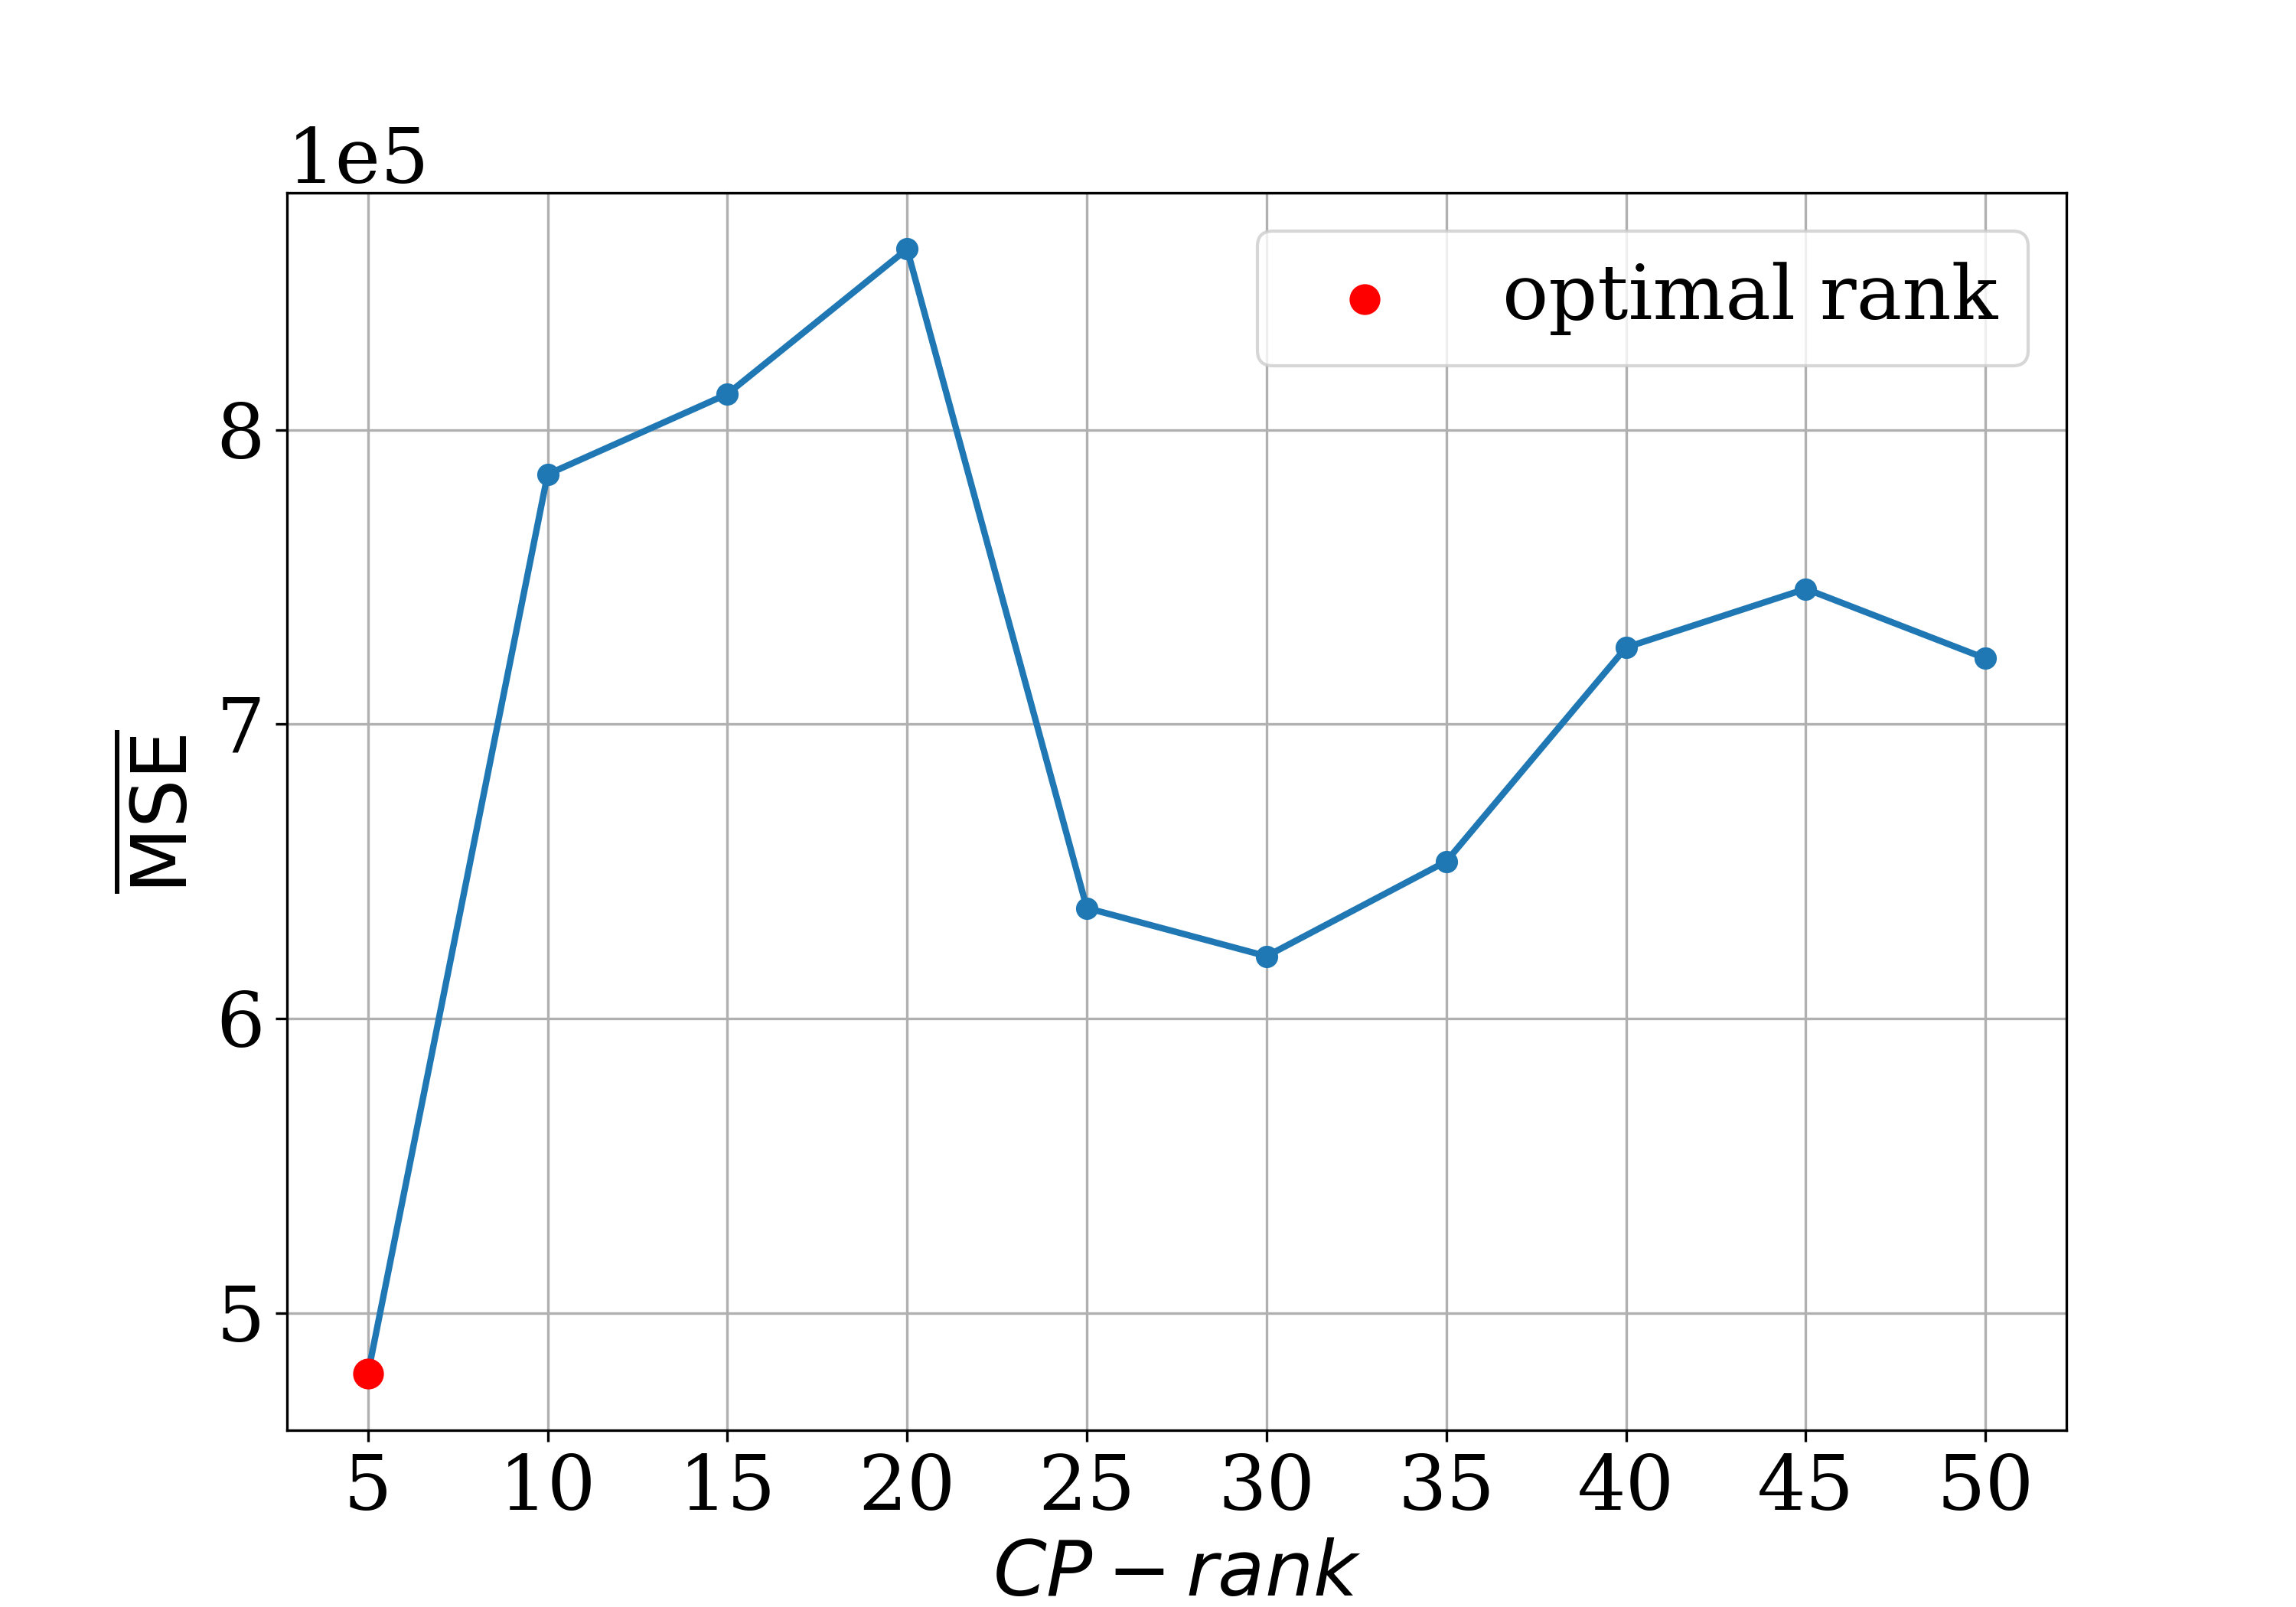
\includegraphics[width=0.48\textwidth, keepaspectratio]{pred_MSE_rank_elec.png}
		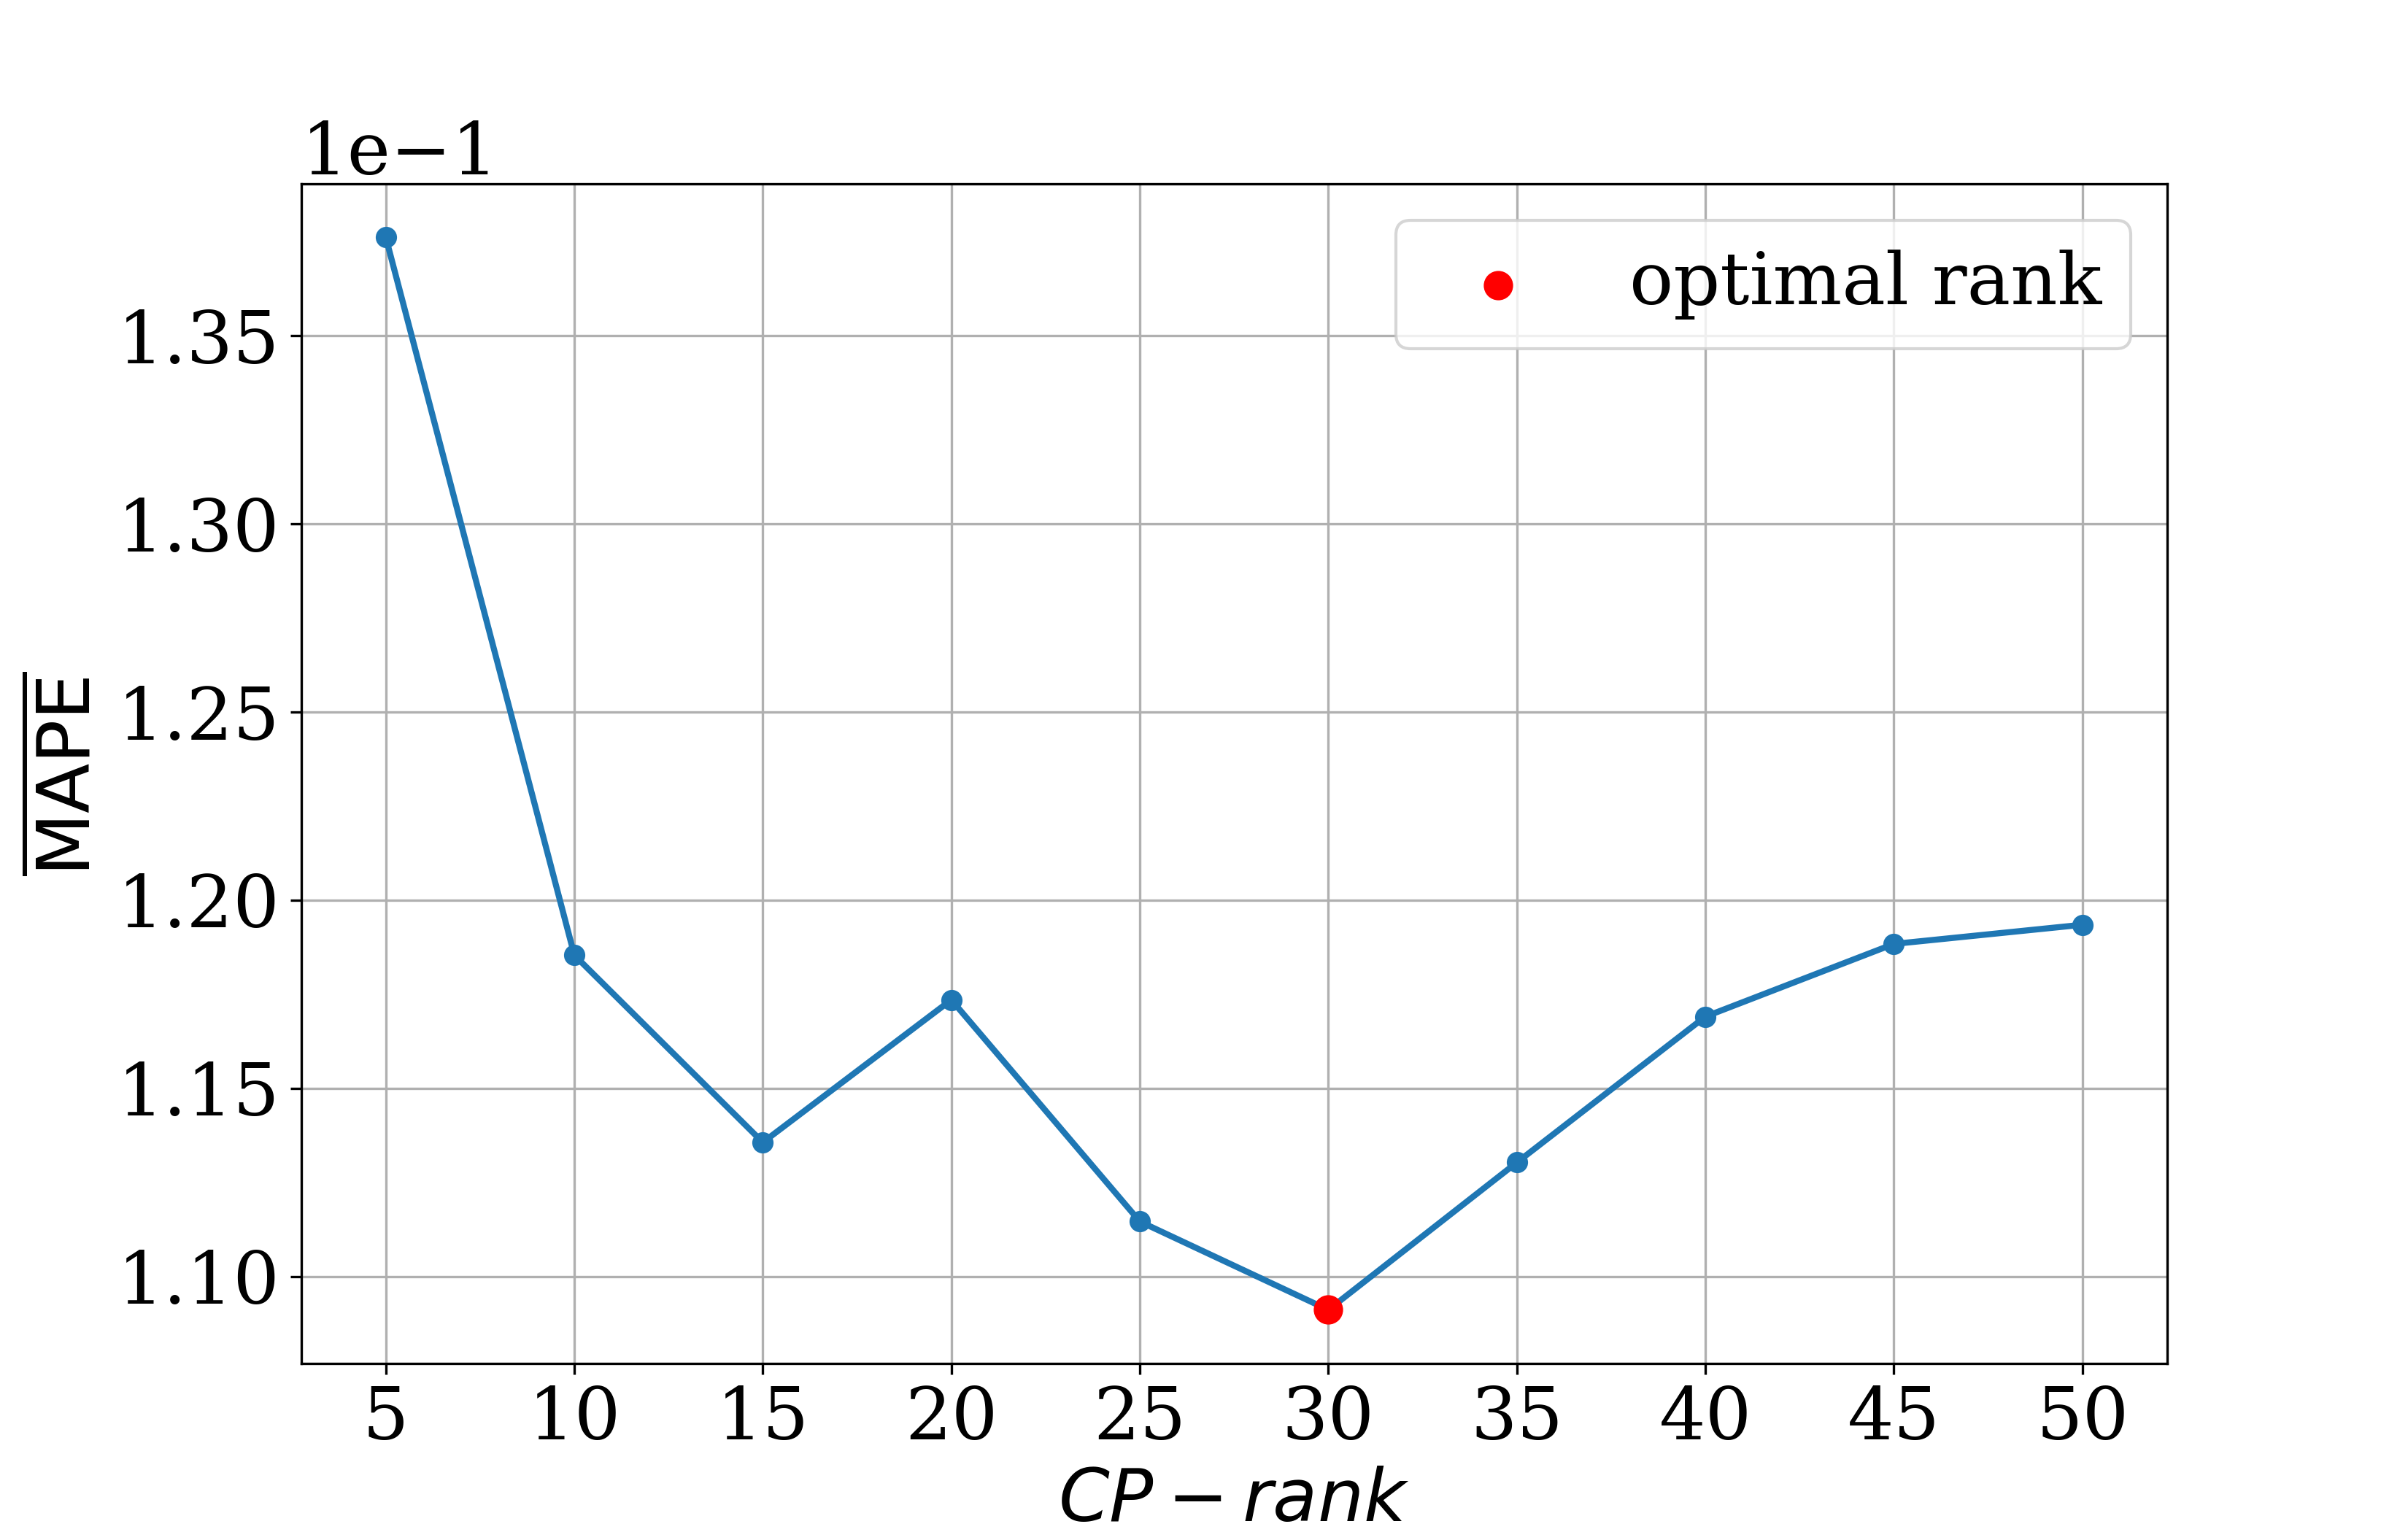
\includegraphics[width=0.48\textwidth, keepaspectratio]{pred_MAPE_rank_elec.png}
		\caption{$ \overline{\text{MSE}} $ and $ \overline{\text{MAPE}} $ metrics for the tSSA forecast depending on the CPD rank. An optimal point is marked with red. Electricity data.}\label{fig:mse_mape_electr}
	\end{figure}
	
	\begin{figure}[!htbp]
		\centering
		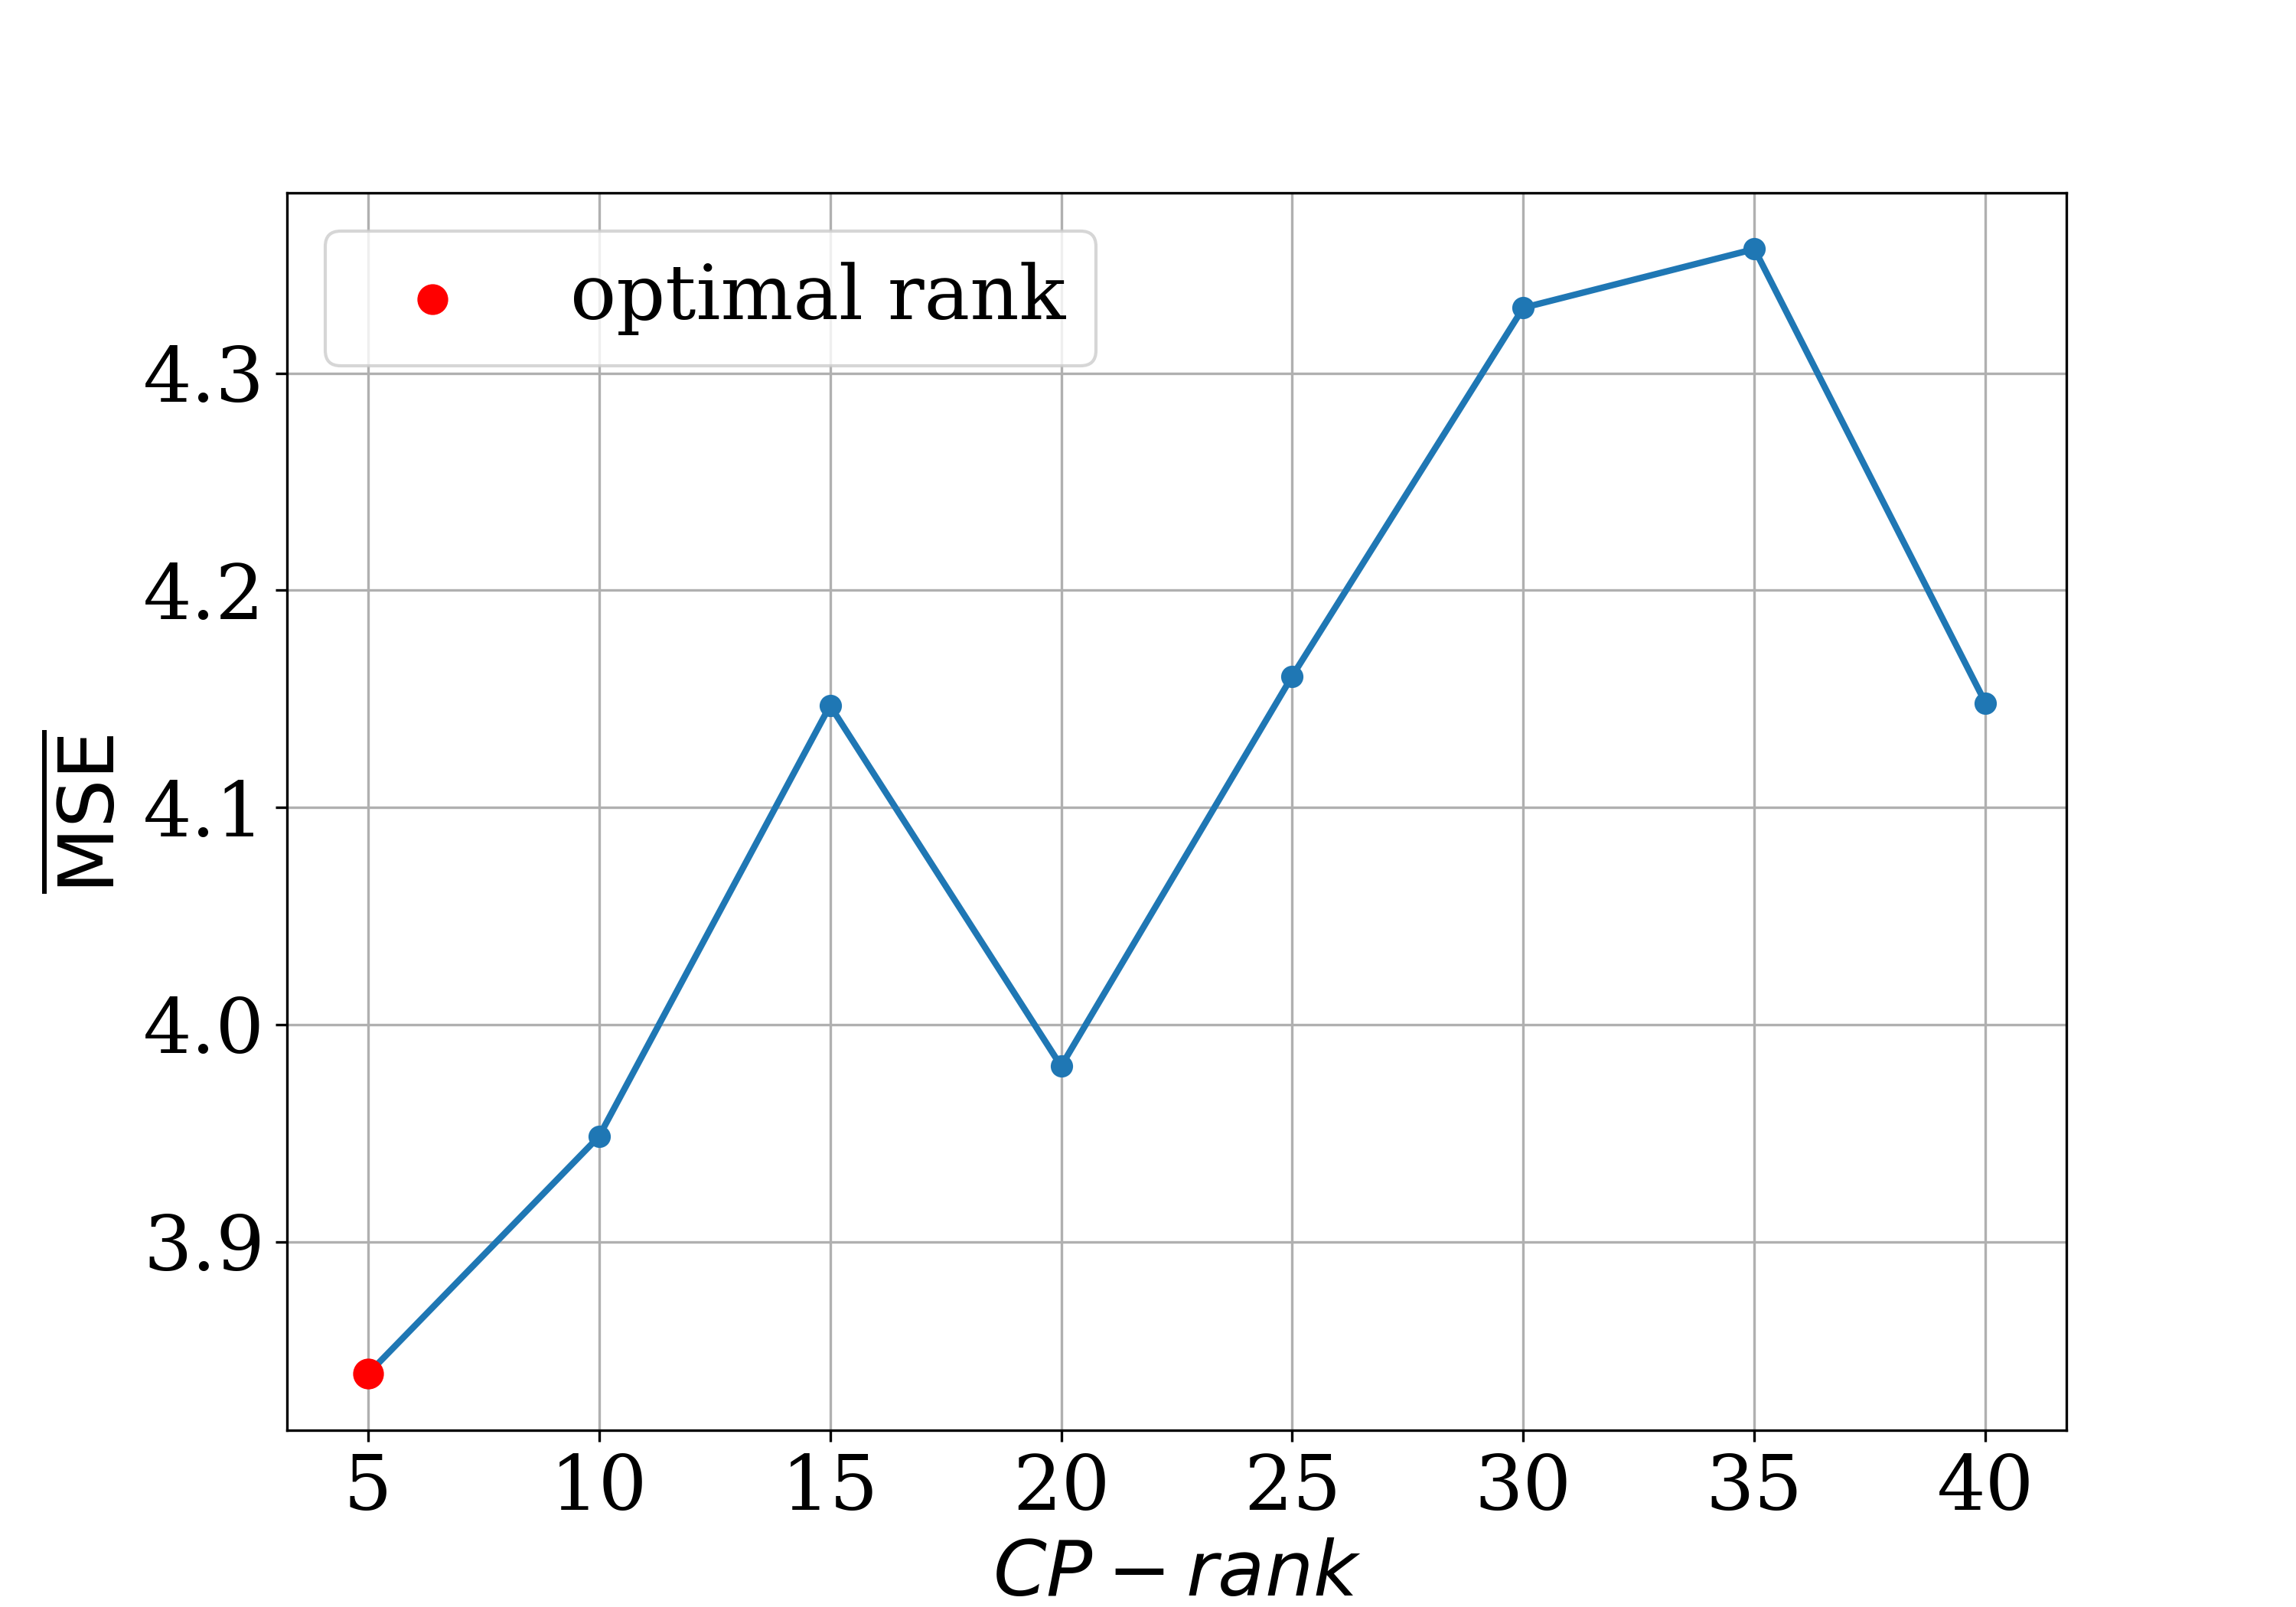
\includegraphics[width=0.48\textwidth, keepaspectratio]{pred_MSE_rank_motion.png}
		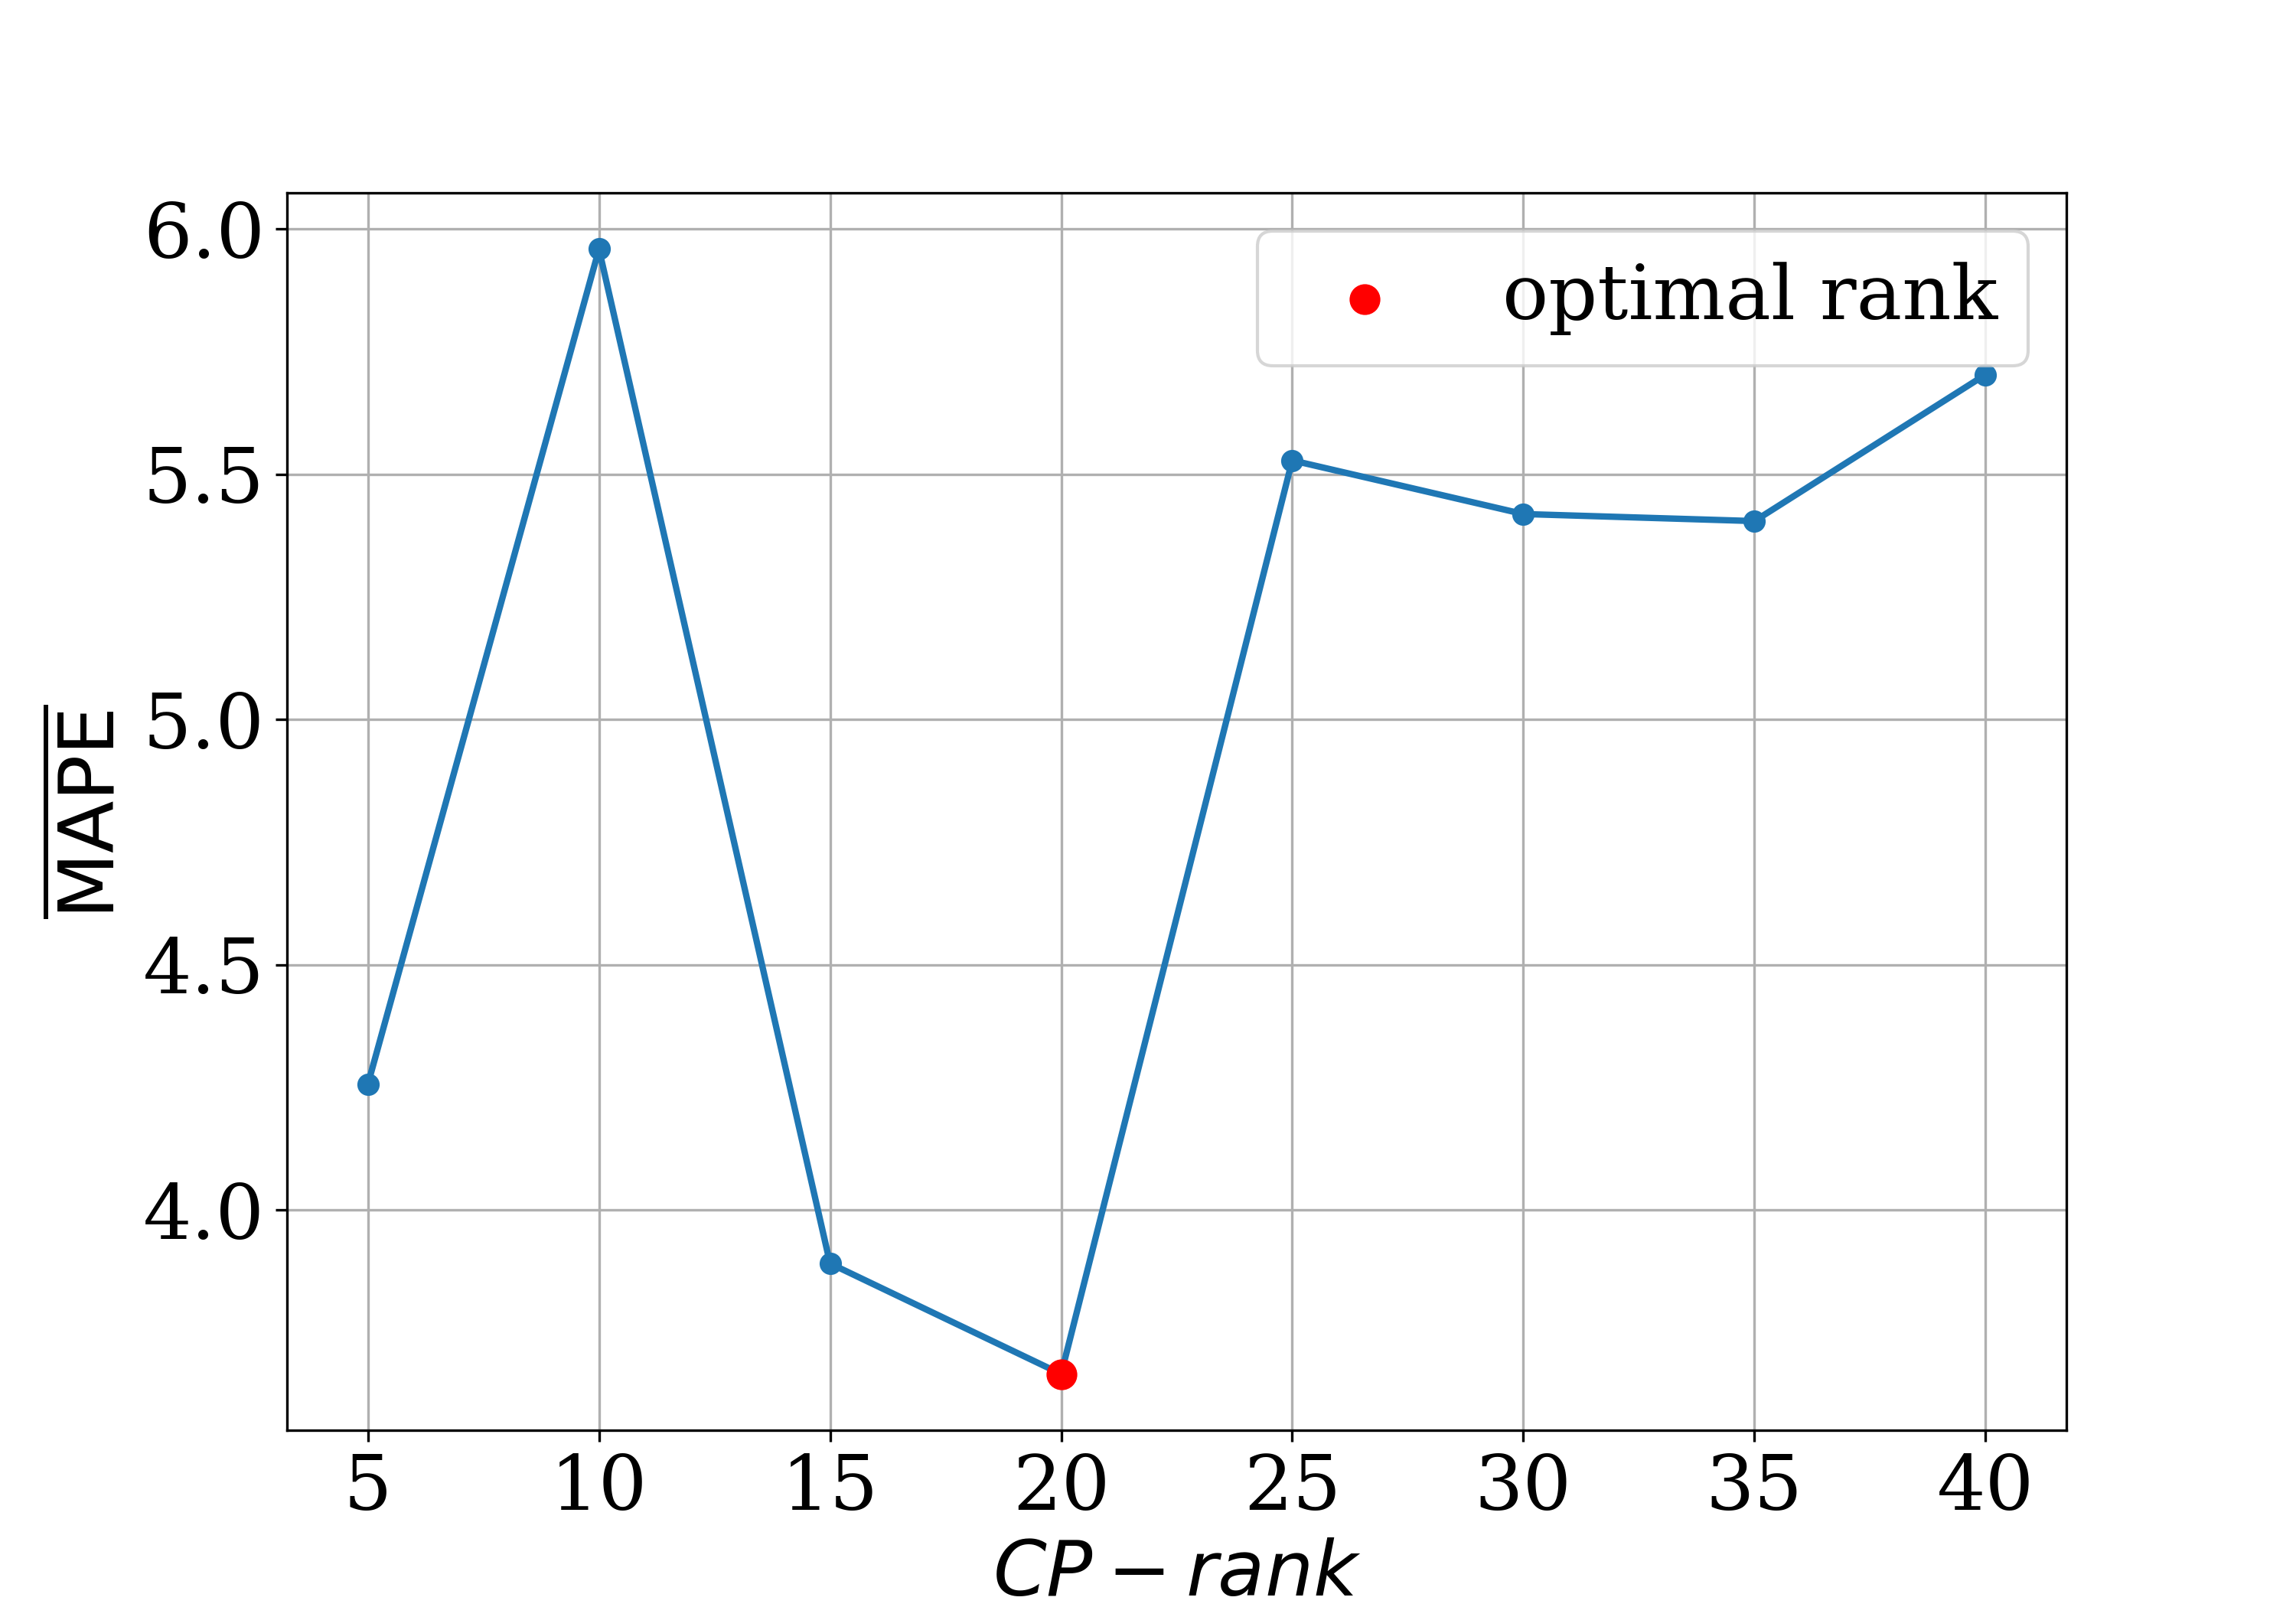
\includegraphics[width=0.48\textwidth, keepaspectratio]{pred_MAPE_rank_motion.png}
		\caption{$ \overline{\text{MSE}} $ and $ \overline{\text{MAPE}} $ metrics for the tSSA forecast depending on the CPD rank. An optimal point is marked with red. Inertial unit data.}\label{fig:mse_mape_motion}
	\end{figure}
	
	\begin{figure}[!htbp]
		\centering
		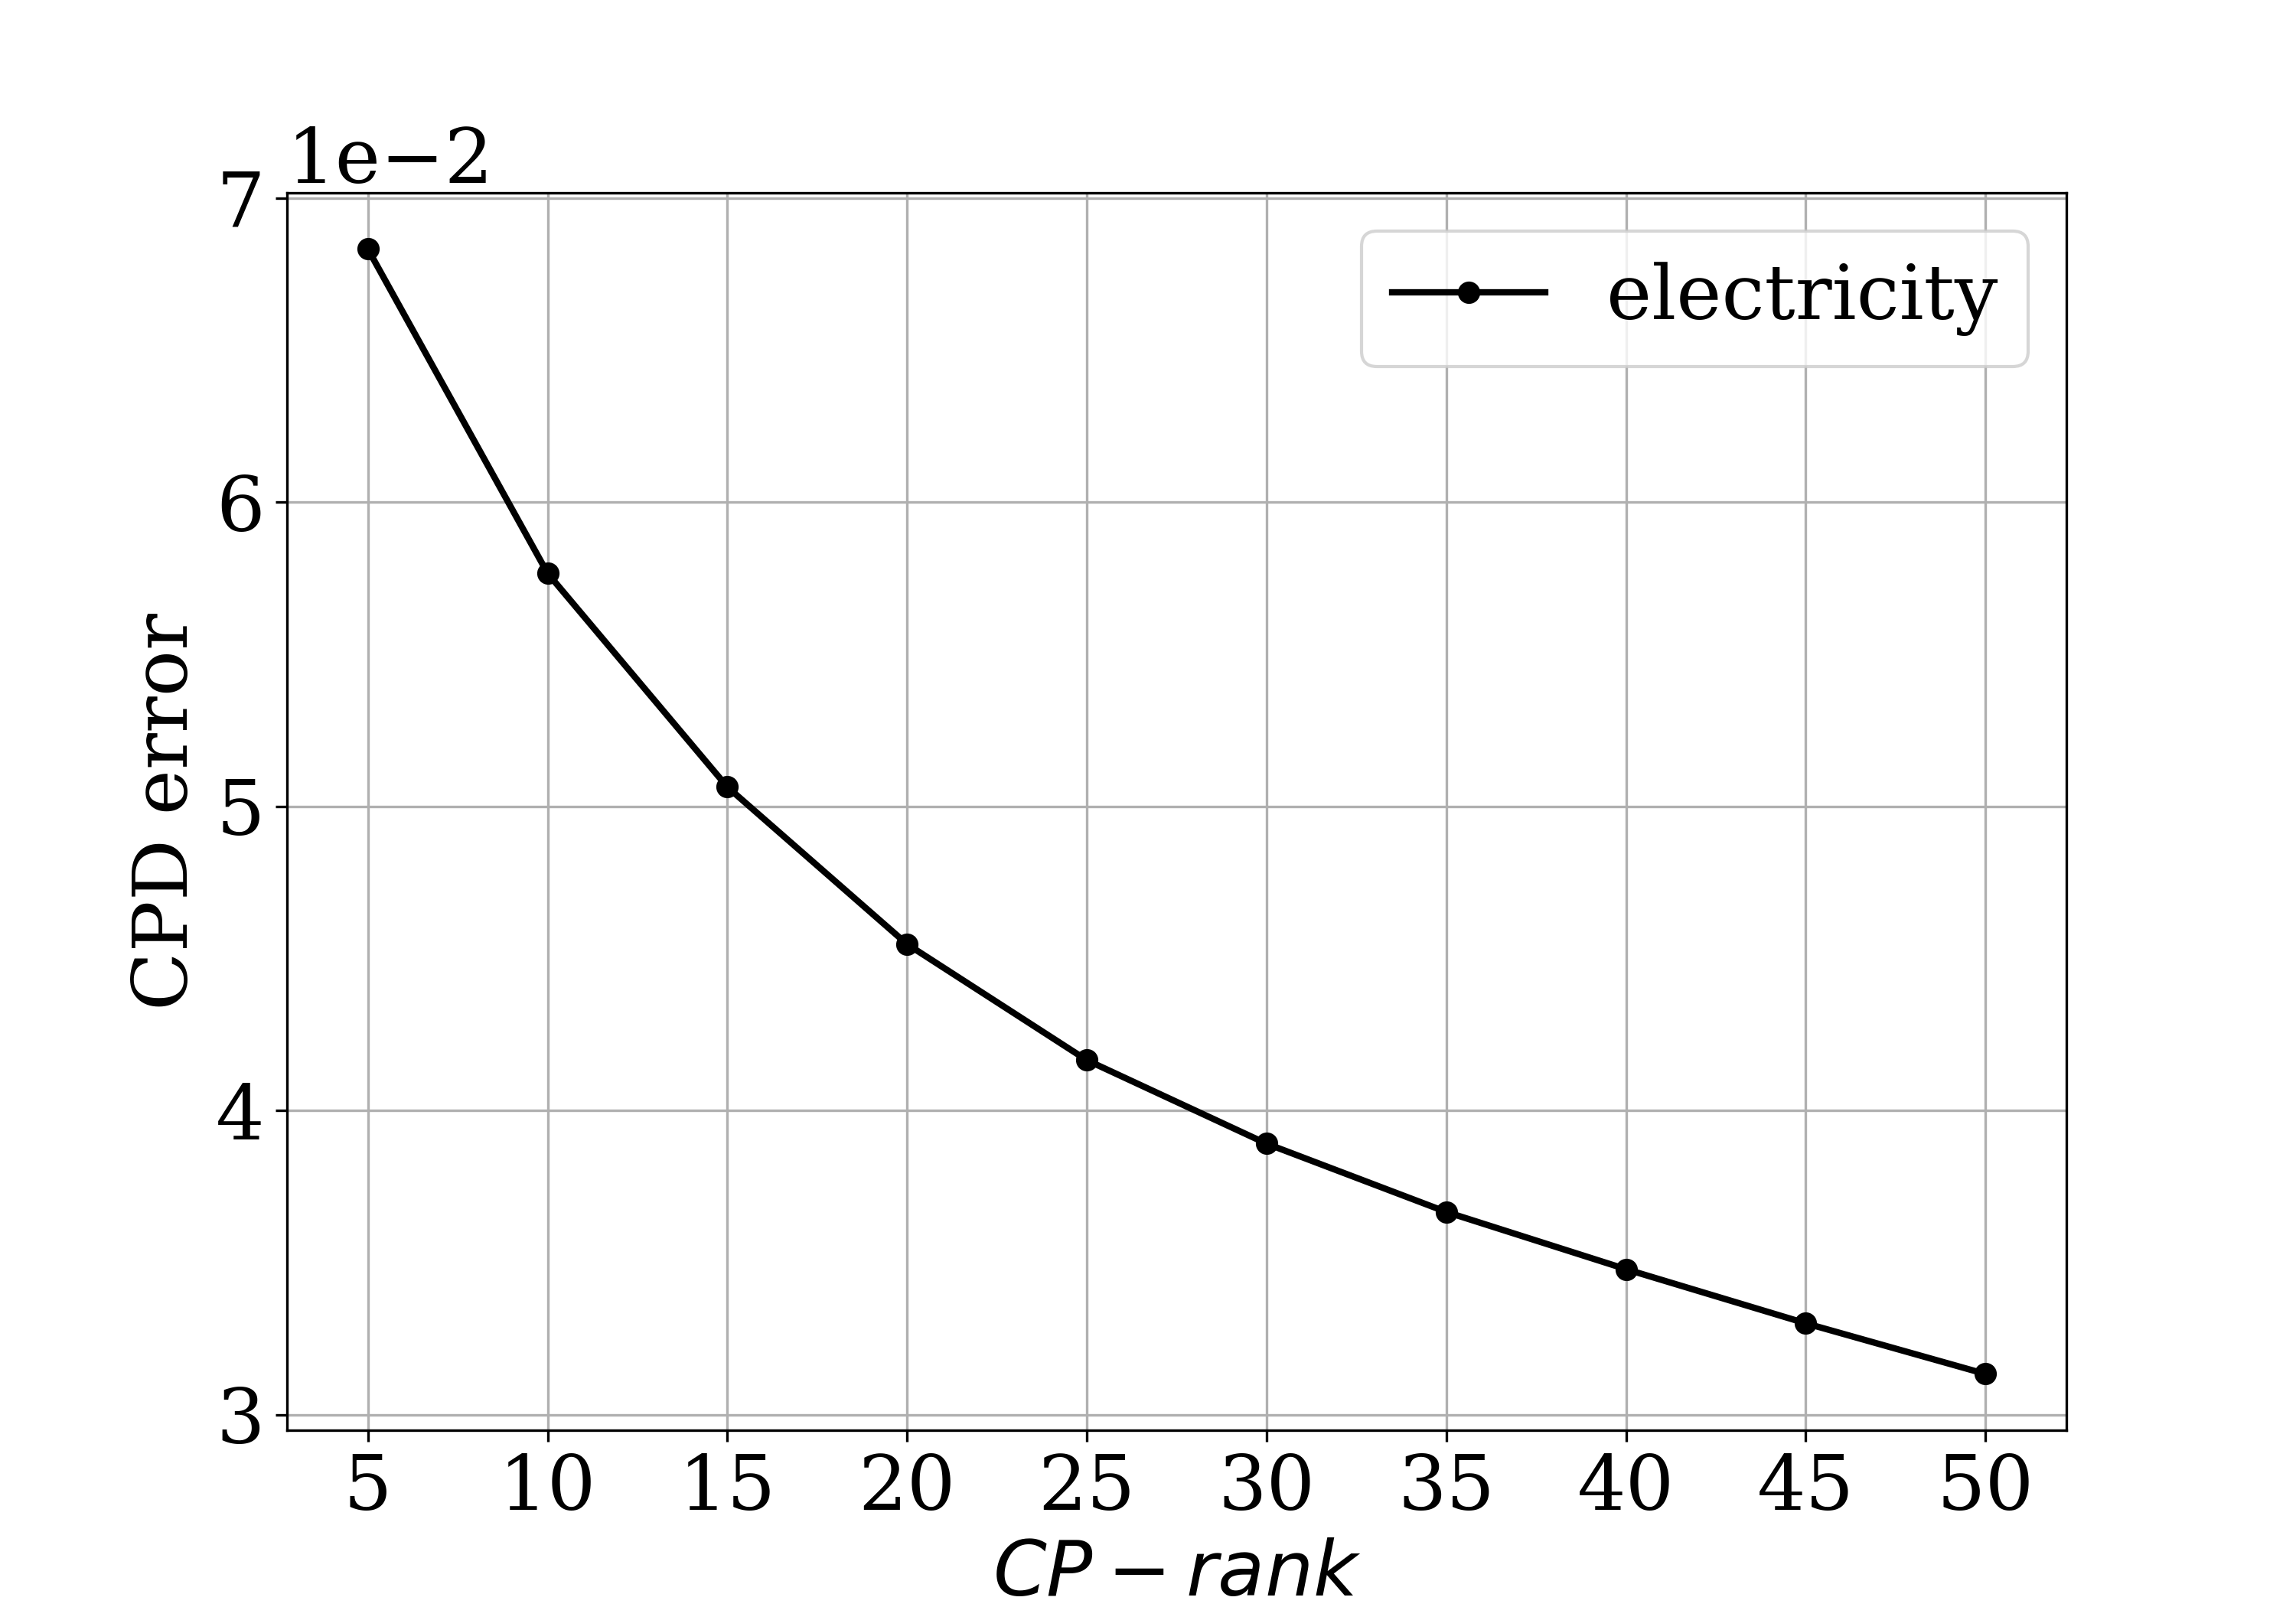
\includegraphics[width=0.48\textwidth, keepaspectratio]{CPD_error_elec.png}
		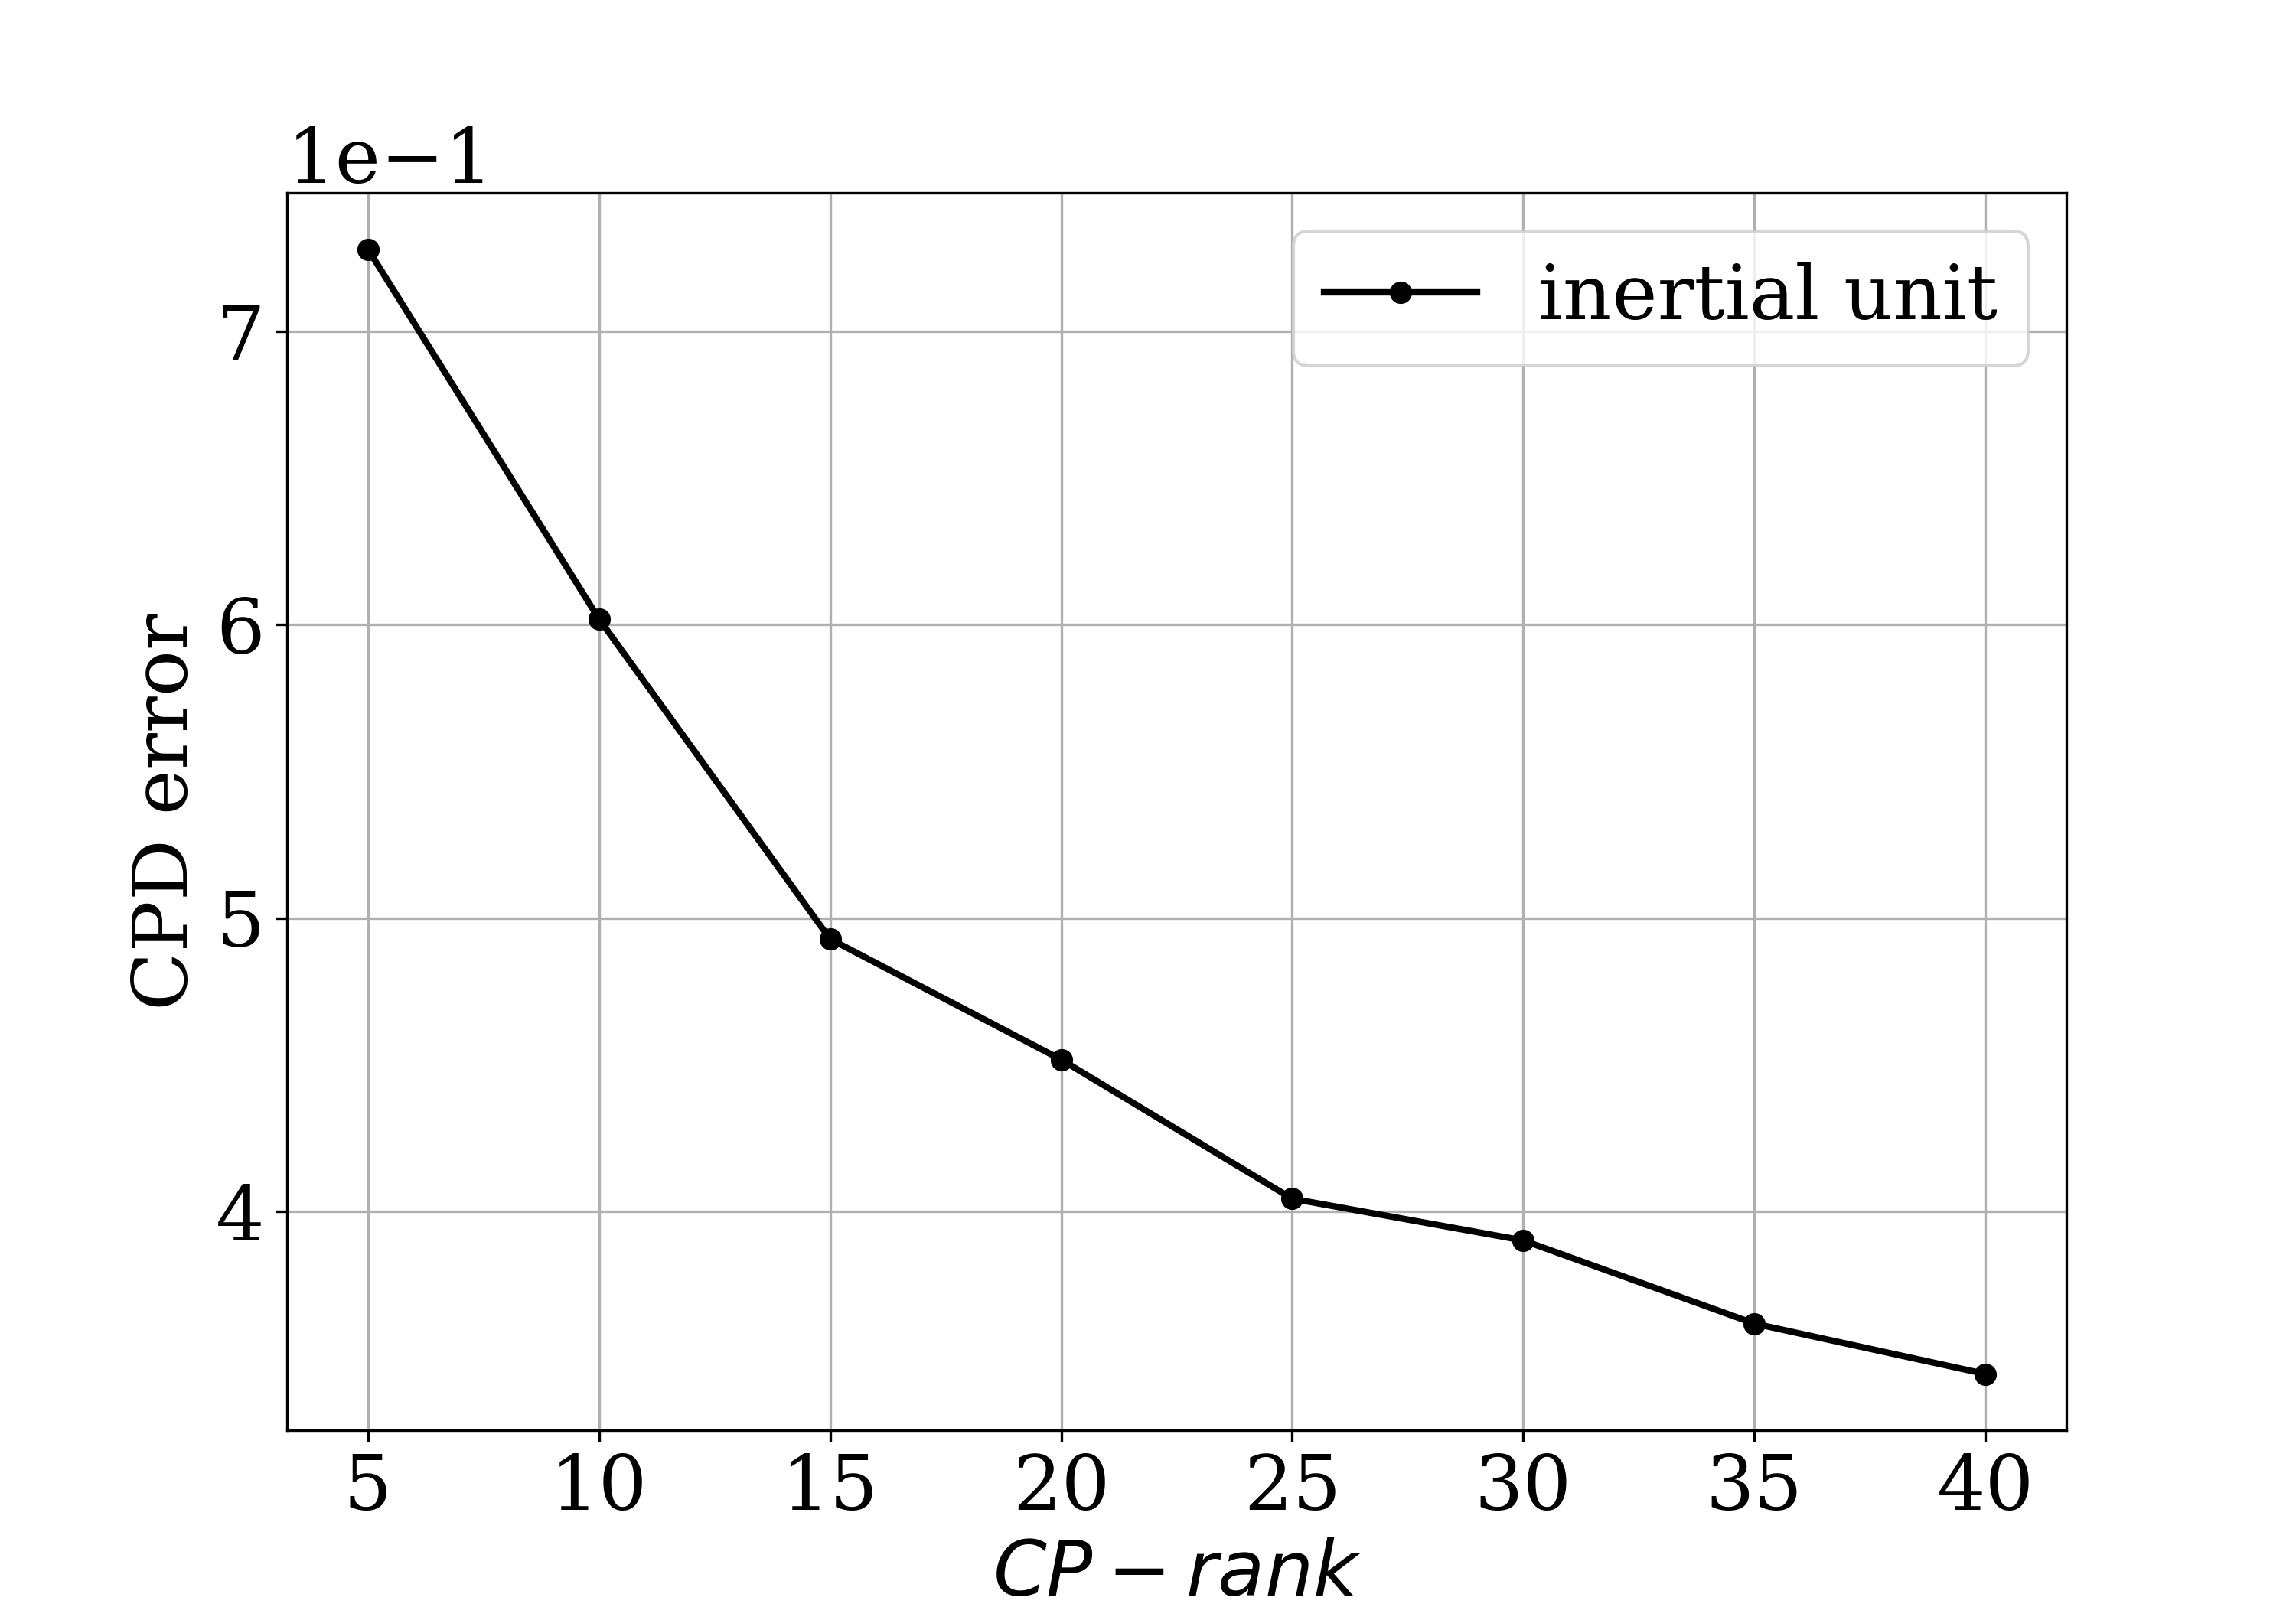
\includegraphics[width=0.48\textwidth, keepaspectratio]{CPD_error_motion.png}
		\caption{Relative CPD computation error depending on the CPD rank. The left is for the electricity data, the right is for the inertial unit data.}\label{fig:cpd_errors}
	\end{figure}
	
	Tab. \ref{tab:pred_res_electr} and \ref{tab:pred_res_motion} contain the MAPE and MSE metrics for all models. Our method showed the best results in most cases. Close values were obtained with the mSSA. The VAR model appeared unstable for the test samples. The RNN learned only the constant function from the electricity samples. But with the greater $ L $ for the inertial unit samples, the RNN performed better.
	
	\def\arraystretch{1.2}
	\begin{table}[h]
		\centering
		\caption{Forecast quality of the models on the electricity data}\label{tab:pred_res_electr}
		\begin{tabular}{|l|c|c|c|c|}
			\hline
			\diagbox{Metric}{Method} & \textit{tSSA}  & \textit{mSSA} & \textit{VAR} & \textit{RNN} \\ \hline
			$ \overline{\text{MSE}}_{\text{Producution}} $, $10^6$ & 1.24           & 1.51          & 7.81         & 2.70         \\ \hline
			$ \overline{\text{MSE}}_{\text{Price}} $, $10^3$      & 0.88           & 1.03          & 4.85         & 30.0         \\ \hline
			$ \overline{\text{MSE}} $, $10^6$             & \textbf{0.62}  & 0.75          & 3.91         & 135.00       \\ \hline
			$ \overline{\text{MAPE}}_{\text{Producution}} $        & 0.054          & 0.060         & 0.137        & 0.999        \\ \hline
			$ \overline{\text{MAPE}}_{\text{Price}} $             & 0.164          & 0.170         & 0.360        & 1.004        \\ \hline
			$ \overline{\text{MAPE}} $                    & \textbf{0.109} & 0.115         & 0.249        & 1.002        \\ \hline
		\end{tabular}
	\end{table}
	
	\def\arraystretch{1.2}
	\begin{table}[h]
		\centering
		\caption{Forecast quality of the models on the inertial unit data}\label{tab:pred_res_motion}
		\begin{tabular}{|l|c|c|c|c|}
			\hline
			\diagbox{Metric}{Method} & \textit{tSSA}                & \textit{mSSA} & \textit{VAR} & \textit{RNN} \\ \hline
			$ \overline{\text{MSE}}_{\text{Accel}} $  & 7.351          & 6.980 & 8.108  & 6.604          \\ \hline
			$ \overline{\text{MSE}}_{\text{Gyro}} $   & 0.610          & 0.636 & 0.631  & 0.639          \\ \hline
			$ \overline{\text{MSE}} $         & 3.981          & 3.808 & 4.370  & \textbf{3.622} \\ \hline
			$ \overline{\text{MAPE}}_{\text{Accel}} $ & 3.558          & 3.516 & 3.370  & 1.747          \\ \hline
			$ \overline{\text{MAPE}}_{\text{Gyro}} $  & 3.773          & 3.943 & 10.427 & 5.641          \\ \hline
			$ \overline{\text{MAPE}} $        & \textbf{3.666} & 3.730 & 6.899  & 3.694          \\ \hline
		\end{tabular}
	\end{table}
	
	\paragraph{The decomposition}
	
	Fig. \ref{fig:decomp_rhe_rank} illustrates the RHE reaches a minimum for the tensor rank $ = 20 $. As the rank goes greater, the RHE does not change or even increase. The forecast quality had the same pattern. Therefore, small tensor ranks deliver the best quality for the decomposition and forecast problems. At the same time, the rank is a value of the shared phase space dimension, see Th.~\ref{th:cpd_phase}. The delay vectors define phase trajectory and have dimension equals $ L $. Recall that $ L $ is set to $ 500 $ for the electricity samples and to $ 1000 $ for the inertial unit samples. As a result, the tSSA has significantly reduced dimensionality of the sample time series.
	
	\begin{figure}[h]
		\centering
		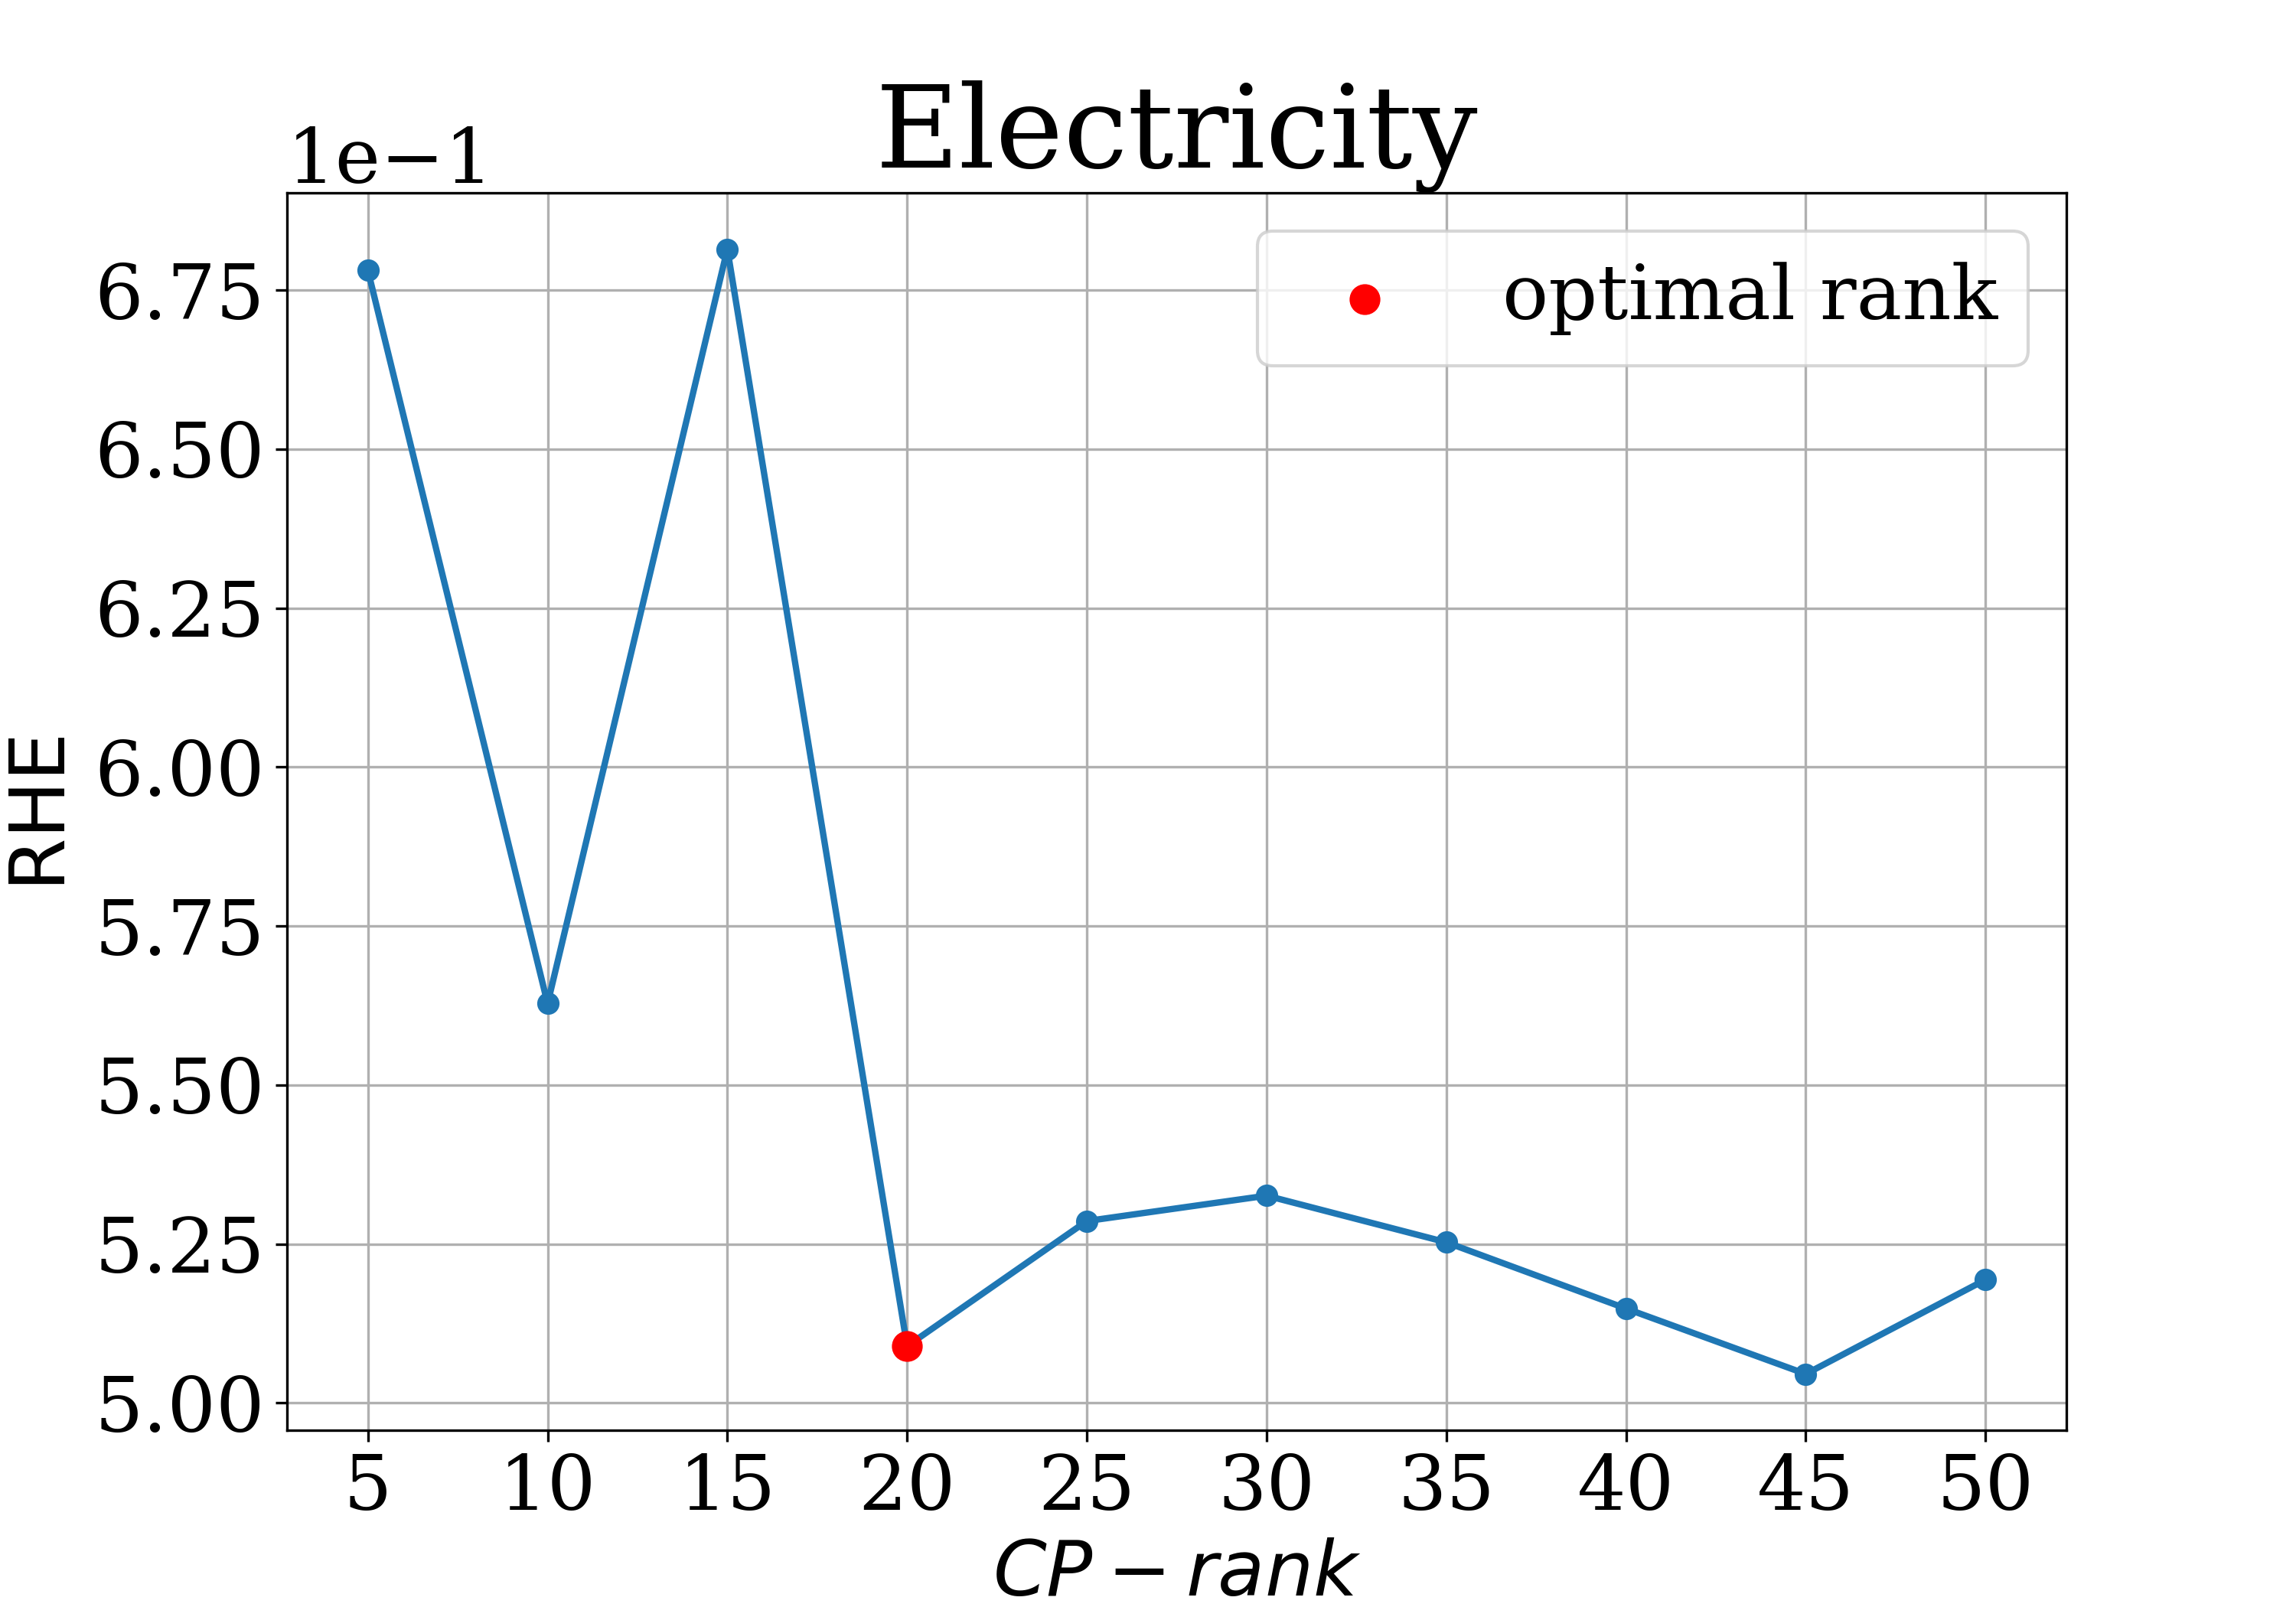
\includegraphics[width=0.48\textwidth, keepaspectratio]{RHE_mean_elec.png}
		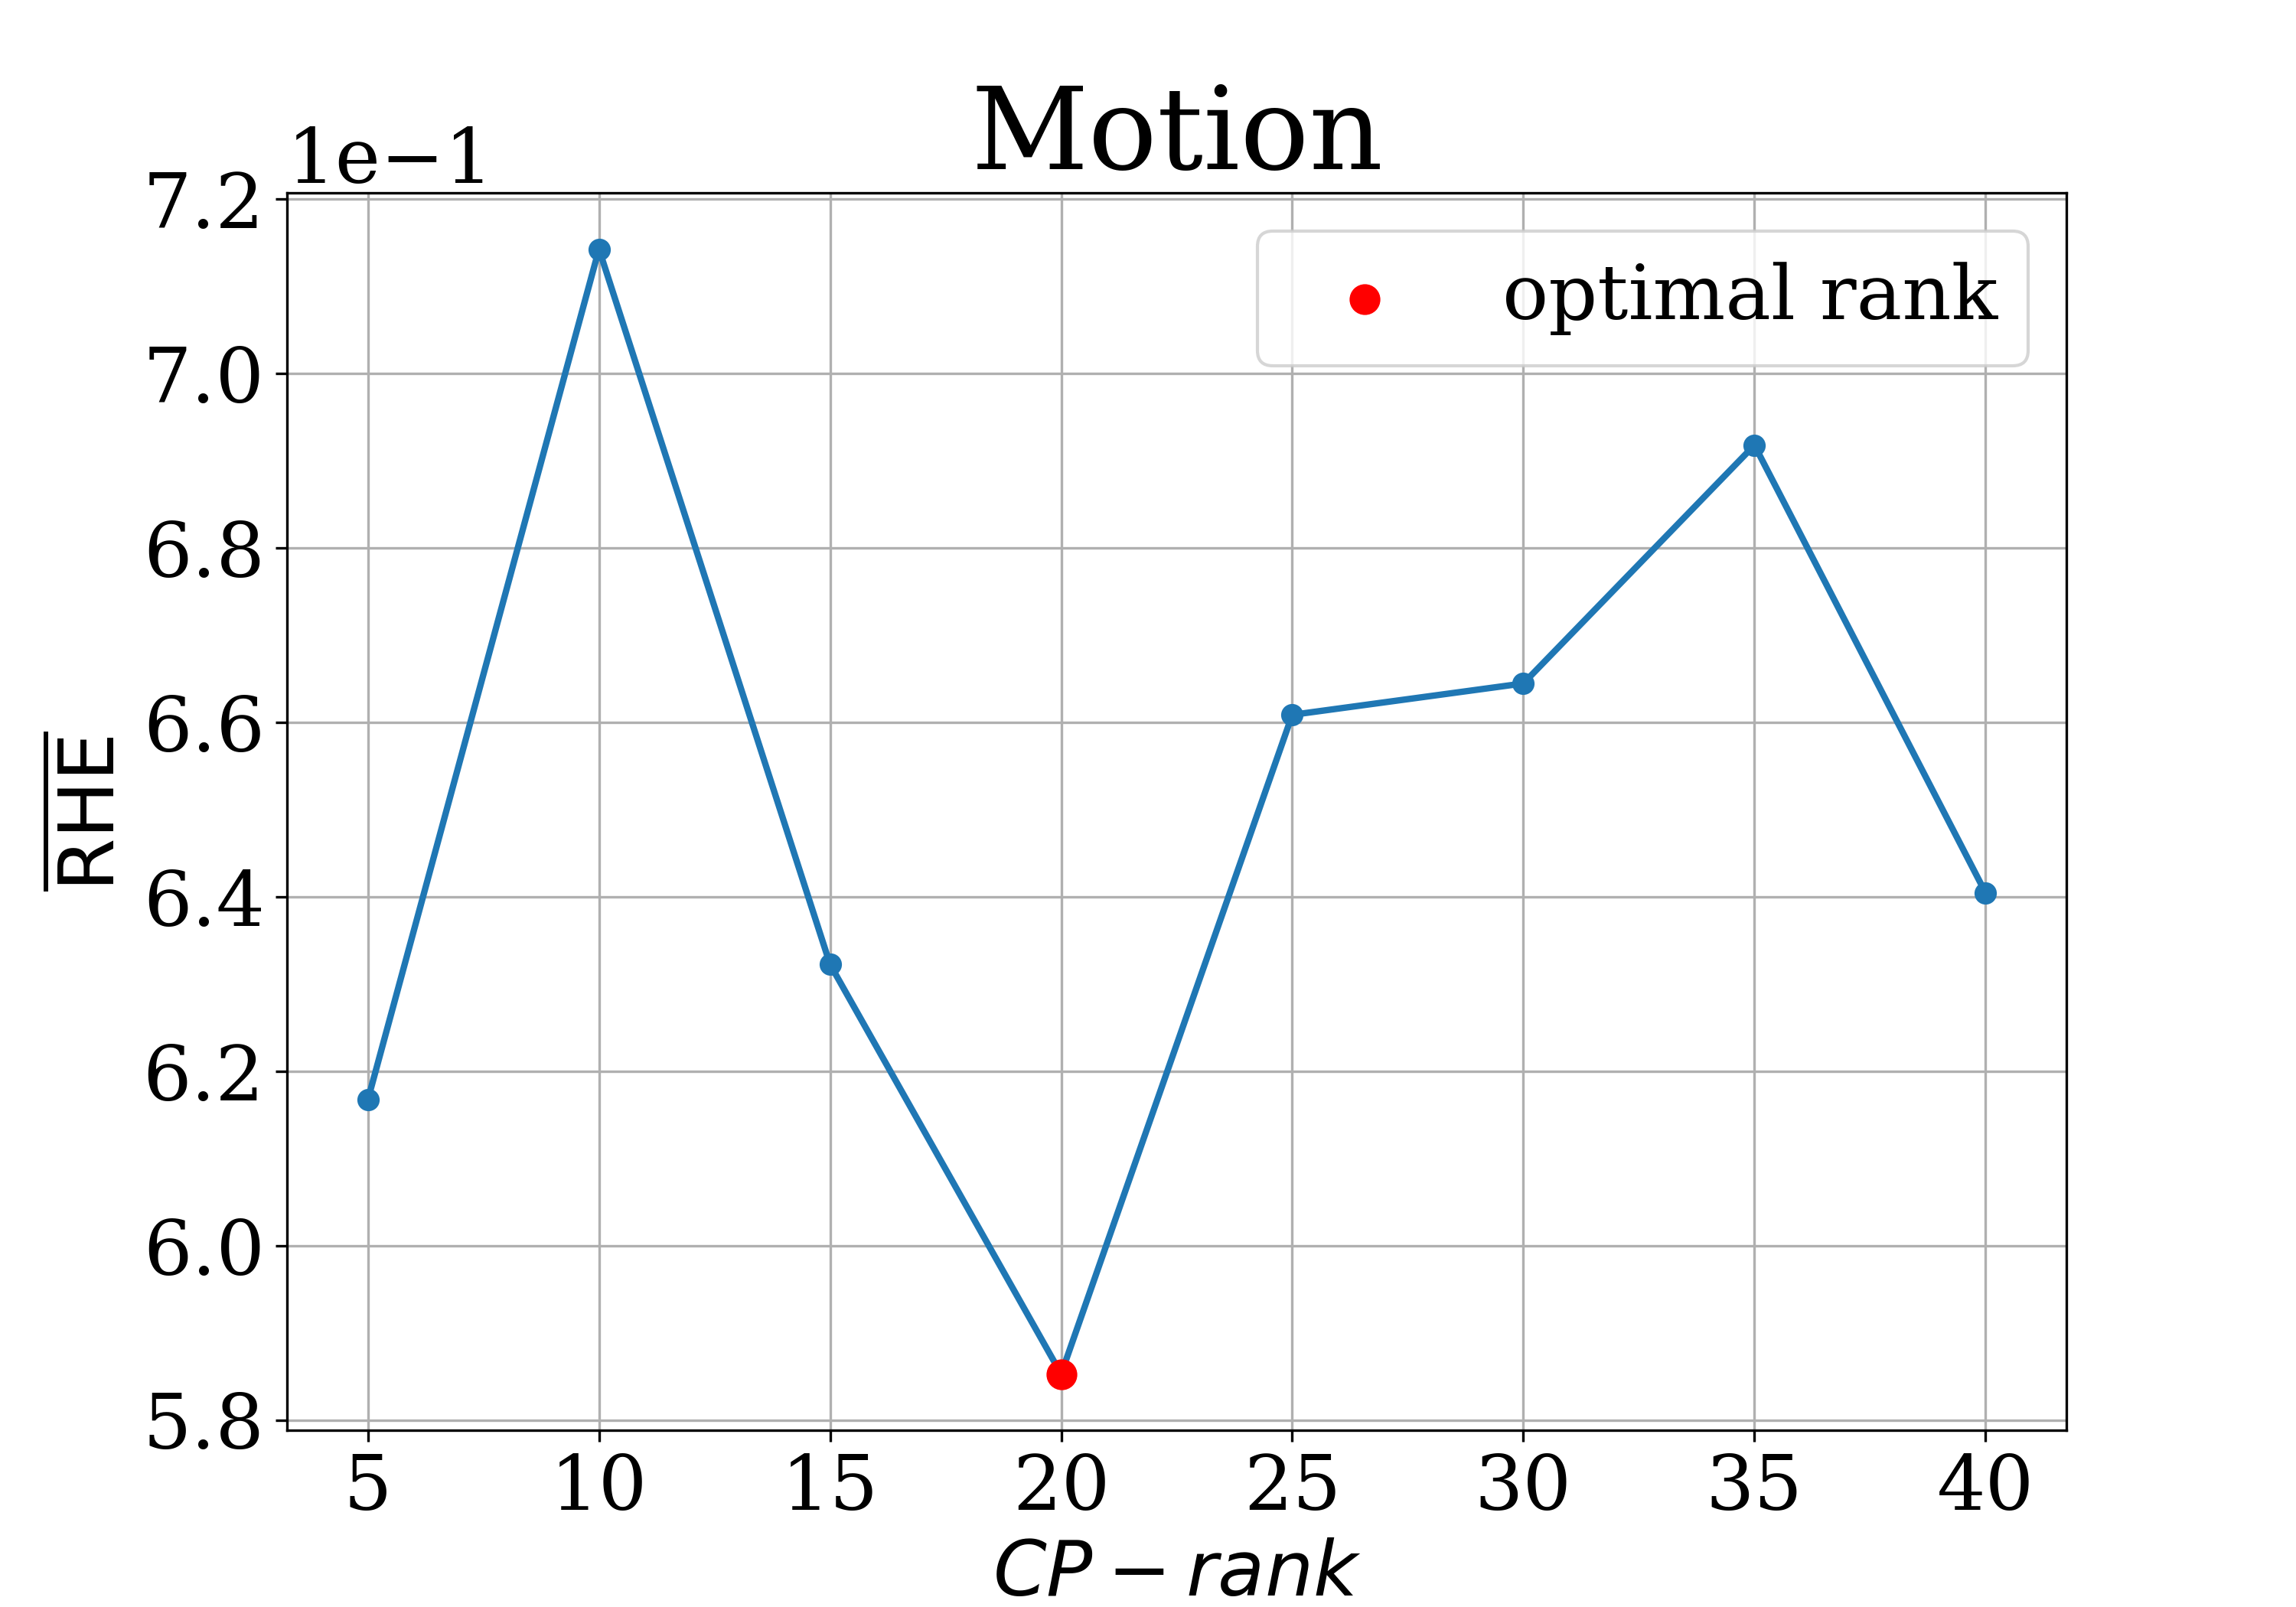
\includegraphics[width=0.48\textwidth, keepaspectratio]{RHE_mean_motion.png}
		\caption{The $ \overline{\text{RHE}} $ metrics depending on the CPD rank. The left is for the electricity data, the right is for the inertial unit data. An optimal point is marked with red}\label{fig:decomp_rhe_rank}
	\end{figure}
	
	Fig.~\ref{fig:electr_decomp_tssa} illustrates the decomposition on two components for the electricity consumption and price. The components are almost identical to the bias and scale factors. This is attributed to the \emph{shared} phase space between the time series. Fig.~\ref{fig:accel_decomp_tssa} shows two-component decomposition for the accelerometer and Fig~\ref{fig:gyro_decomp_tssa} shows the same for the gyroscope. The second components are identical to the rotation and scale. Moreover, all components here coincide with the phase trajectories. 
	
	\begin{figure}[h]
		\centering
		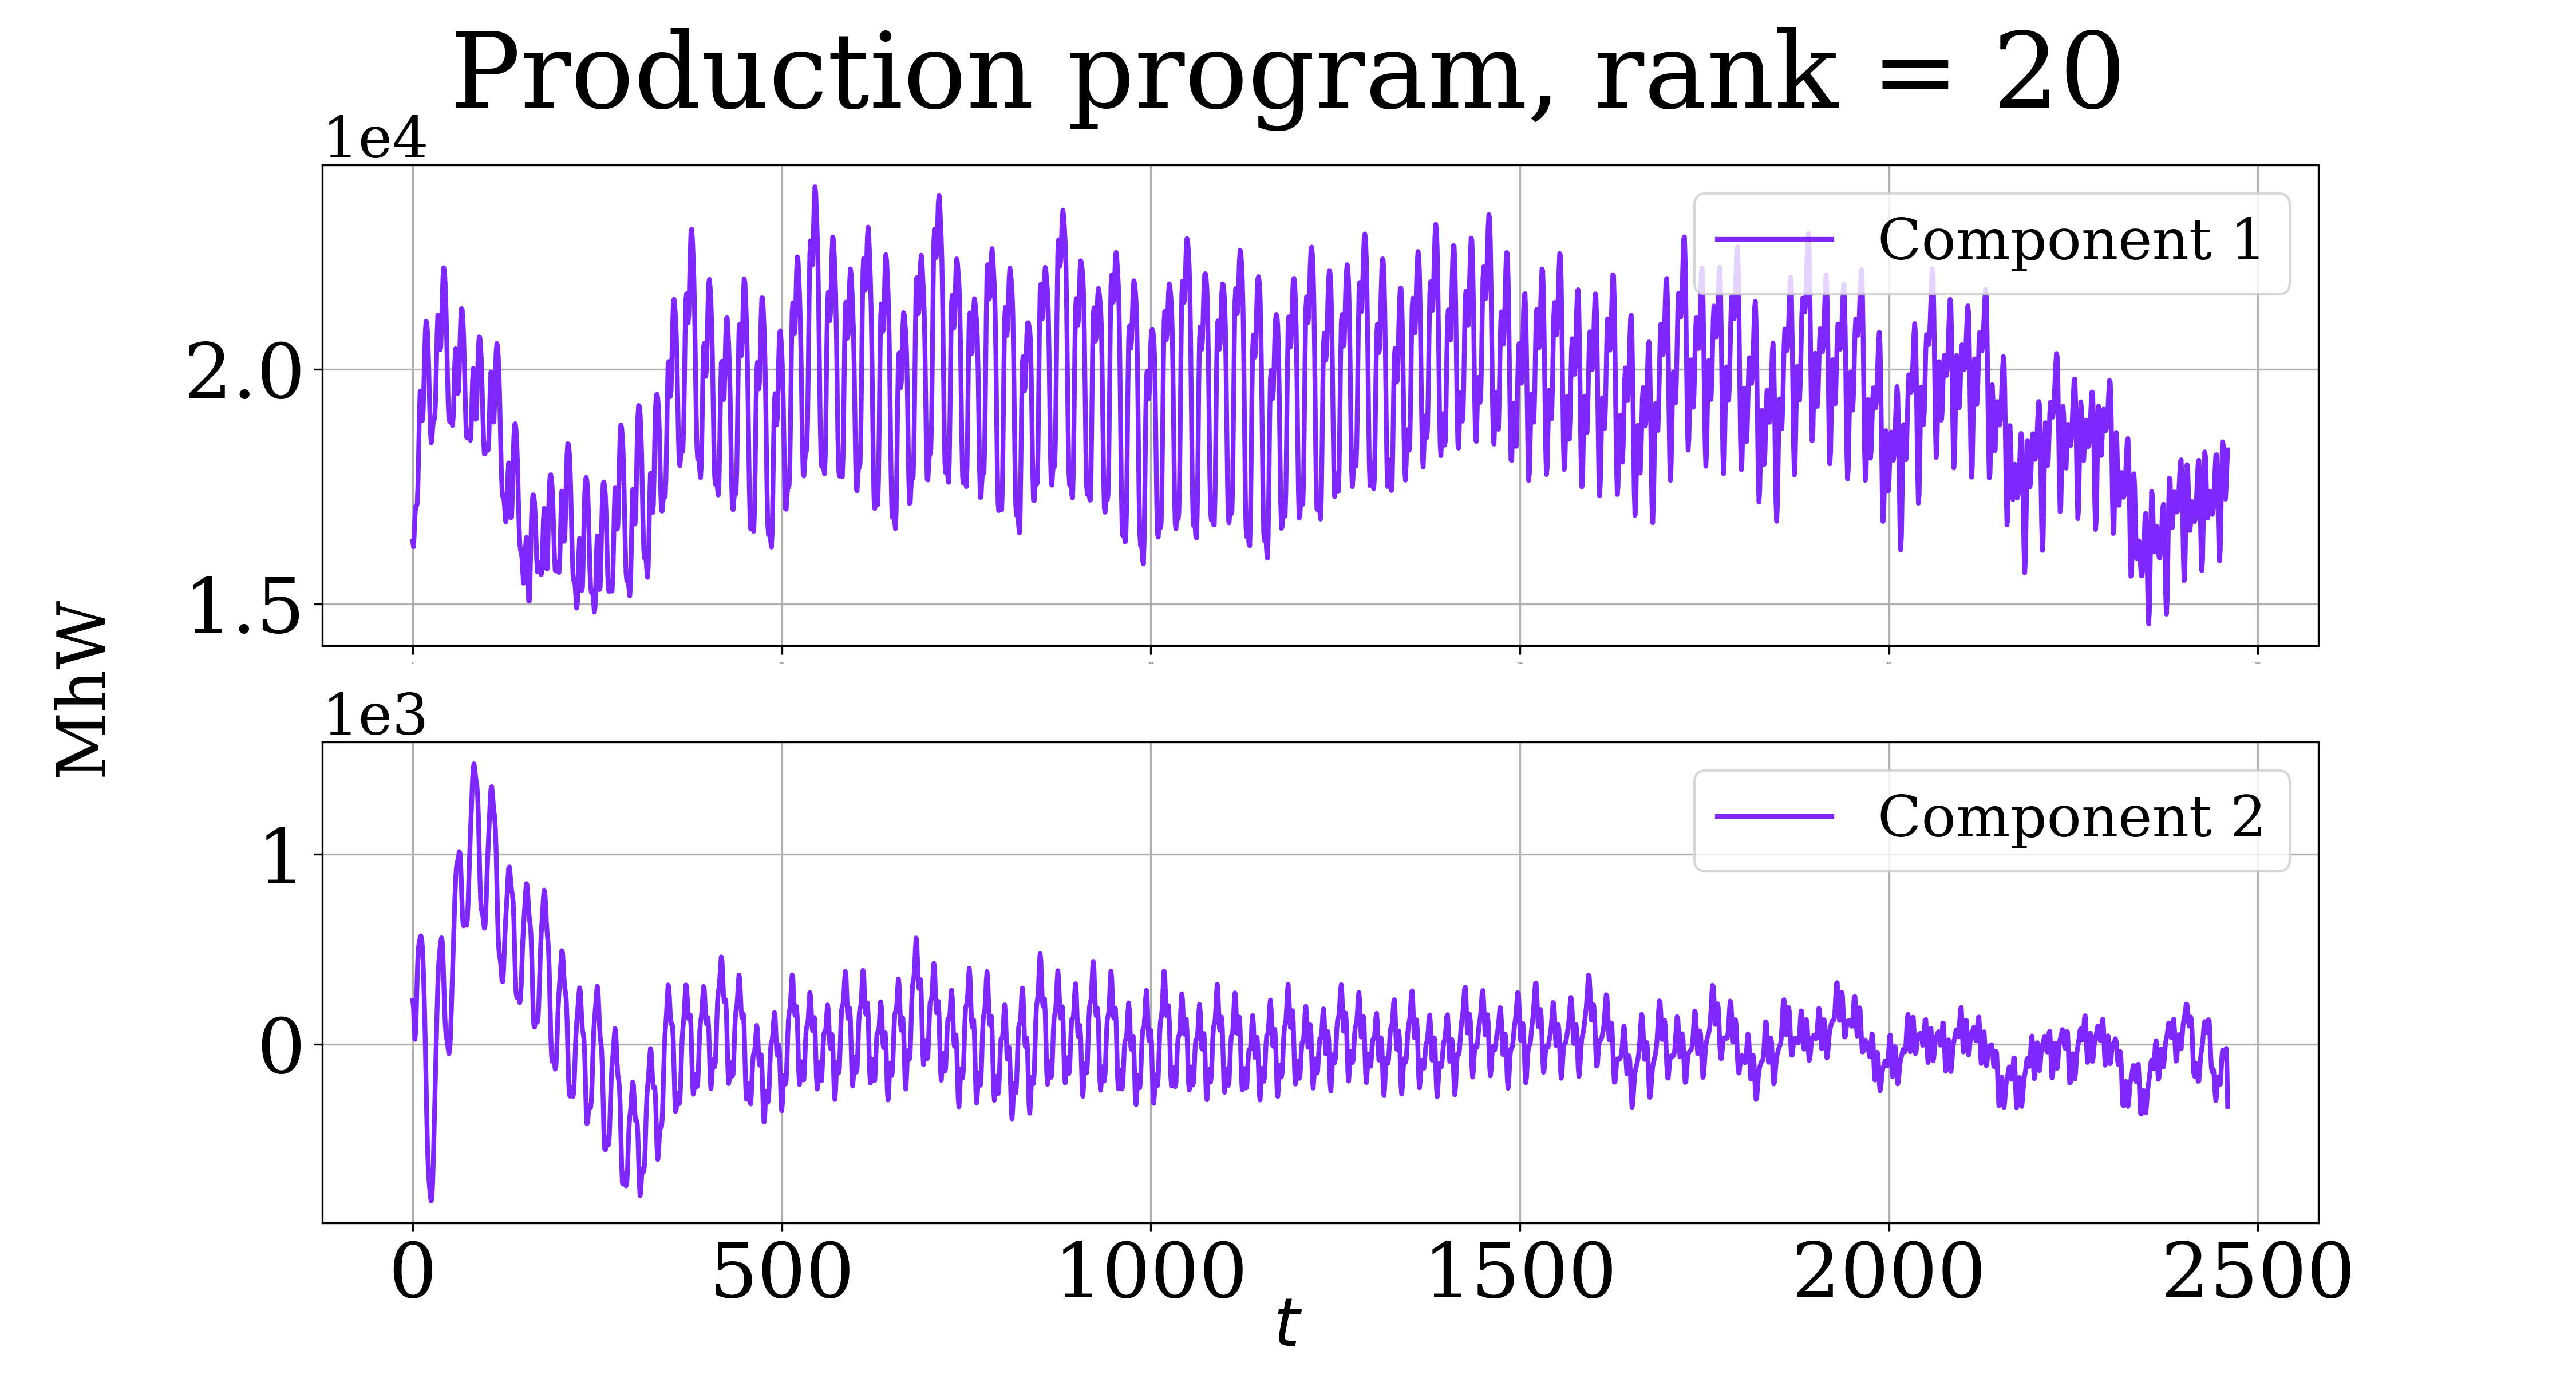
\includegraphics[width=0.48\textwidth, keepaspectratio]{Production program_decomp.png}
		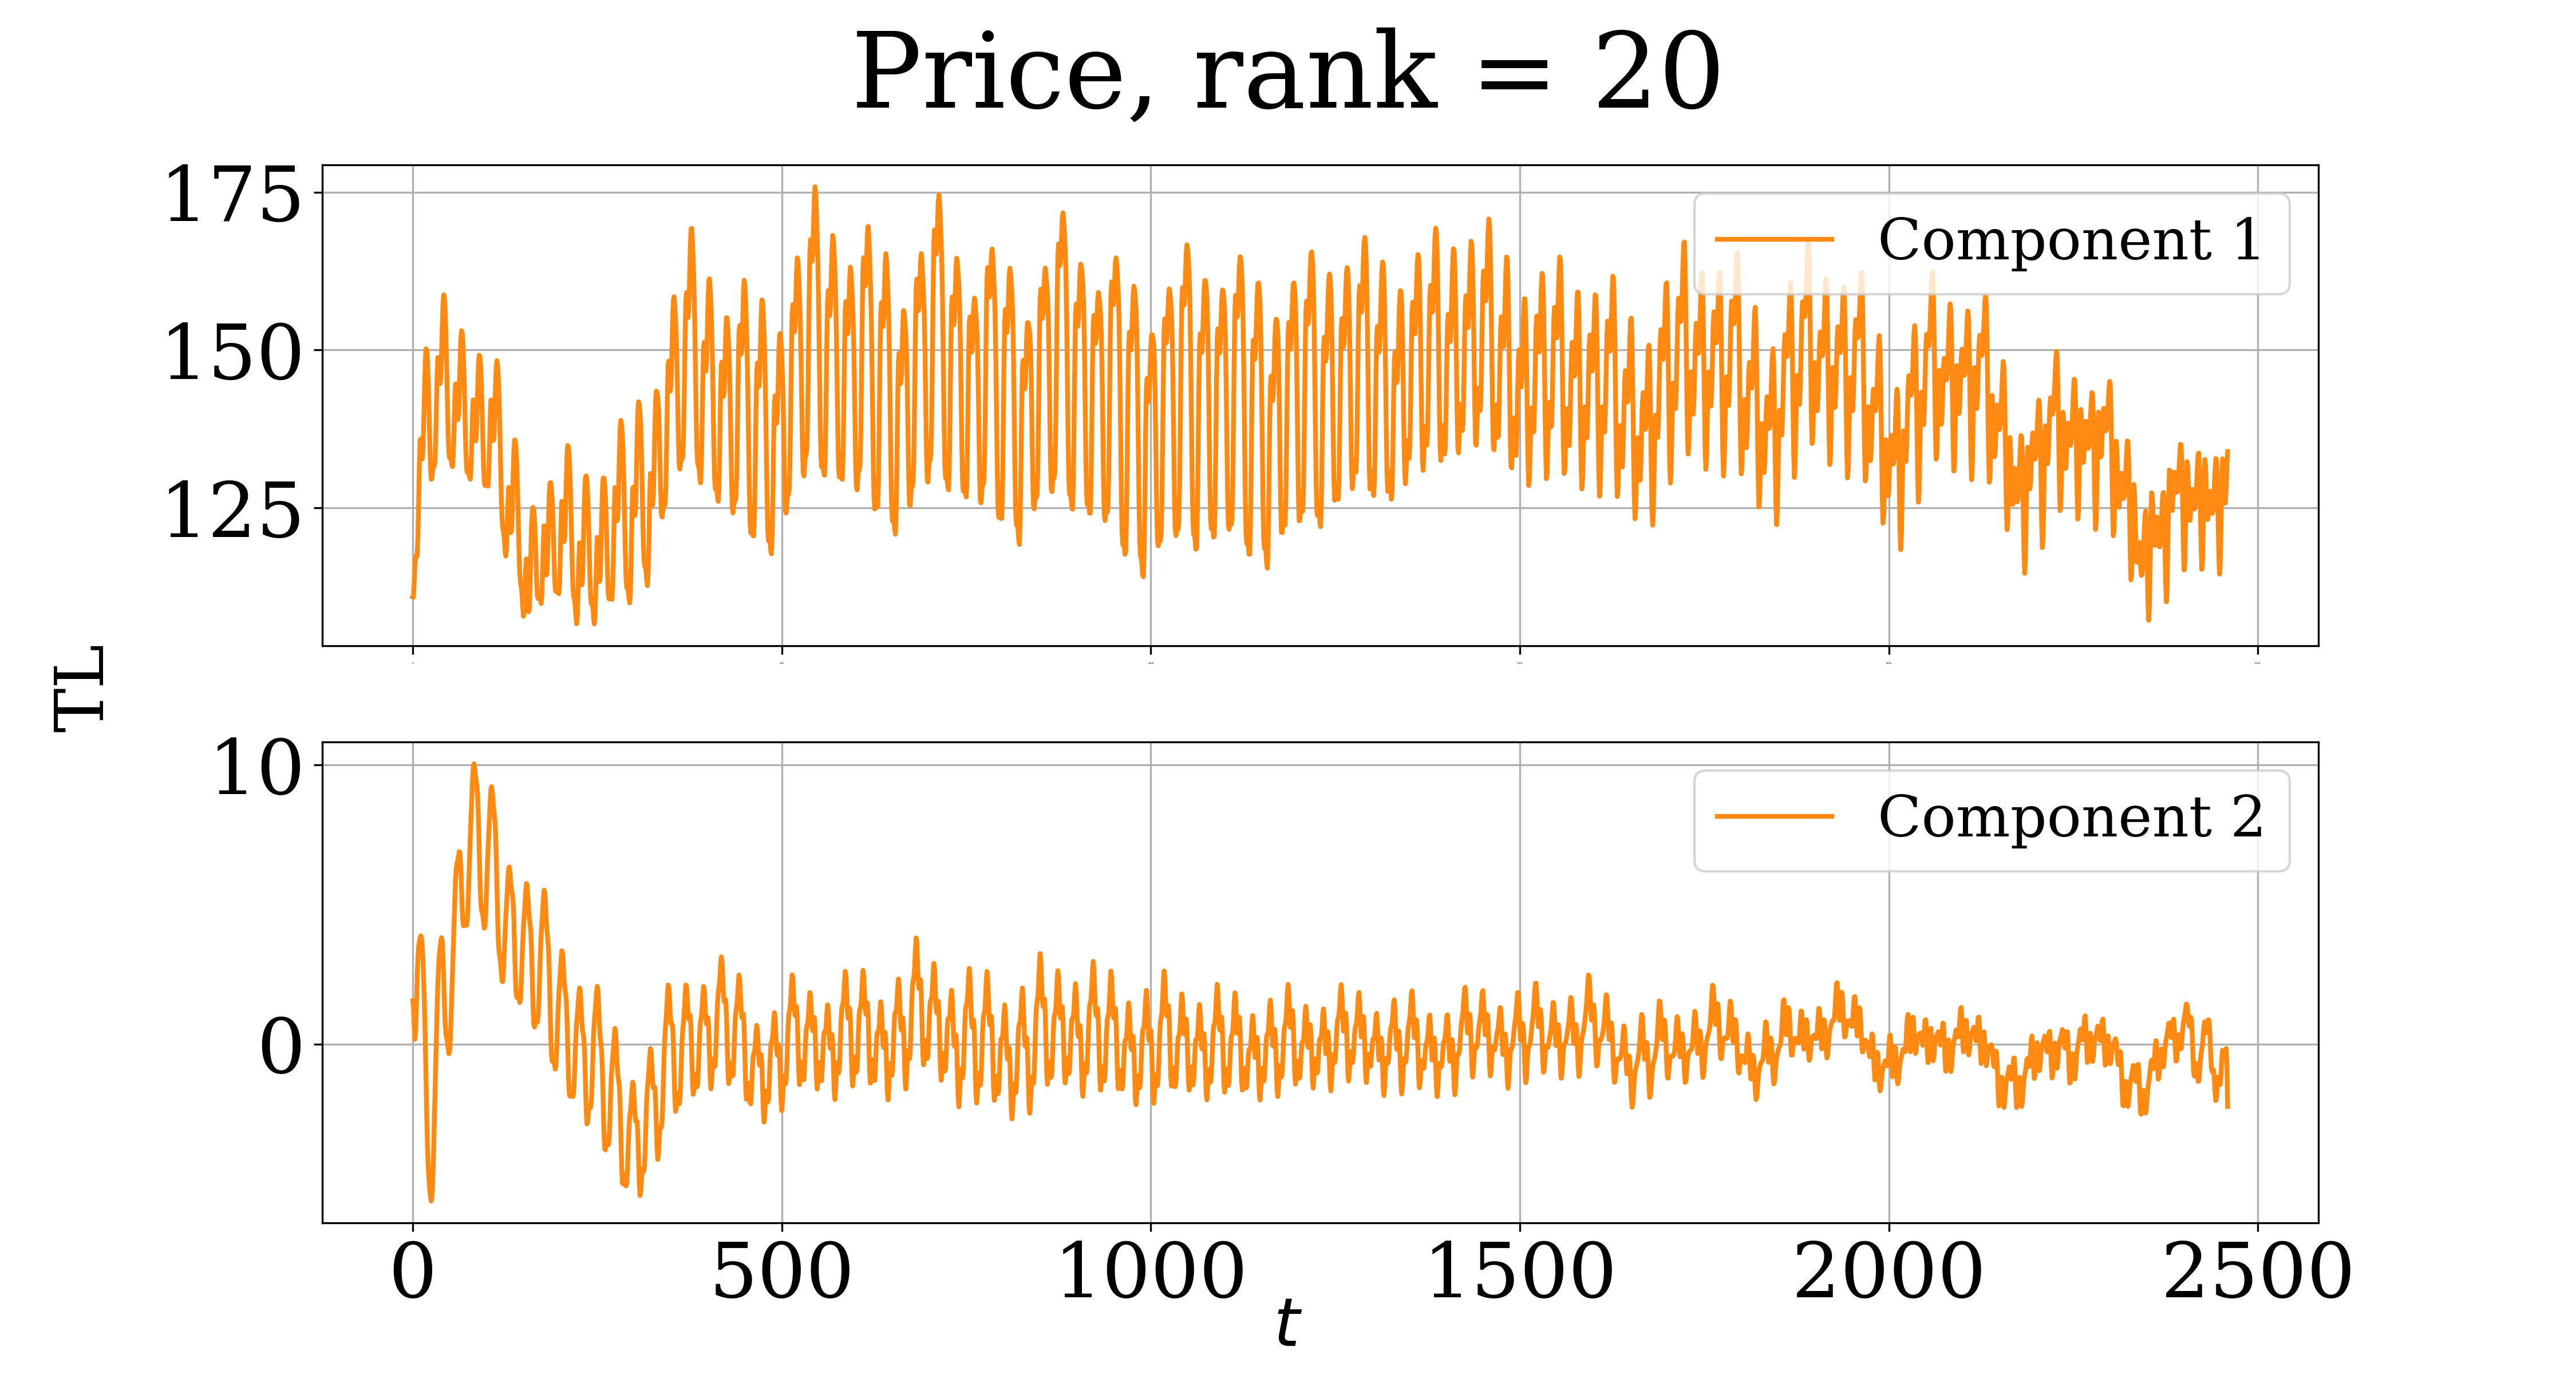
\includegraphics[width=0.48\textwidth, keepaspectratio]{Price_decomp.png}
		\caption{tSSA decomposition for the electricity data. CPD rank $ = 20 $}\label{fig:electr_decomp_tssa}
	\end{figure}
	
	\begin{figure}[h]
		\centering
		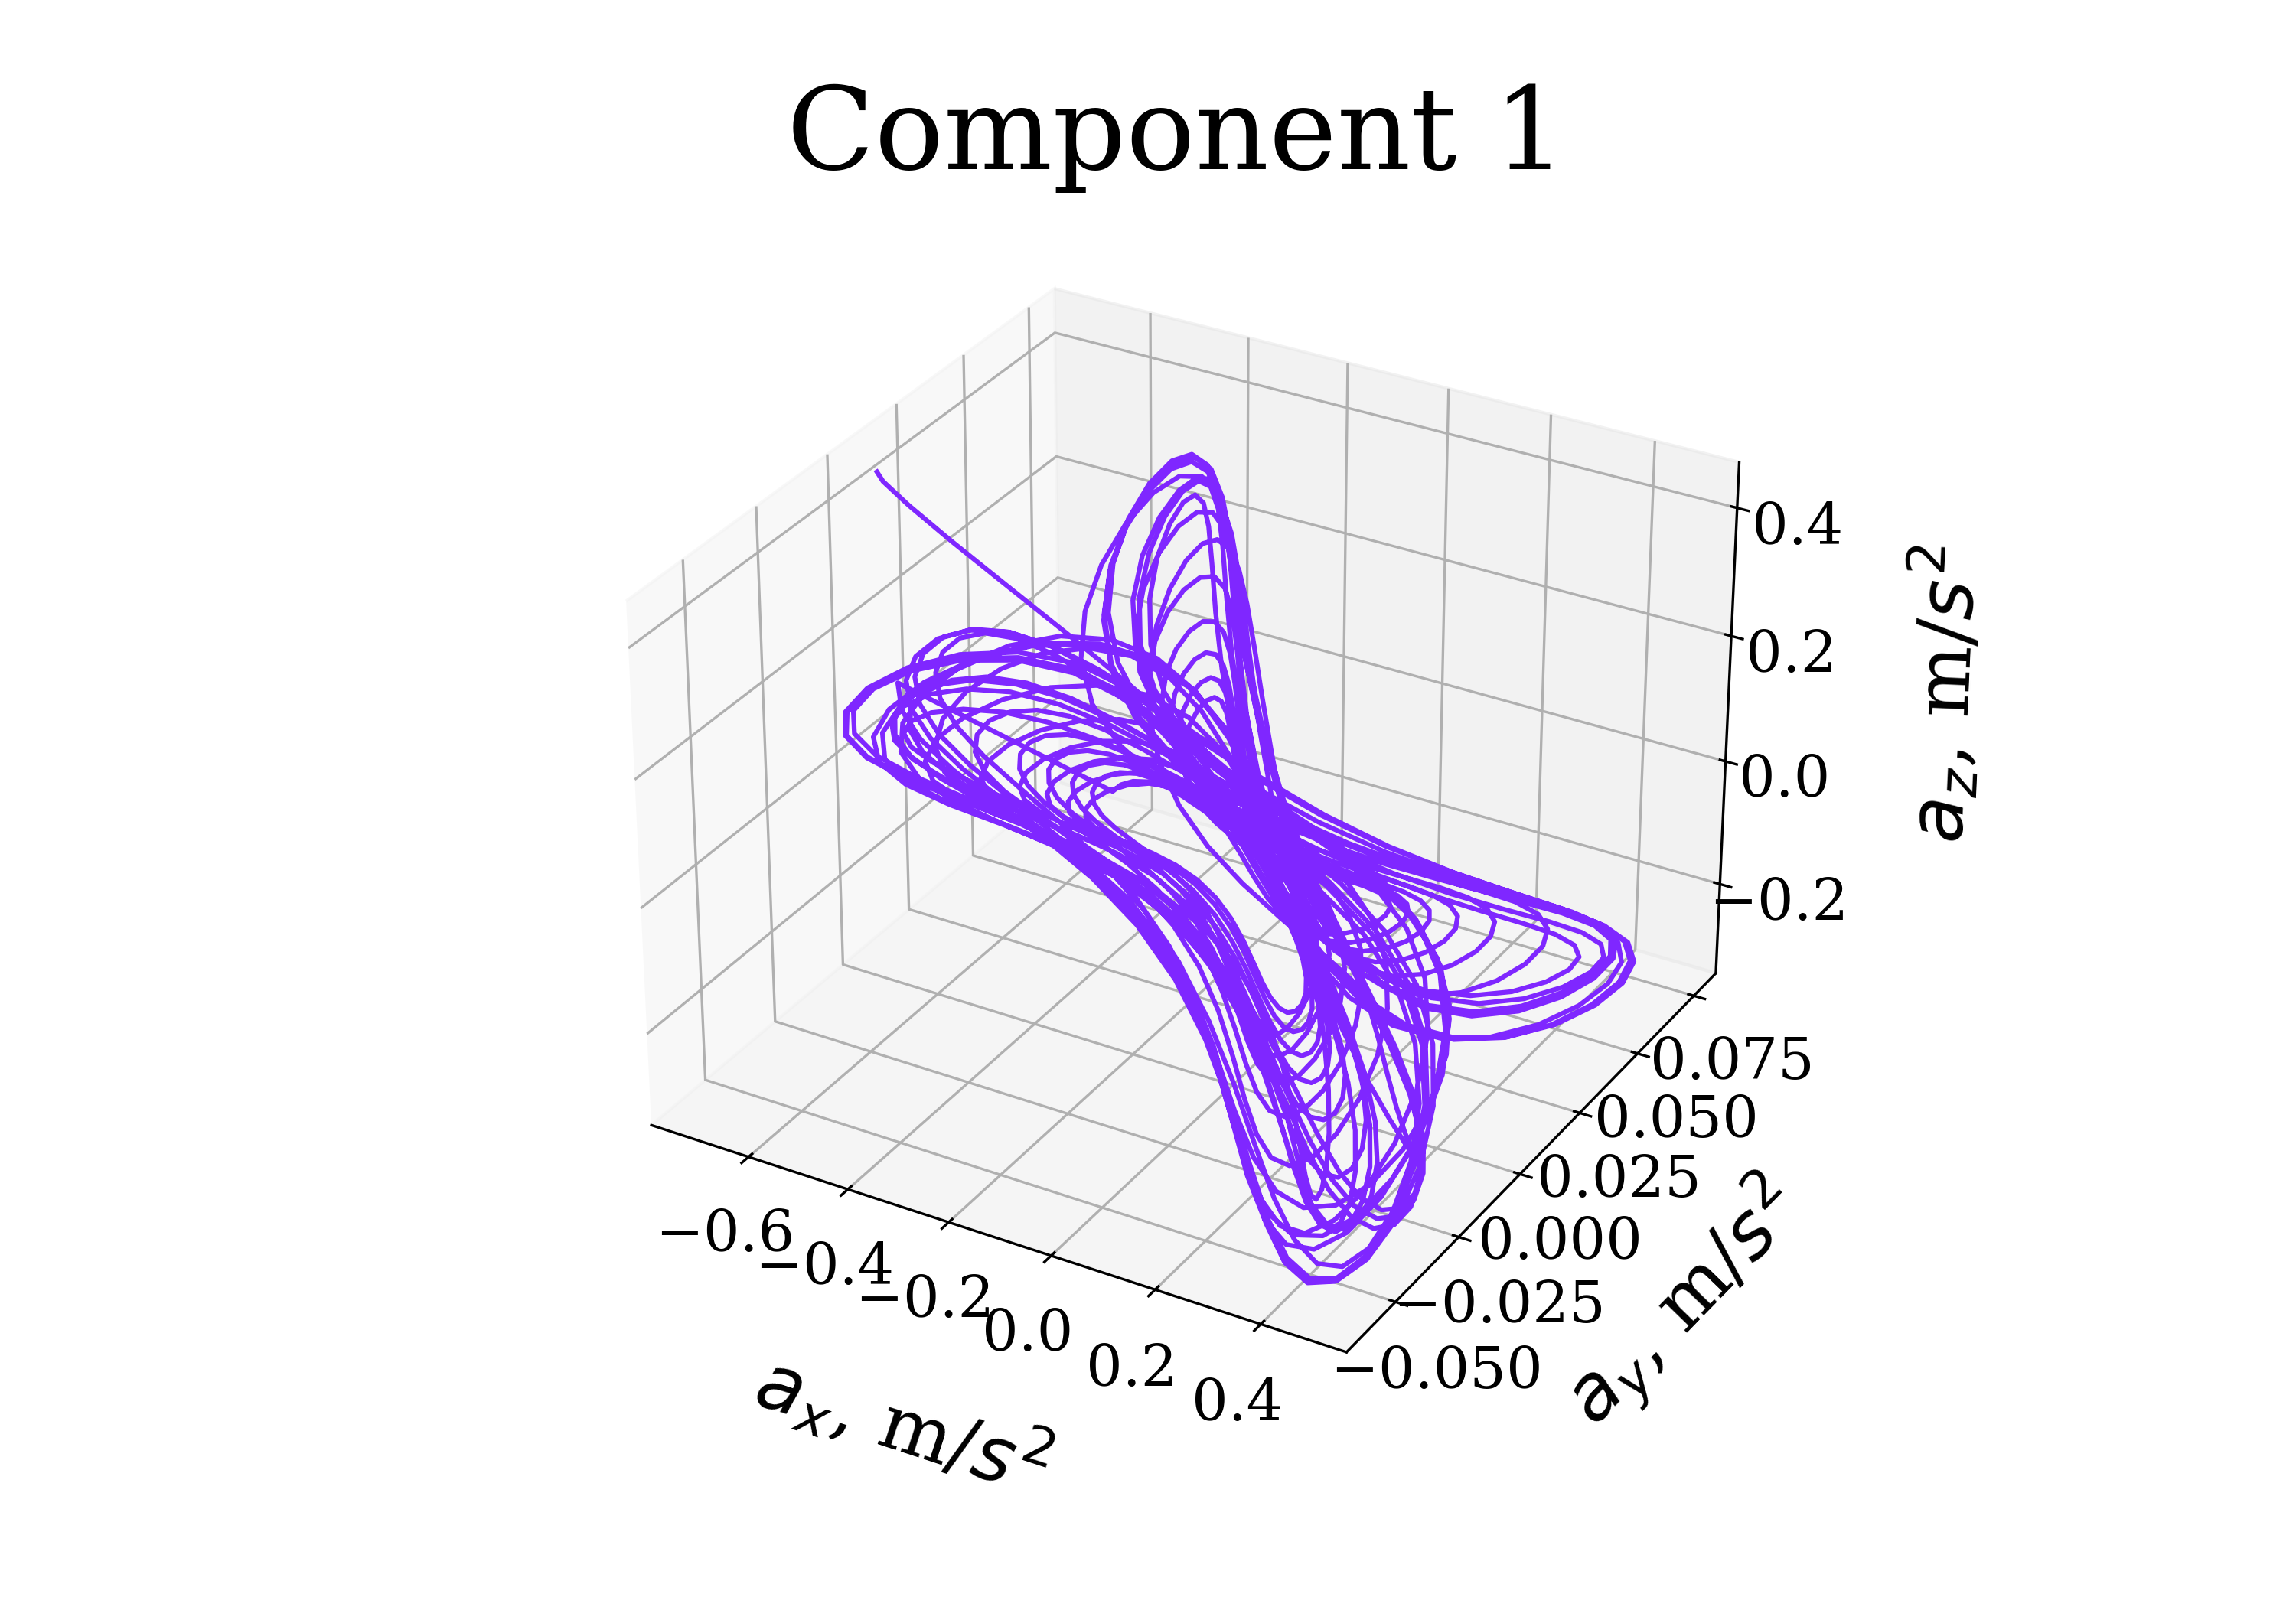
\includegraphics[width=0.48\textwidth, 	keepaspectratio]{acceler_1.png}
		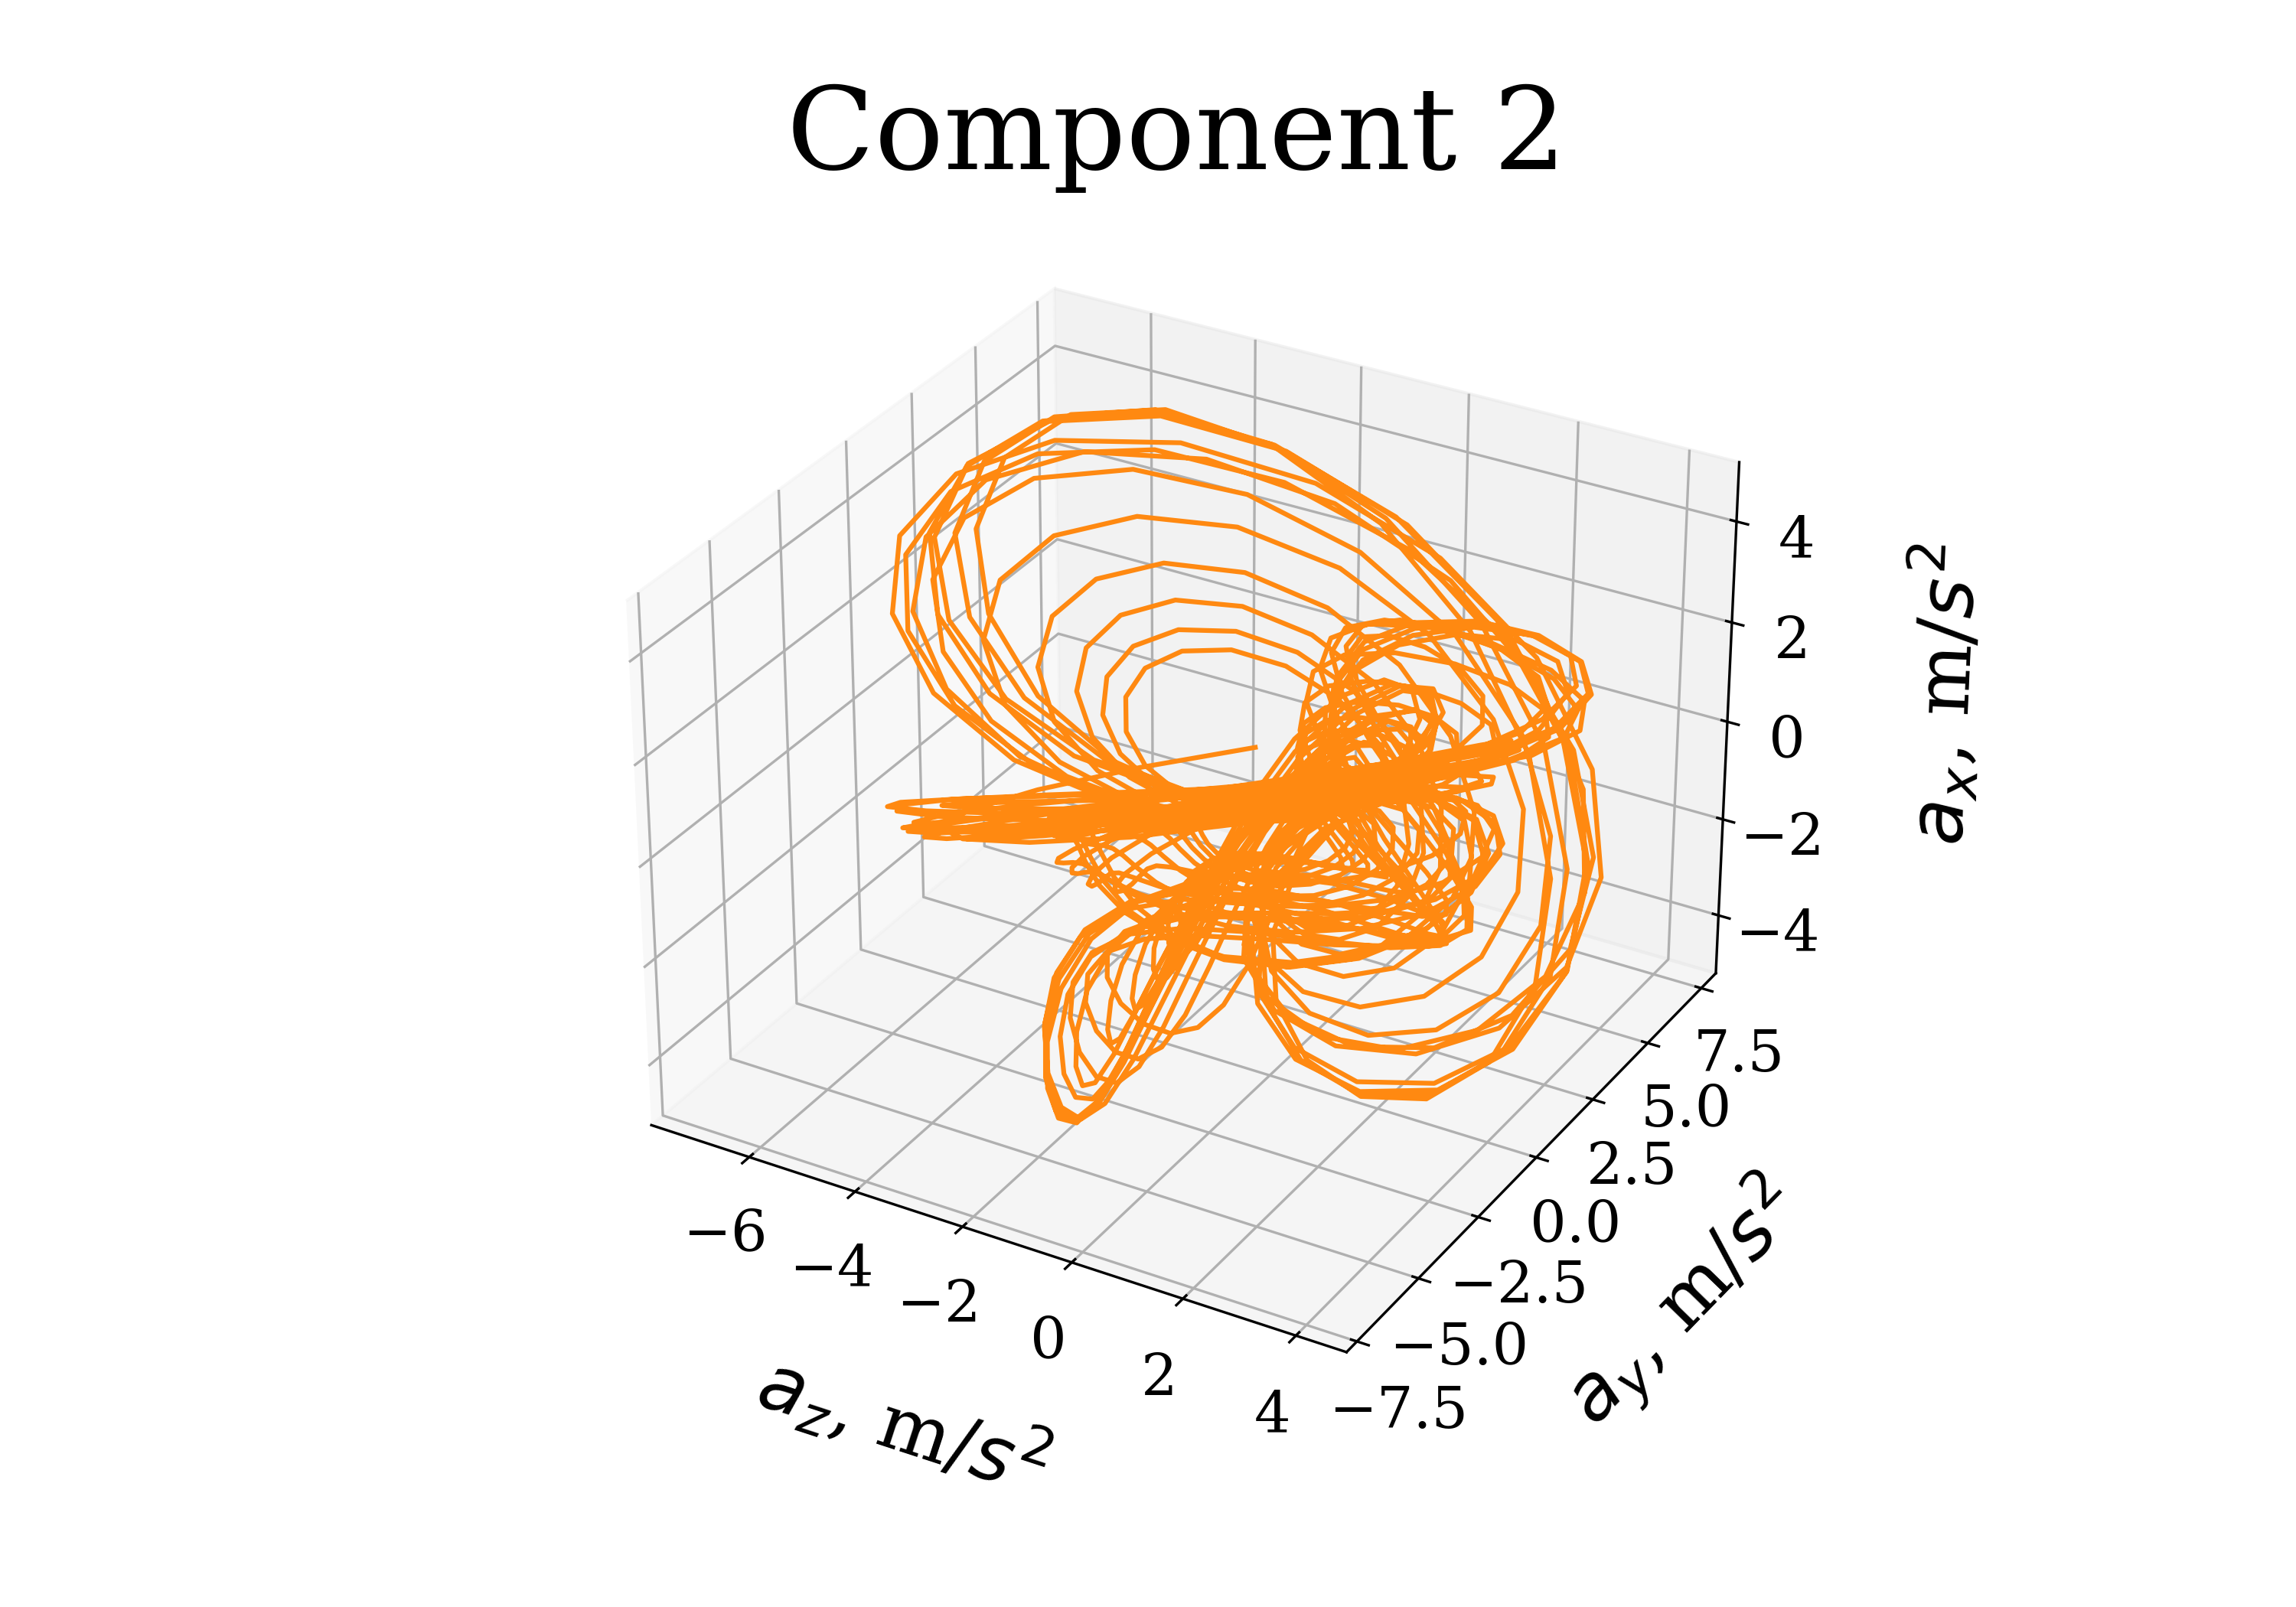
\includegraphics[width=0.48\textwidth, keepaspectratio]{acceler_2.png}
		\caption{tSSA decomposition for the accelerometer data. CPD rank $ = 10 $}\label{fig:accel_decomp_tssa}
	\end{figure}
	
	\begin{figure}[h]
		\centering
		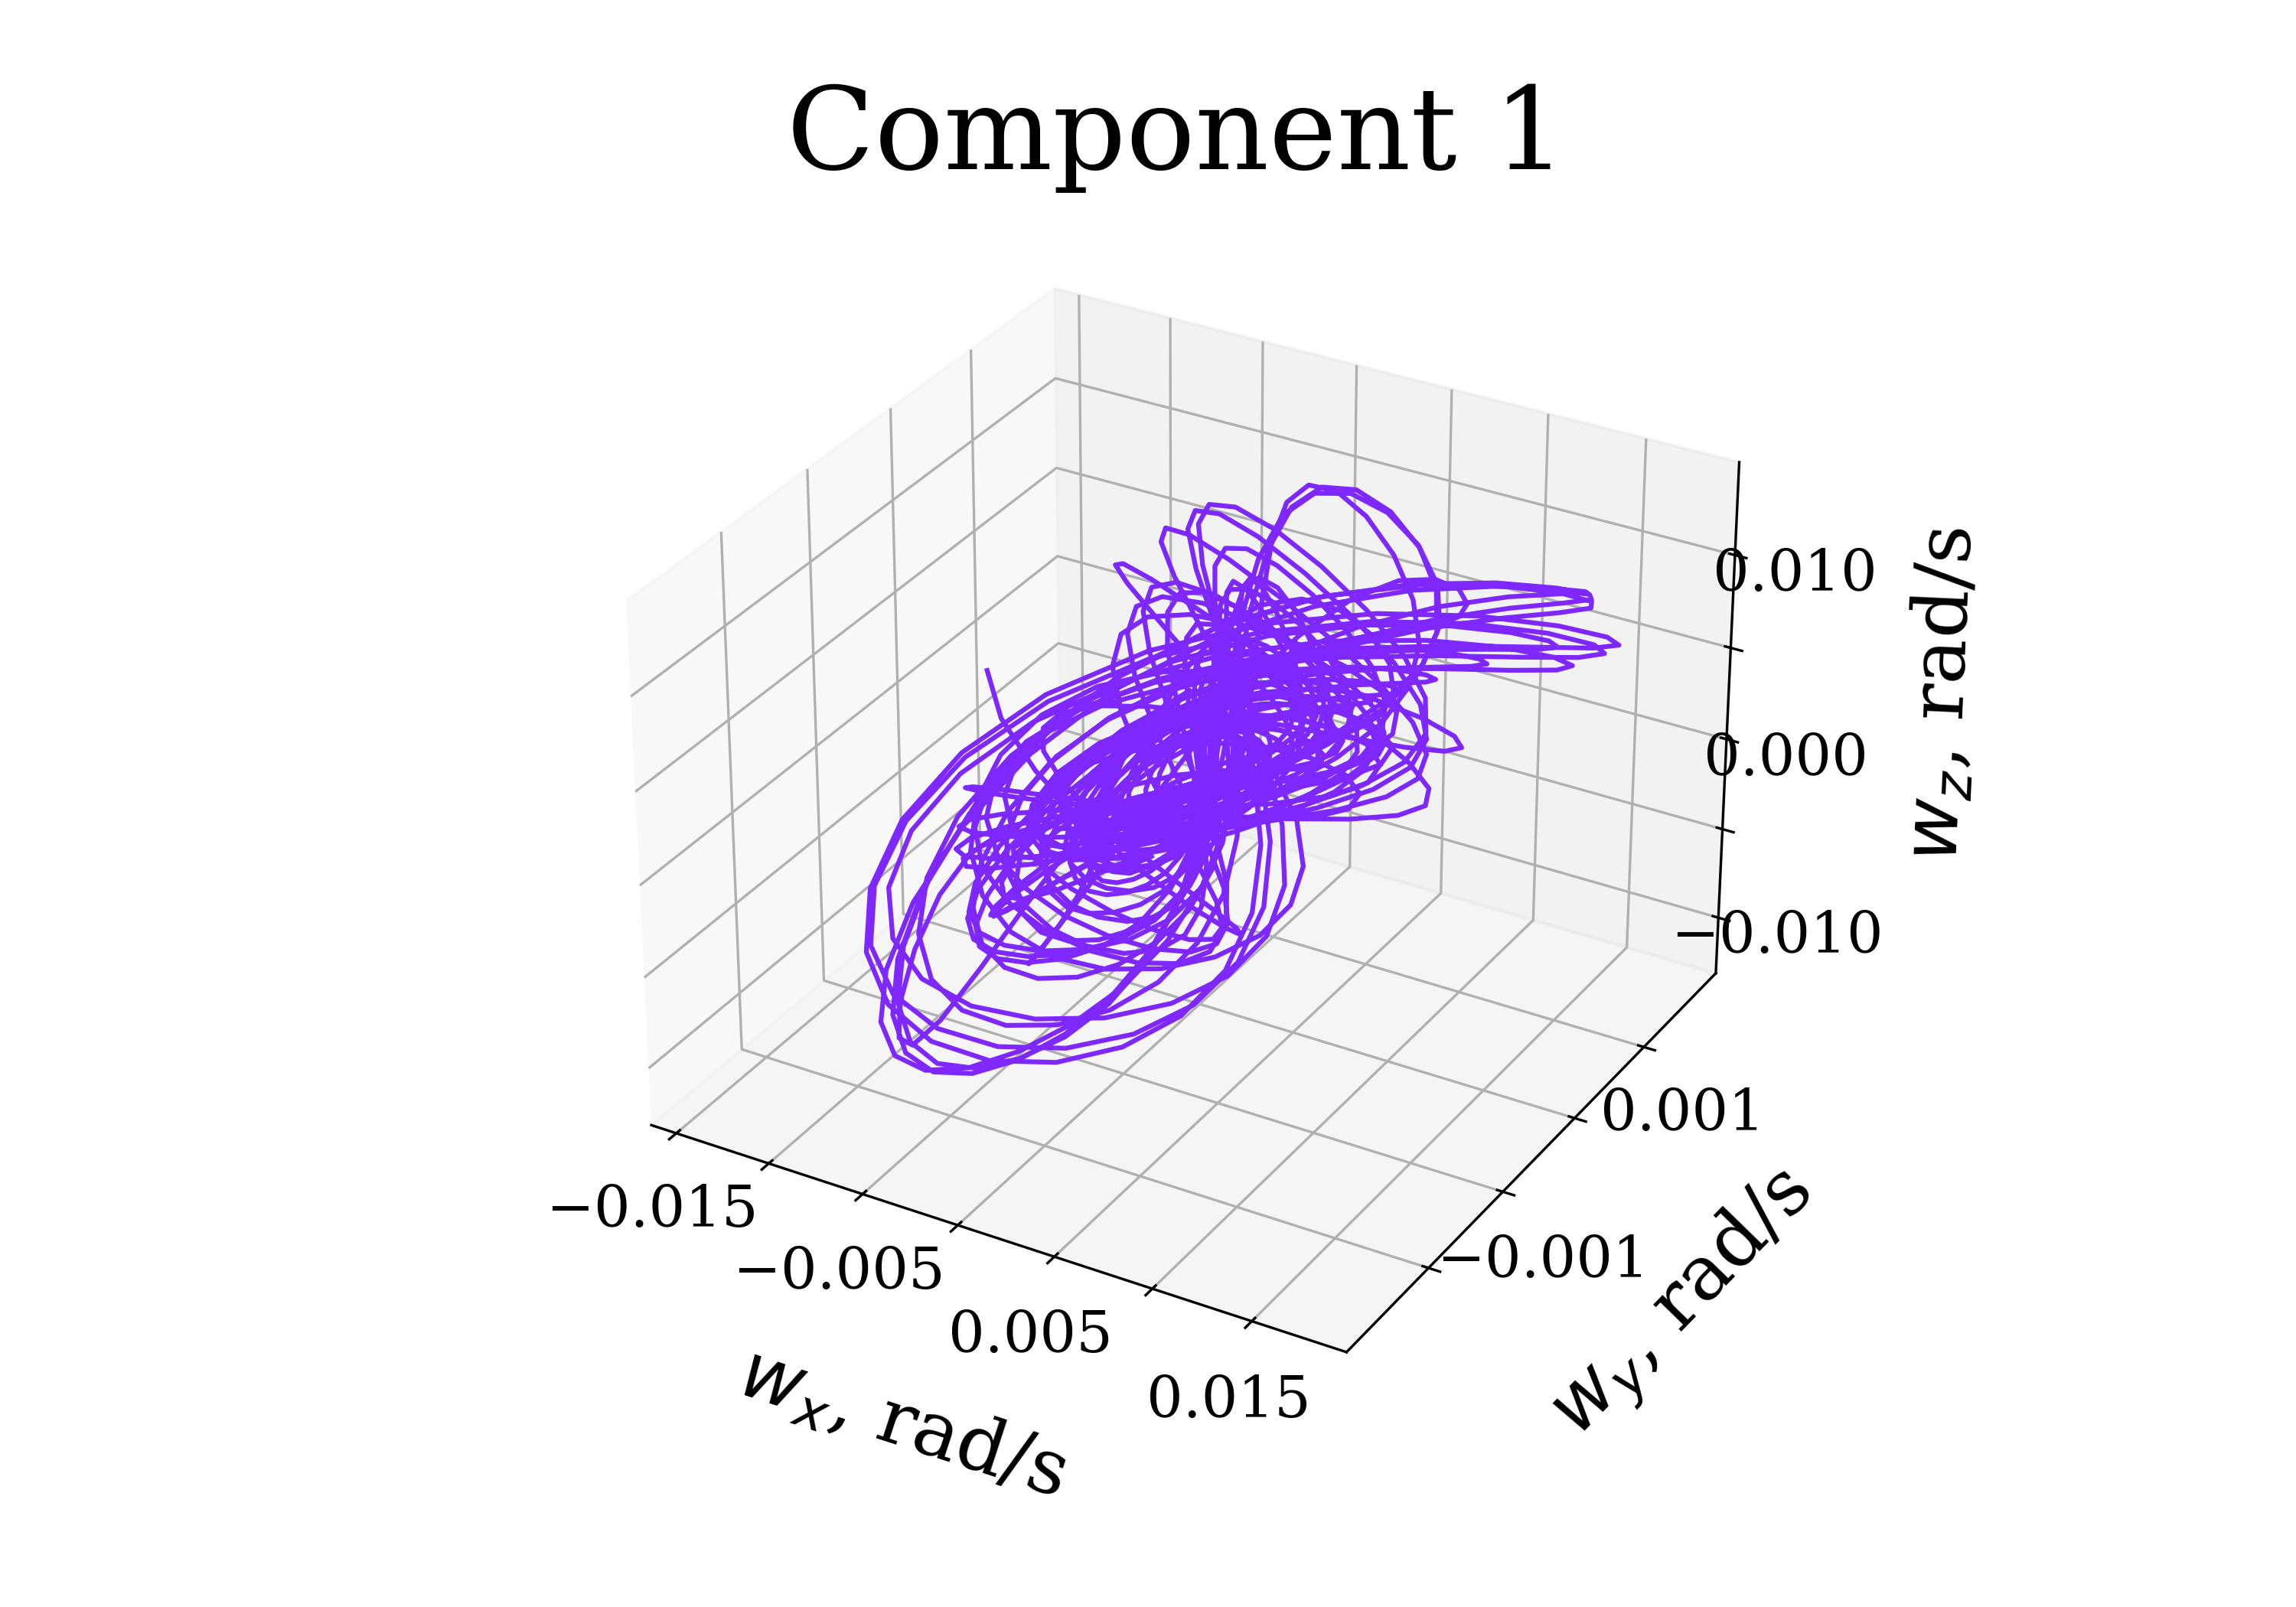
\includegraphics[width=0.48\textwidth, 	keepaspectratio]{gyro_1.png}
		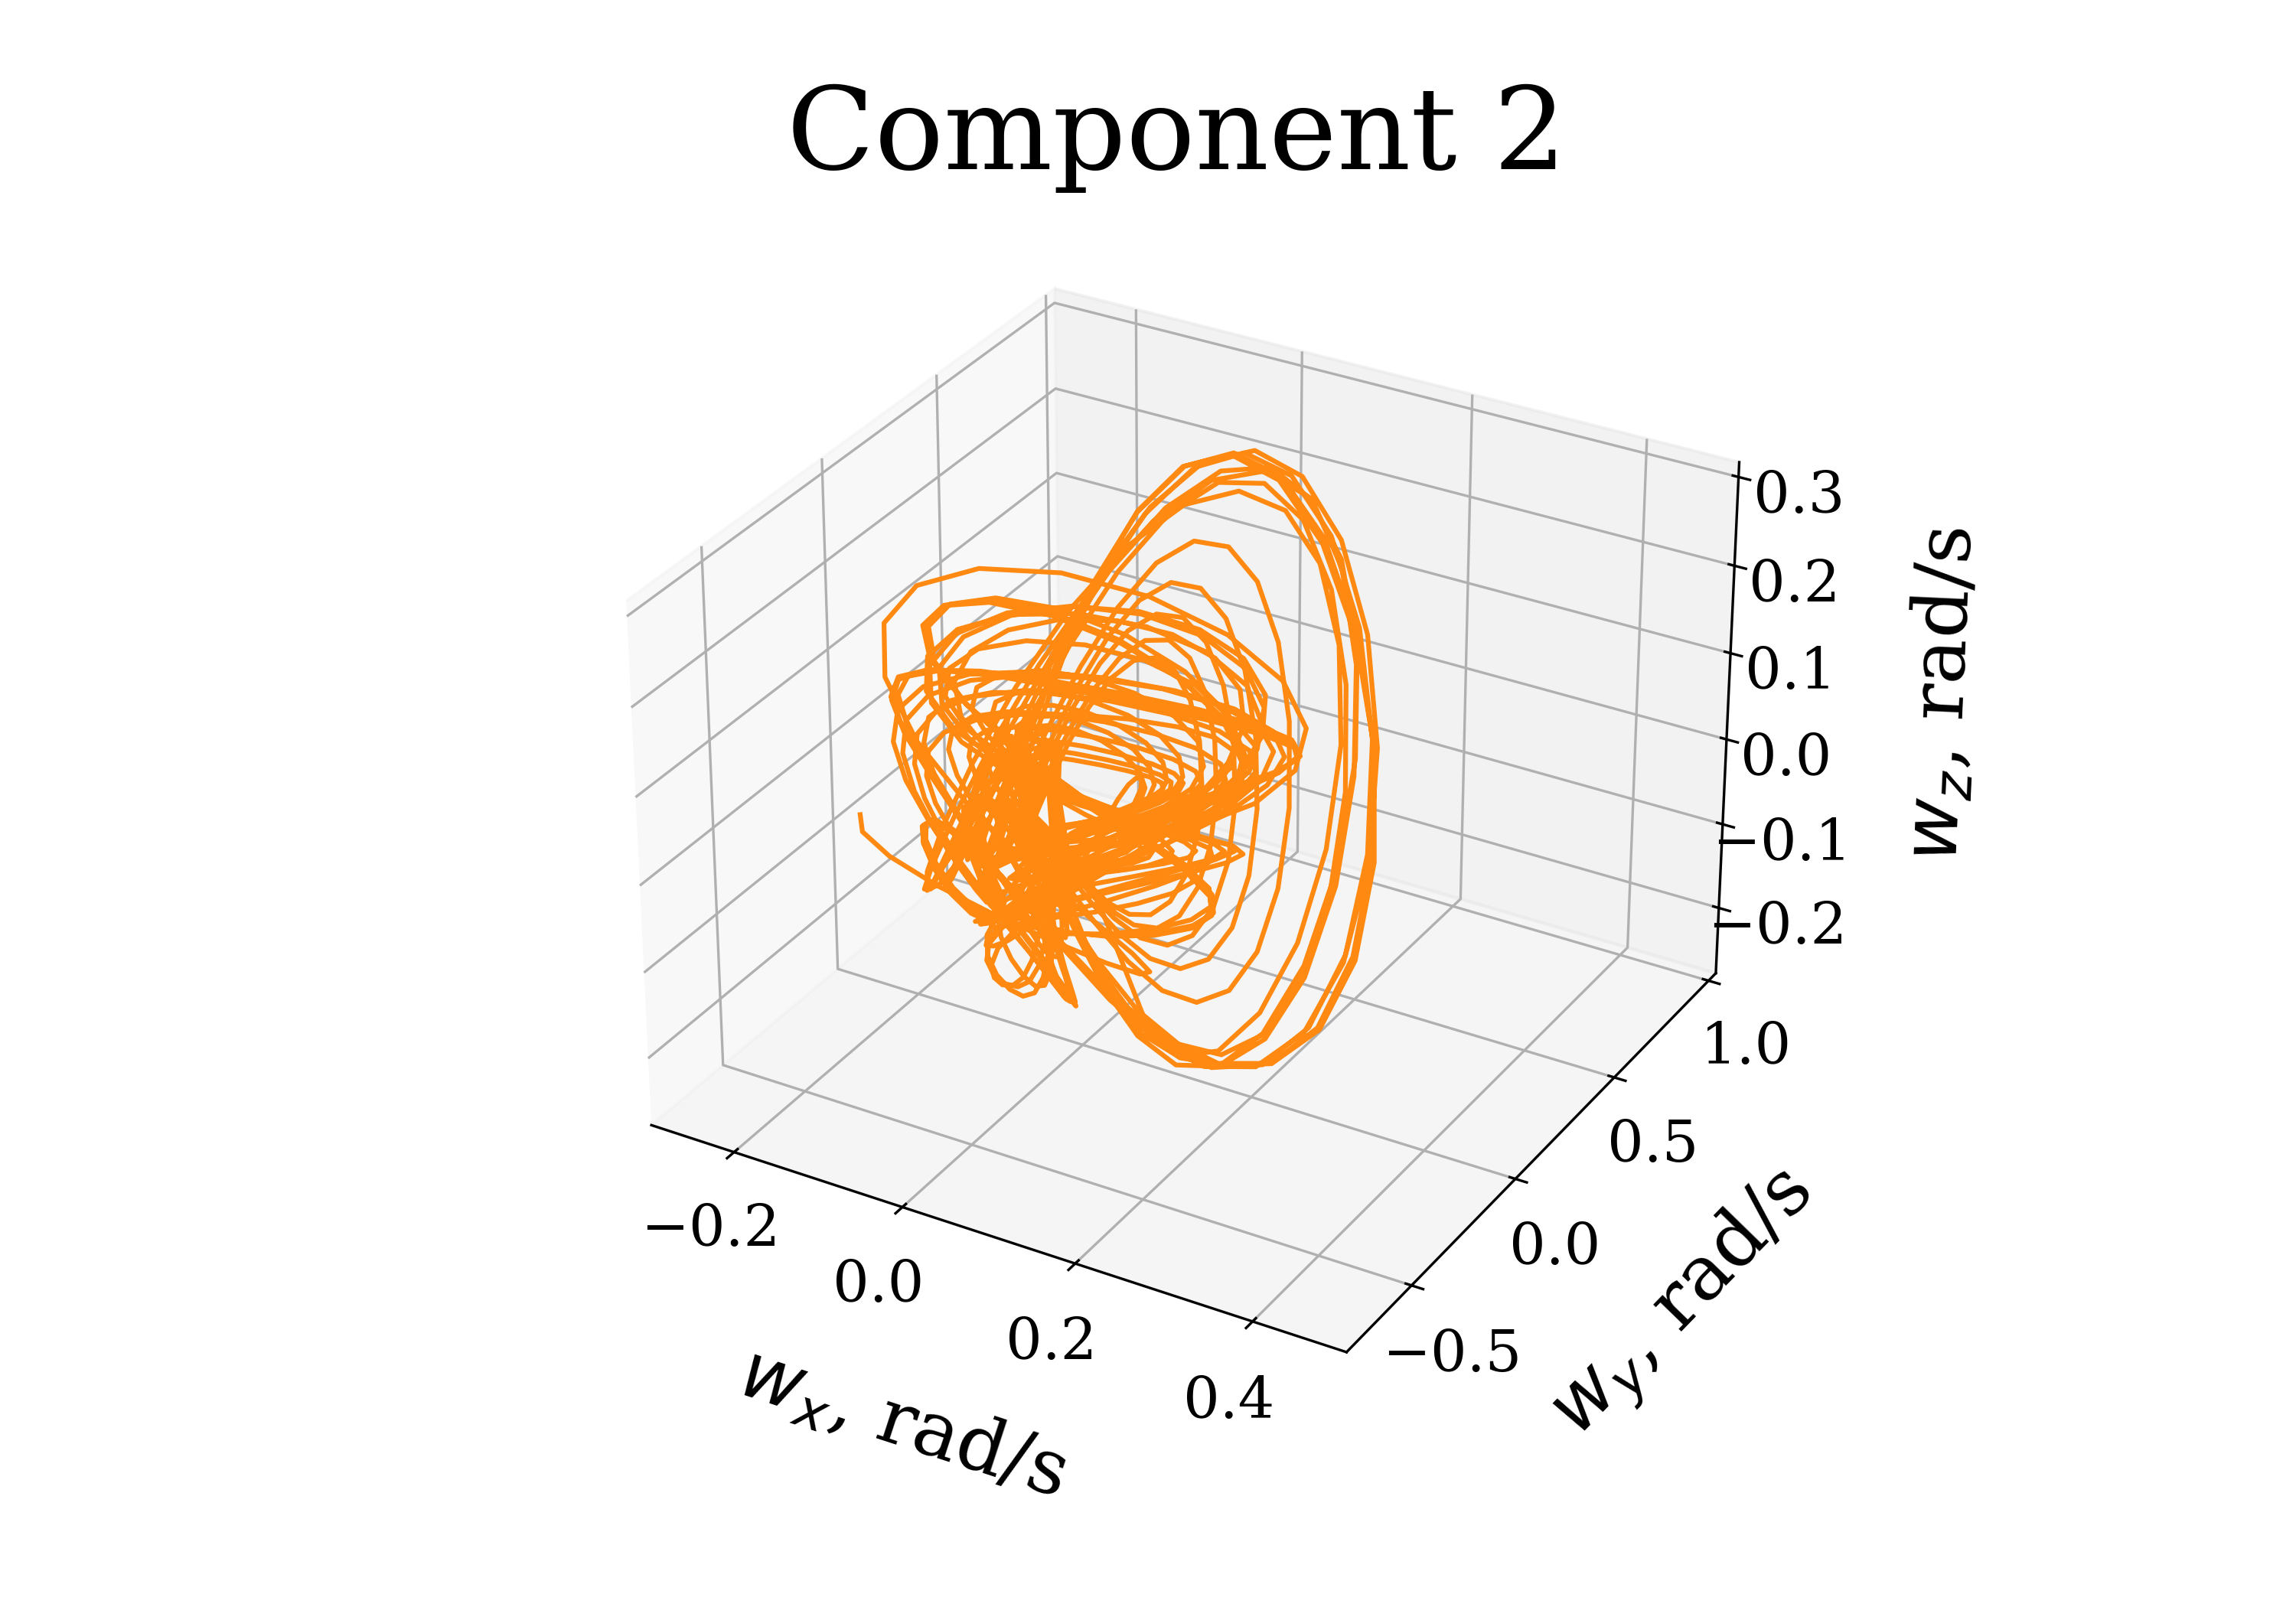
\includegraphics[width=0.48\textwidth, keepaspectratio]{gyro_2.png}
		\caption{tSSA decomposition for the gyroscope data. CPD rank $ = 10 $}\label{fig:gyro_decomp_tssa}
	\end{figure}
	
	Tab. \ref{tab:decomp_electr_results} and \ref{tab:decomp_motion_results} shows the tSSA have lower decomposition quality than the mSSA. It is connected with the two factors. First, the mSSA decomposition is connected with the factors partitioning like the tSSA. Several heuristics exist to obtain usually high-RHE components. On the other hand, the tSSA optimal decomposition problem (\ref{eq:decomp_search_final}) is the Integer Least Squares (ILS) problem, see the end of the Sec.~\ref{sec:optimal_decomp}. It can not be solved efficiently, only approximate methods are available. Moreover, the matrix $ \Lambda $ involved in the ILS has a large row dimension. To shorten computation time, only several hundred rows were left. It is still much greater then the size of the sought parameter vector. But such approximation is not equal to the initial problem.
	
	\def\arraystretch{1.2}
	\begin{table}[h!]
		\centering
		\caption{Decomposition quality of the models for the electricity data}\label{tab:decomp_electr_results}
		\begin{tabular}{|l|c|c|}
			\hline
			\diagbox{Metric}{Method} & tSSA  & mSSA           \\ \hline
			$ \overline{\text{RHE}}_{\text{Producution}} $  & 0.507 & 0.308          \\ \hline
			$ \overline{\text{RHE}}_{\text{Price}} $      & 0.511 & 0.310          \\ \hline
			$ \overline{\text{RHE}} $             & 0.509 & \textbf{0.309} \\ \hline
		\end{tabular}
	\end{table}
	
	\def\arraystretch{1.2}
	\begin{table}[h!]
		\centering
		\caption{Decomposition quality of the models for the inertial unit data}\label{tab:decomp_motion_results}
		\begin{tabular}{|l|c|c|}
			\hline
			\diagbox{Metric}{Method} & tSSA  & mSSA           \\ \hline
			$ \overline{\text{RHE}}_{\text{Accel}} $   & 0.438 & 0.394          \\ \hline
			$ \overline{\text{RHE}}_{\text{Gyro}} $ & 0.732 & 0.468          \\ \hline
			$ \overline{\text{RHE}} $         & 0.585 & \textbf{0.431} \\ \hline
		\end{tabular}
	\end{table}	
	
	\section{Conclusion}
	
		The tSSA method is devoted to the forecast and the additive decomposition of the interdependent multivariate time series. It is based on dynamical systems theory and explicitly build the shared phase space of the series. It also exploits multilinearity of the data via tensor data representation. The method has only two adjustable parameters and require the CPD computation of the trajectory tensor. The tSSA forecast is vector's scalar product. The tSSA decomposition is matrix factorization and factor's partitioning. Finally, the computational experiment showed tSSA's high forecast quality. For the electricity data, the tSSA has the best forecast. The MSE metric is 21\% less then the second best forecast. The MAPE metric is 35\% less than the other methods on average. The tSSA also reduced dimensionality of the electricity data in 16 times.
		
		Future research will be devoted to a new way of building the shared phase space. Then, the current decomposition concept results in a computationally complex problem. Finding new concepts to build additive components is the other direction for the method's improvement.
		
		\bibliography{lit}
	
 \end{document}